\documentclass[aspectratio=169,dvipsnames]{beamer}

%%%% Standard packages
\usepackage[latin1]{inputenc}
\usepackage{graphicx}
\usepackage{amsmath,mathrsfs}
\usepackage{acro}
% Handle hyperlinks
\usepackage{hyperref}
% TikZ & PGF for drawings & flow-charts
\usepackage{pgffor,pgfplots}
\usepackage{tikz}
\usetikzlibrary{arrows, automata}
\usetikzlibrary{spy}
\usetikzlibrary{matrix}
\usetikzlibrary{overlay-beamer-styles}
\usetikzlibrary{positioning}
\usepackage{tikz-cd}
\usetikzlibrary{shapes,arrows}
% Animations
%\usepackage{movie15}
\usepackage{animate}
\usepackage{media9}
% Handling tables
\usepackage{multirow}
\usepackage{pgfplotstable}
\usepackage{booktabs,colortbl}
% Packages for typesetting algorithms and good looking pseudocode 
\usepackage{algorithm}
\usepackage[noend]{algpseudocode}
\renewcommand{\thealgorithm}{}
% Quotations
\usepackage[style=british]{csquotes}
% Handling references
%\usepackage{bibentry}
\usepackage{apacite}
\let\cite\shortcite


%%%% Settings 
%% Settings for hyperref
\hypersetup{%
    bookmarks=true,         % show bookmarks bar?
    pdfmenubar=true,       % show Acrobat's menu?
    pdffitwindow=false,     % window fit to page when opened
    pdfstartview={FitH},    % fits the width of the page to the window
    colorlinks=true,       % false: boxed links; true: colored links
    linkcolor=red,          % color of internal links
    citecolor=gray,        % color of links to bibliography
    filecolor=blue,      % color of file links
    urlcolor=blue,           % color of external links
    pdfborder = {0,0,0}
}
%% Settings for the beamer class.
% Select presentation mode  
\mode<presentation>{%
  \usetheme[height=14mm]{Rochester}
  \setbeamertemplate{items}[ball] 
  \setbeamertemplate{blocks}[rounded][shadow=true]   
  \setbeamertemplate{navigation symbols}{}   
  \setbeamercovered{transparent}
  \setbeamertemplate{footline}{\hfill \insertframenumber/\inserttotalframenumber \quad}
}
%  Remove navigation buttons
\beamertemplatenavigationsymbolsempty 
% Place logos in the title page
\titlegraphic{%
  \vskip-3\baselineskip
  
\includegraphics[height=35pt]{SSF_Logotype}
  \hfill
  
\includegraphics[height=35pt]{KTH_Logotype}
}
% Declare image layers
\pgfdeclarelayer{background layer} 
\pgfdeclarelayer{foreground layer}
\pgfsetlayers{background layer,main,foreground layer}
% For every picture that defines or uses external nodes, you'll have to
% apply the 'remember picture' style. To avoid some typing, we'll apply
% the style to all pictures.
\tikzstyle{every picture}+=[remember picture]
% By default all math in TikZ nodes are set in inline mode. Change this to
% displaystyle so that we don't get small fractions.
\everymath{\displaystyle}
%% Table 
\setlength{\heavyrulewidth}{0.1em}
\newcommand{\otoprule}{\midrule[\heavyrulewidth]}
%% Location of images, requires 'graphicx' package
\graphicspath{%
  {images/}
  {images/General/}
  {images/LogoTypes/}
  {images/NN_Advesarial/}
  {images/NN_Architectures/}
  {images/NN_Basics/}
  {images/NN_Basics/NNanimation/}
  {images/NN_Optimization/}
  {images/NN_Optimization/animations/}
  {images/NN_Optimization/animations/BealeFunction/}
  {images/NN_Optimization/animations/LongValley/}
  {images/NN_Optimization/animations/SaddlePoint/}
  {images/NN_Examples/}
  {images/NN_Examples/RNN/}
  {images/NN_Examples/ColorRestoration/}
  {images/NN_Examples/ImageClassification/}
  {images/NN_Examples/ImageCaptioning/}
  {images/NN_Examples/SpeechRecognition/}
  {images/NN_Examples/MachineTranslation/}
  {images/NN_Examples/SelfDrivingCar/} 
  {images/NN_Examples/Games/} 
  {images/NN_Examples/PixelRestoration/} 
  {images/NN_Examples/StyleTransfer/} 
  {images/NN_Trouble/} 
}
%% TikZ
\tikzset{basic/.style={draw,fill=blue!20,text width=1em,text badly centered}}
\tikzset{input/.style={basic,circle}}
\tikzset{weights/.style={basic,rectangle}}
\tikzset{functions/.style={basic,circle,fill=blue!10}}

%%%% Acronyms
\DeclareAcronym{CNN}{
  short = CNN,
  long = convolutional neural network}
\DeclareAcronym{RNN}{
  short = RNN,
  long = recurrent neural network}
\DeclareAcronym{VC}{
  short = VC,
  long = Vapnik-Chervonenkis}
\DeclareAcronym{ReLU}{
  short = ReLU,
  long = rectified linear unit}
\DeclareAcronym{SGD}{
  short = SGD,
  long = stochastic gradient decent}
\DeclareAcronym{CM}{
  short = CM,
  long = conditional mean}
\DeclareAcronym{MAP}{
  short = MAP,
  long = maximum a posteriori}
\DeclareAcronym{DAG}{
  short = DAG,
  long = directed acyclic graph}
\DeclareAcronym{NAG}{
  short = NAG,
  long = Nesterov accelerated gradient}
\DeclareAcronym{EMA}{
  short = EMA,
  long = exponential moving average}
\DeclareAcronym{RMS}{
  short = RMS,
  long =  root mean squared}
\DeclareAcronym{AdaGrad}{
  short = AdaGrad,
  long =  adaptive gradient algorithm}
\DeclareAcronym{AdaDelta}{
  short = AdaDelta,
  long =  AdaDelta}
\DeclareAcronym{RMSProp}{
  short = RMSProp,
  long =  root mean square propagation}
\DeclareAcronym{ADAM}{
  short = Adam,
  long =  adaptive moment estimation}
  
%%%% Macros
% Sets, spaces, etc
\newcommand{\Real}{\mathbb{R}}
\newcommand{\Natural}{\mathbb{N}}
\newcommand{\Class}[1]{\mathscr{#1}}
\newcommand{\ModelClass}{\Class{M}}
\newcommand{\LClass}{\Class{L}}
\newcommand{\InputSpace}{X}
\newcommand{\OutputSpace}{Y}
\newcommand{\HSpace}{H}
\newcommand{\HSpaceOther}{H'}
\newcommand{\RecSpace}{X}
\newcommand{\DataSpace}{Y}
\newcommand{\ParamSet}{\triangle}
\newcommand{\VecSpace}{X}
\newcommand{\VecSpaceSAlg}{\SAlg{\VecSpace}}
% Operators
\newcommand{\Op}[1]{\operatorname{\mathcal{#1}}}
\newcommand{\ForwardOp}{\Op{A}}
\newcommand{\ForwardOpPseduoInv}{\ForwardOp^{\dagger}}
\newcommand{\LinMap}{\Op{W}}
\newcommand{\NonLinMap}{\Psi}
\newcommand{\Activation}{\psi}
\DeclareMathOperator*{\argmin}{arg\,min}
\DeclareMathOperator{\dist}{d}
\DeclareMathOperator{\Dropout}{Dropout}
\DeclareMathOperator{\Pool}{Pool}
\DeclareMathOperator{\Rad}{Rad}
\DeclareMathOperator{\rank}{rank}
\DeclareMathOperator{\EMA}{EMA}
\DeclareMathOperator{\RMS}{RMS}
\DeclareMathOperator{\diag}{diag}
\DeclareMathOperator{\Id}{Id}
% Elements
\newcommand{\velem}{x}
\newcommand{\velemother}{y}
\newcommand{\inputvar}{x}
\newcommand{\outputvar}{y}
\newcommand{\signal}{x}
\newcommand{\signaltrue}{\signal^*}
\newcommand{\data}{y}
\newcommand{\param}{\theta}
\newcommand{\paramupdt}{\triangle \param}
% Probabilistic notions
\newcommand{\ProbMeas}{\mathbb{P}}
\newcommand{\StatModel}{\mathscr{S}}
\newcommand{\Prob}{\mathbb{P}}
\newcommand{\PClass}[1]{\mathscr{P}_{#1}}
\newcommand{\SAlg}[1]{\mathfrak{S}_{#1}}
\newcommand{\RecSpaceSAlg}{\SAlg{\RecSpace}}
\newcommand{\DataSpaceSAlg}{\SAlg{\DataSpace}}
\newcommand{\DecisionSpace}{\ensuremath{D}}
\newcommand{\DecisionSpaceSAlg}{\SAlg{\DecisionSpace}}
\DeclareMathOperator{\Expect}{\mathbb{E}}
\DeclareMathOperator{\Risk}{\mathcal{R}}
\newcommand{\stochastic}[1]{\mathsf{#1}}
\newcommand{\DataModel}{\mathcal{M}}
\newcommand{\stvelem}{\stochastic{\velem}}
\newcommand{\stvelemother}{\stochastic{\velemother}}
\newcommand{\stsignal}{\stochastic{\signal}}
\newcommand{\stdata}{\stochastic{\data}}
\newcommand{\stparam}{\stochastic{\param}}
\newcommand{\stinputvar}{\stochastic{\inputvar}}
\newcommand{\stoutputvar}{\stochastic{\outputvar}}
\newcommand{\stsigma}{\stochastic{\sigma}}
\newcommand{\ProbSignalTrue}{\mu^*}
\newcommand{\prior}{\pi_{\text{prior}}}
\newcommand{\likelihood}[2]{\pi_{\text{liklh}}\left(#1 \left\mid\right. #2\right)}
\newcommand{\posterior}[2]{\pi_{\text{post}}\left(#1 \left\mid\right. #2\right)}
\DeclareMathOperator{\drule}{\mathcal{D}}
% NN notions
\newcommand{\Learn}{\mathcal{L}}
\newcommand{\NNMatrix}{\boldsymbol{W}}
\newcommand{\tData}{\Sigma}
\newcommand{\vData}{\Sigma_0}
\newcommand{\objective}{\Op{J}}
\newcommand{\objGrad}{\nabla_{\!\param}\! \objective}
\newcommand{\model}{\Op{A}}
\newcommand{\optimParam}{\param^*}
\newcommand{\optimParamEmp}{\widehat{\param}^*}
\DeclareMathOperator{\pregfunc}{\mathcal{S}}
\DeclareMathOperator{\loss}{\ell}
\DeclareMathOperator{\Rademacher}{Rad}
\newcommand{\depth}{d}
\newcommand{\layerdim}{n}
\newcommand{\paramdim}{N}
\newcommand{\trainData}{\Sigma_{\text{train}}}
\newcommand{\trainDatadim}{m}
\newcommand{\trainProbMeas}{\tmu_{\text{train}}}
\newcommand{\trainError}{\epsilon_{\text{train}}}
\newcommand{\testData}{\Sigma_{\text{test}}}
\newcommand{\testDatadim}{{m'}}
\newcommand{\testProbMeas}{\tmu_{\text{test}}}
\newcommand{\testError}{\epsilon_{\text{test}}}
\newcommand{\genError}{\epsilon_{\text{gen}}}
\newcommand{\tmu}{\widehat{\mu}}
% Other
\newcommand{\advantage}{\textcolor{PineGreen}{$\boldsymbol{+}$}}
\newcommand{\drawback}{\textcolor{WildStrawberry}{$\boldsymbol{-}$}}
\newcommand{\slideTitle}[1]{\begin{center}{\Huge \structure{#1}}\end{center}}

% Preamble 
\title{Lecture 1: Introduction to machine learning and some of its underlying mathematics}
\author{Ozan �ktem \and Jonas Adler}
\institute{Department of Mathematics \\ KTH - Royal Institute of Technology, Stockholm}
\date{April 11, 2018 \\ 
Mini-course: Mathematics of Deep Learning \\ with an Emphasis on Inverse Problems \\[0.5em]
Georg-August-Universit�t G�ttingen}

\begin{document}
\maketitle

% Frame
\begin{frame}[plain]
\blockquote[Albert Einstein][]{If we knew what it was we were doing, it would not be called research, would it?}
\end{frame}

% Frame
\begin{frame}[plain]
\centering
\begin{tikzpicture}[remember picture,overlay]
  \node[anchor=south west, inner sep=0pt,xshift=0.075\textwidth,yshift=0.1\textheight] at (current page.south west) 
  {%
    \includemedia[%
     % draft,
     addresource=./movies/dynamicsClassify.mp4,
     activate=pageopen,transparent,
     flashvars={source=./movies/dynamicsClassify.mp4},
     width=\textwidth,
     height=\textheight
   ]{}{VPlayer.swf}
  };
\end{tikzpicture}
\end{frame}

% Frame
\begin{frame}[plain]
\centering
\begin{tikzpicture}[remember picture,overlay]
  \node[anchor=south west, inner sep=0pt,xshift=0.075\textwidth,yshift=0.1\textheight] at (current page.south west) 
  {%
    \includemedia[%
      % draft,
      addresource=./movies/PeaksStable.mp4,
      activate=pageopen,transparent,
      flashvars={source=./movies/PeaksStable.mp4},
      width=\textwidth,
      height=\textheight
    ]{}{VPlayer.swf}
  };
\end{tikzpicture}
\end{frame}

% Frame
\begin{frame}{Lecture overview}
\begin{itemize}
\item Basics of machine learning
\item Type of task: Supervised, unsupervised, and reinforcement learning
\item Network architectures
  \begin{itemize}
  \item Type of networks
  \item Geometric stability
  \item Activation functions
  \item Model capacity and complexity
  \end{itemize}
\item Supervised learning 
  \begin{itemize}
  \item Types of errors: Generalisation gap
  \item Optimisation methods
  \item Stability
  \item Non-convexity
  \end{itemize}
% \item Generative models   
\end{itemize}
\end{frame}

% Frame
\begin{frame}[plain]
\slideTitle{Basics of machine learning}
\begin{itemize}
\item Terminology
\item History
\item Example applications
\end{itemize}
\end{frame}

% Frame
\begin{frame}{Terminology}
\begin{columns}
\begin{column}{0.6\textwidth}
  \begin{itemize}
  \item \structure{Artificial Intelligence (AI):} Set of general purpose algorithms and technologies that enable 
  machines to effectively perform highly complex tasks that would require `intelligence' if humans were to perform them.
%  such as learning and adaptation; sensory understanding and interaction; 
%  reasoning and planning; optimisation of procedures and parameters; autonomy; creativity; and extracting knowledge and 
%  predictions from large, diverse digital data.
  \item \structure{Machine learning (ML):} Subset of AI that uses statistical decision theory to enable machines to learn from data without being explicitly programmed for a specific task.
  \item \structure{Deep Learning (DL):} A subset of ML where complicated tasks are performed by breaking them down into several layers
\end{itemize}
\end{column}
\begin{column}{0.4\textwidth}
  \centering
  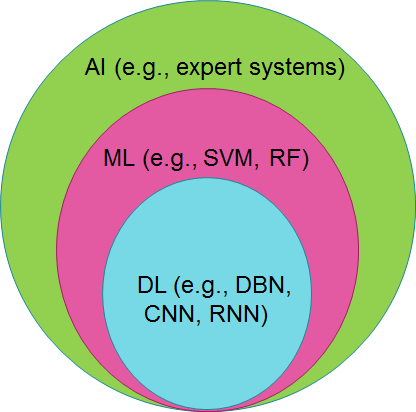
\includegraphics[width=\textwidth]{venn_diagram}
\end{column}
\end{columns}
\end{frame}

% Frame
\begin{frame}{History}

\begin{overprint}
\onslide<1>
\begin{itemize}
\item \structure{Early history (1950--1990)} 
\begin{itemize}
\item First artificial neural network computational machines in 1954
\item The perceptron for pattern recognition introduced in 1958. 
\item First functional networks with many layers introduced in 1965. 
\end{itemize}
\par
\structure{Stagnation:} Basic perceptrons cannot process the exclusive-or circuit (XOR) (1969) and computers not powerful enough.

\item \structure{Backpropagation (1974):} 
Equivalent to chain rule and automatic differentiation in reverse accumulation mode \cite{Werbos:1974aa}.

\item \structure{\Acl{CNN}:} 
\begin{itemize} 
\item \structure{1998:} Handwriting recognition \cite{Lecun:1998aa}. 
\item \structure{2012:} AlexNet \cite{Krizhevsky:2012aa}, a deep \acl{CNN}, wins the 2012 ILSVRC image classification challenge, astounding improvement over the next best entry that shocks the computer vision community. 
\end{itemize}
\end{itemize}
\onslide<2>
\centering
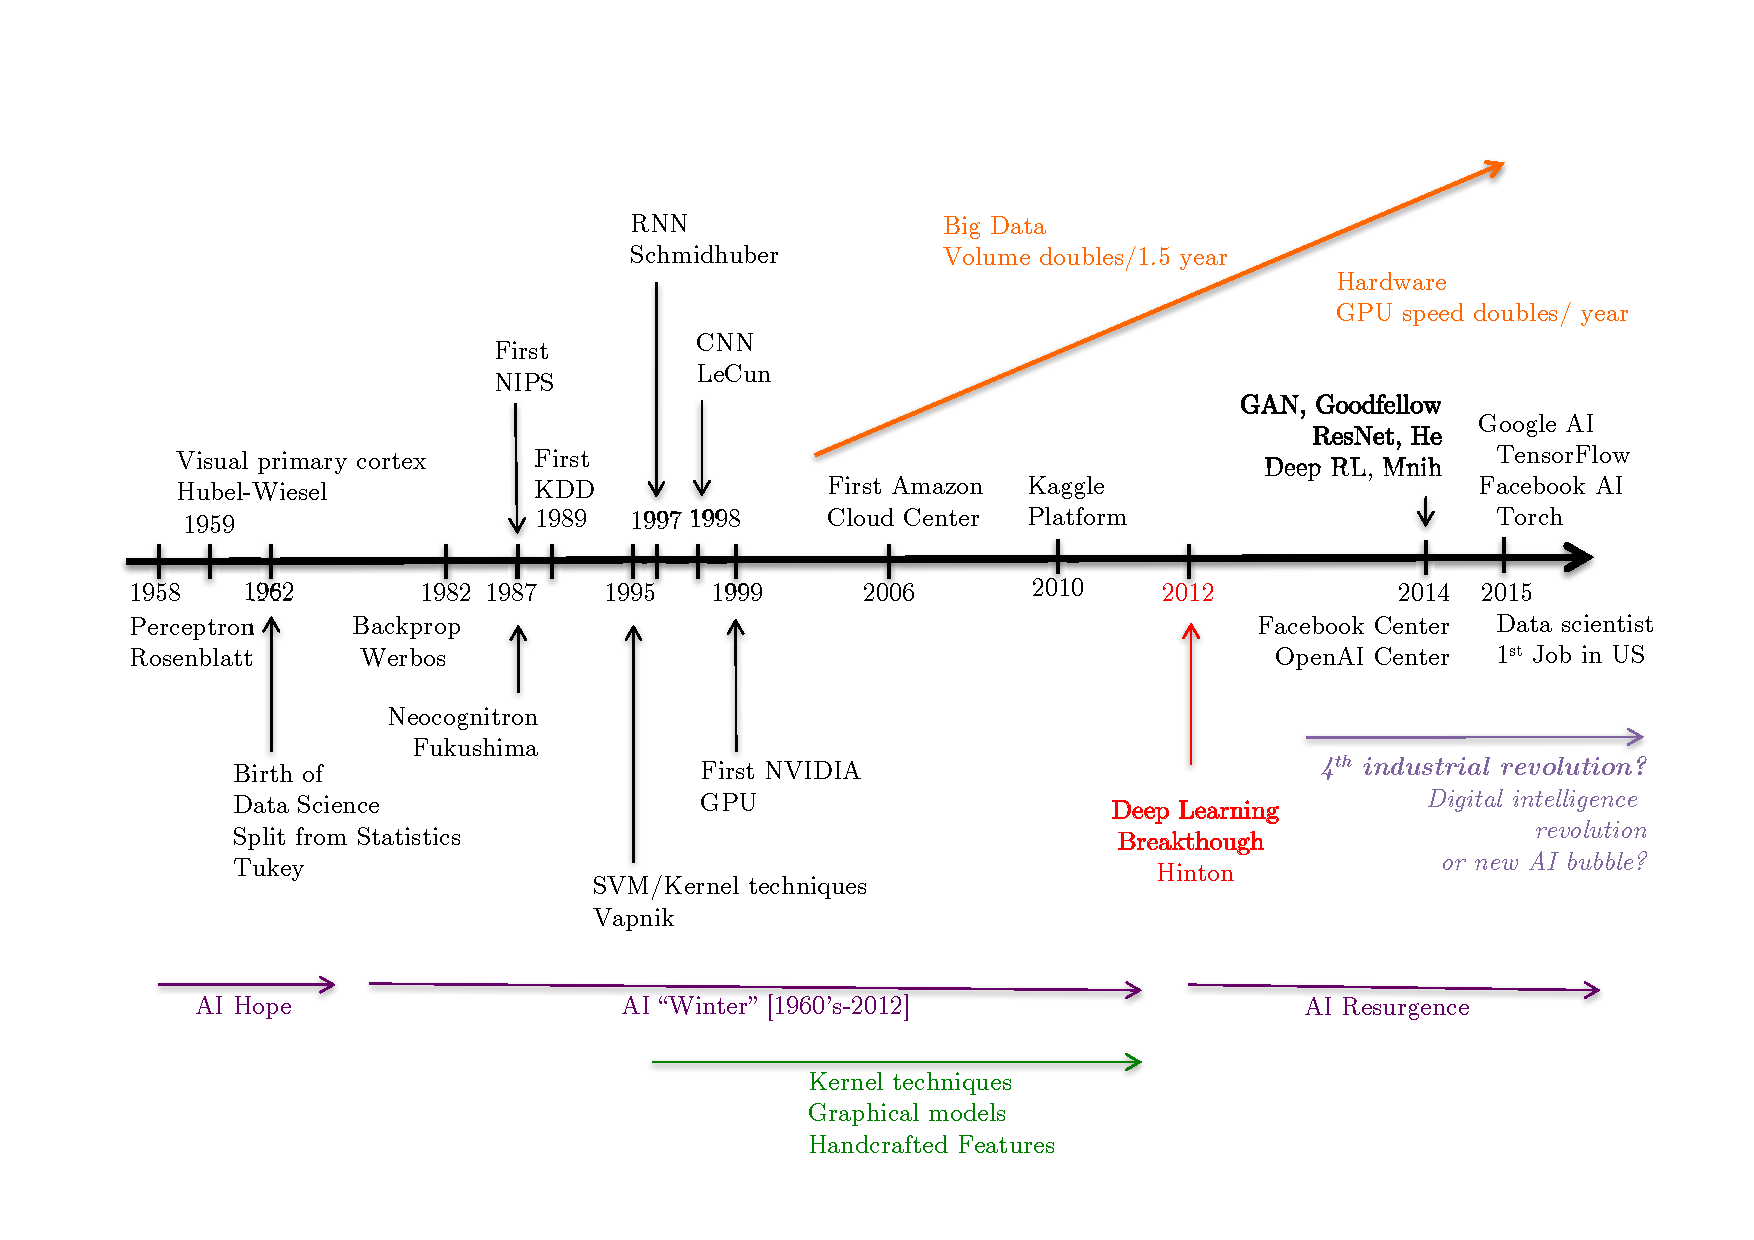
\includegraphics[width=\textwidth]{NN_history}
\end{overprint}
\end{frame}


% Frame
\begin{frame}{Success stories}
% http://www.yaronhadad.com/deep-learning-most-amazing-applications/
\begin{overprint}
\onslide<1>
  \structure{Image classification:} Classify (predict label) for given image
  \begin{columns}[T]
  \begin{column}{0.45\textwidth}
    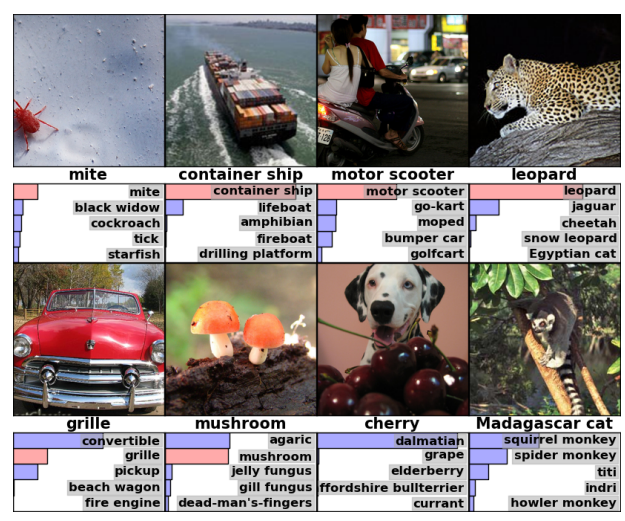
\includegraphics[height=0.7\textheight]{KSH-results}
    \par
    Image, true label \& probabilities for top 5 labels \cite{Krizhevsky:2012aa}.
    % LSVRC-2010 ImageNet has 1.3 million high-resolution images and 1000 different labels.
    % NN has 60 million parameters
    \end{column}
  \begin{column}{0.55\textwidth}
    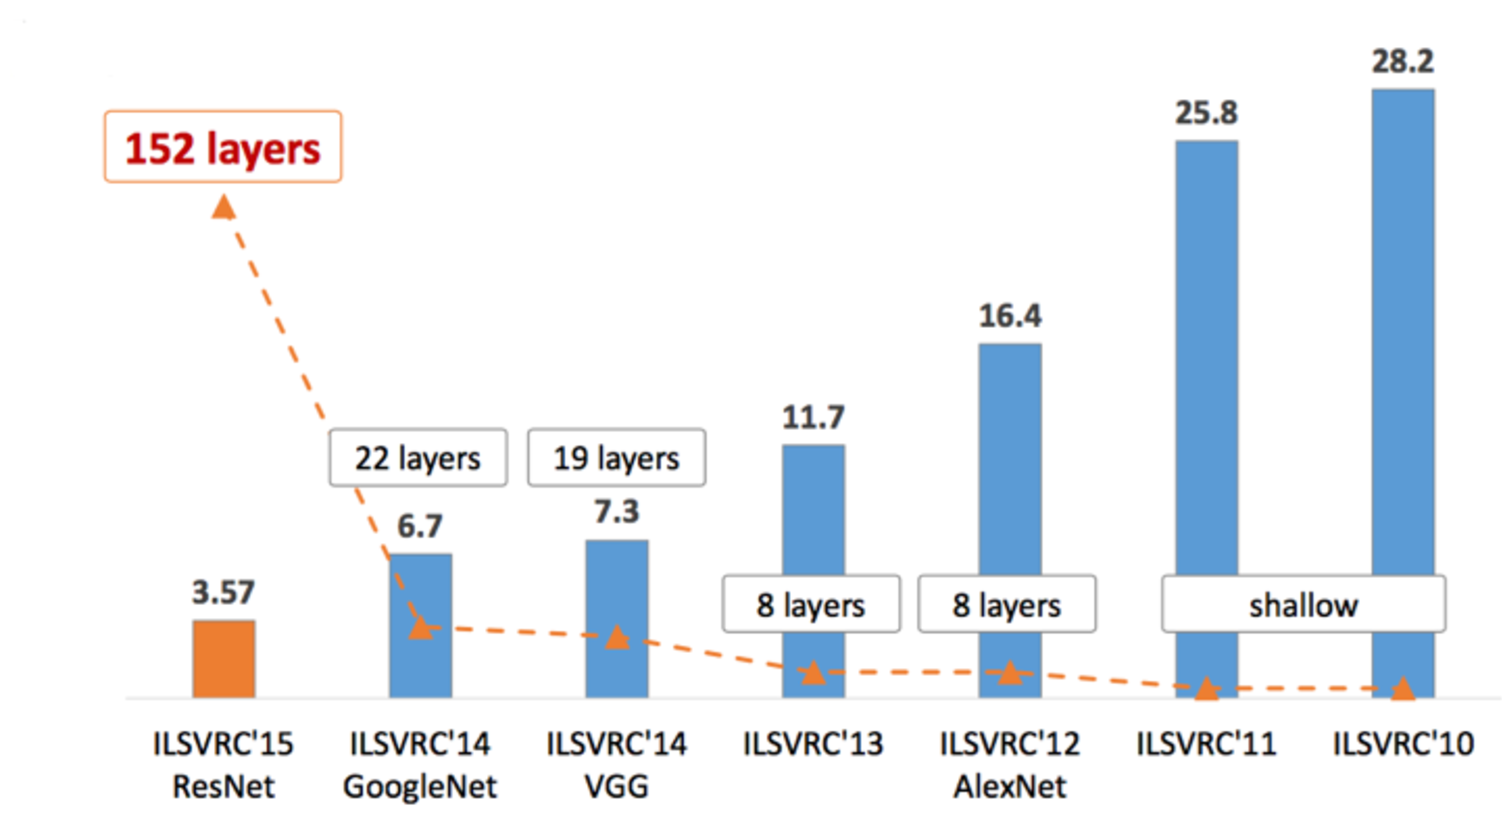
\includegraphics[width=\textwidth]{ImageNet_classification_error_vs_depth}
    \par 
    State-of-the-art deep neural network classifiers \cite{He:2016aa} surpass human capacity ($\sim 5\%$ error).
    % 224�224 images, 1000 labels. The models are trained on the 1.28 million training images, and evaluated on the 50k validation images. Tested on 100k test images
  \end{column}
  \end{columns}
  % LabelMe: consists of hundreds of thousands of fully-segmented images
  % B.C. Russell, A. Torralba, K.P. Murphy, and W.T. Freeman. Labelme: a database and web-based tool for image annotation. International journal of computer vision, 77(1):157?173, 2008.
  % ImageNet: consists of over 15 million labeled high-resolution images in over 22,000 categories.
  % J. Deng, W. Dong, R. Socher, L.-J. Li, K. Li, and L. Fei-Fei. ImageNet: A Large-Scale Hierarchical Image Database. In CVPR09, 2009.
\onslide<2>
  \structure{Pixel restoration (superresolution):} Restore image from low-resolution representation \cite{Dahl:2017aa}.
  \begin{center}
        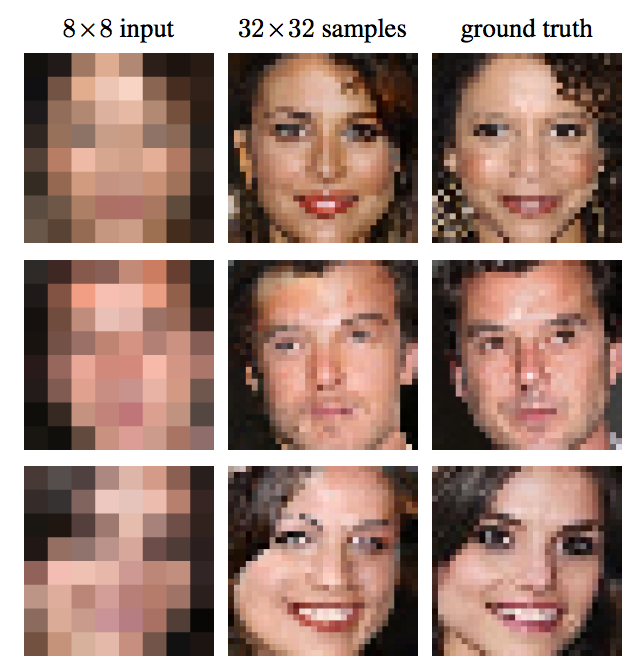
\includegraphics[height=0.75\textheight]{PixelRestoration}
  \end{center}
\onslide<3>
  \structure{Color restoration:} Restore/insert colours in B\&W photos and videos \cite{Iizuka:2016aa}.
  \begin{center}
        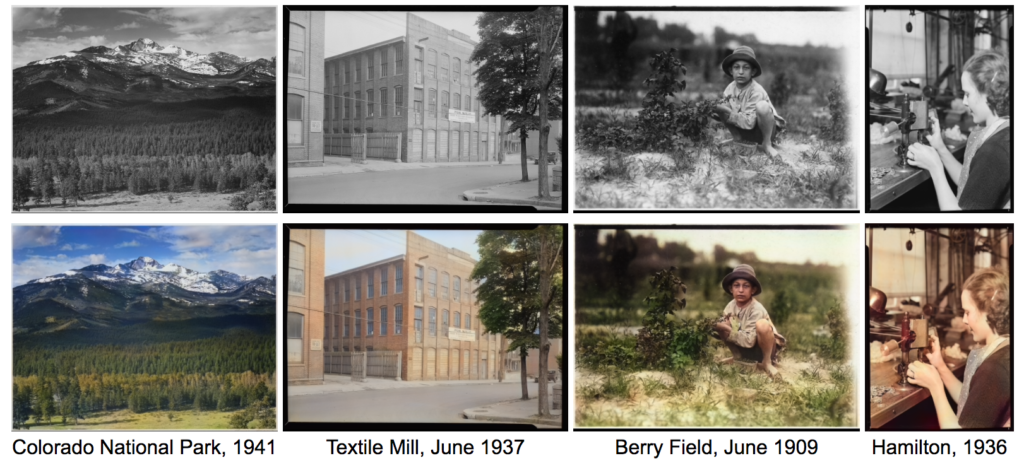
\includegraphics[height=0.75\textheight]{Color_restoration}
  \end{center}
\onslide<4-5>
  \structure{Image captioning:} Generate sentences with proper English grammar that describes contents of image \cite{Karpathy:2017aa}.
  \par\medskip
  \alt<4>{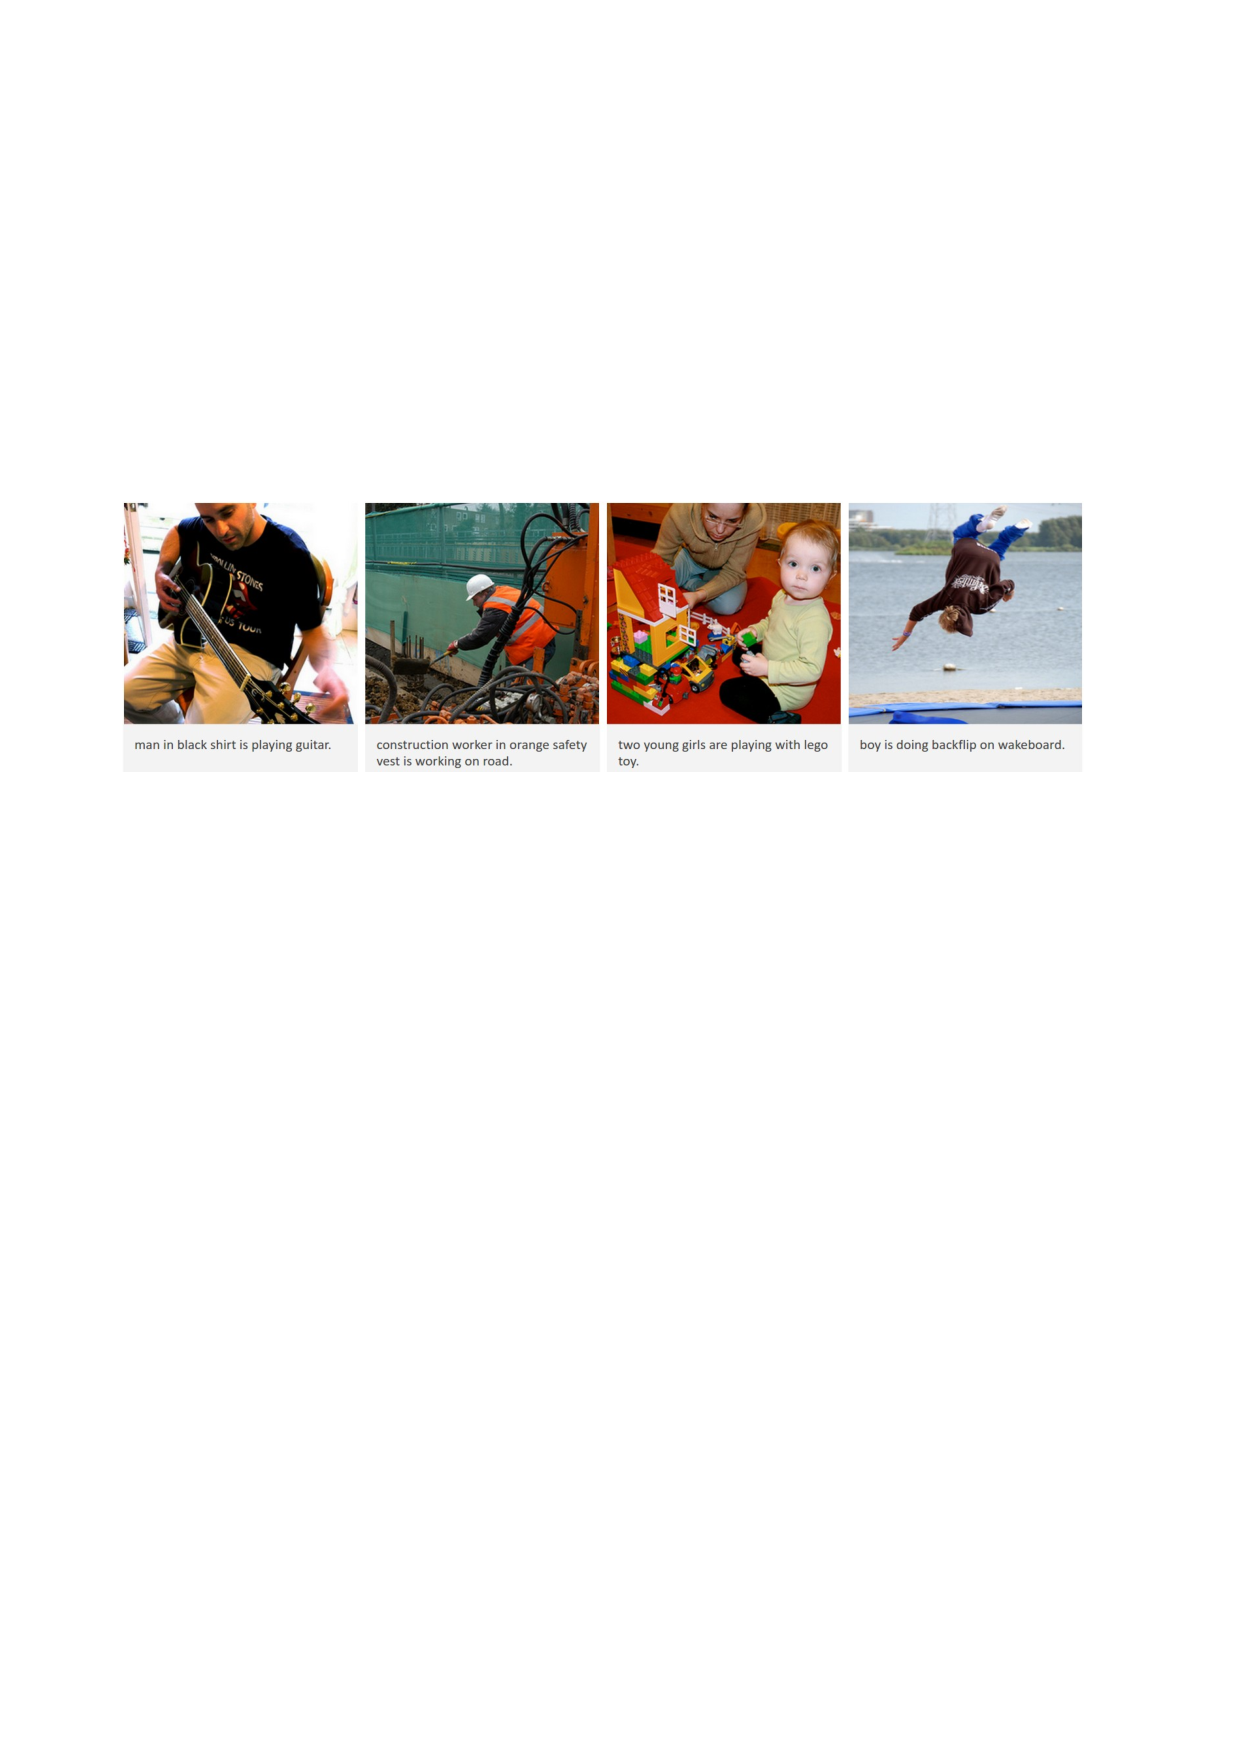
\includegraphics[width=\textwidth]{ImageCaptioning_1}}
  {
  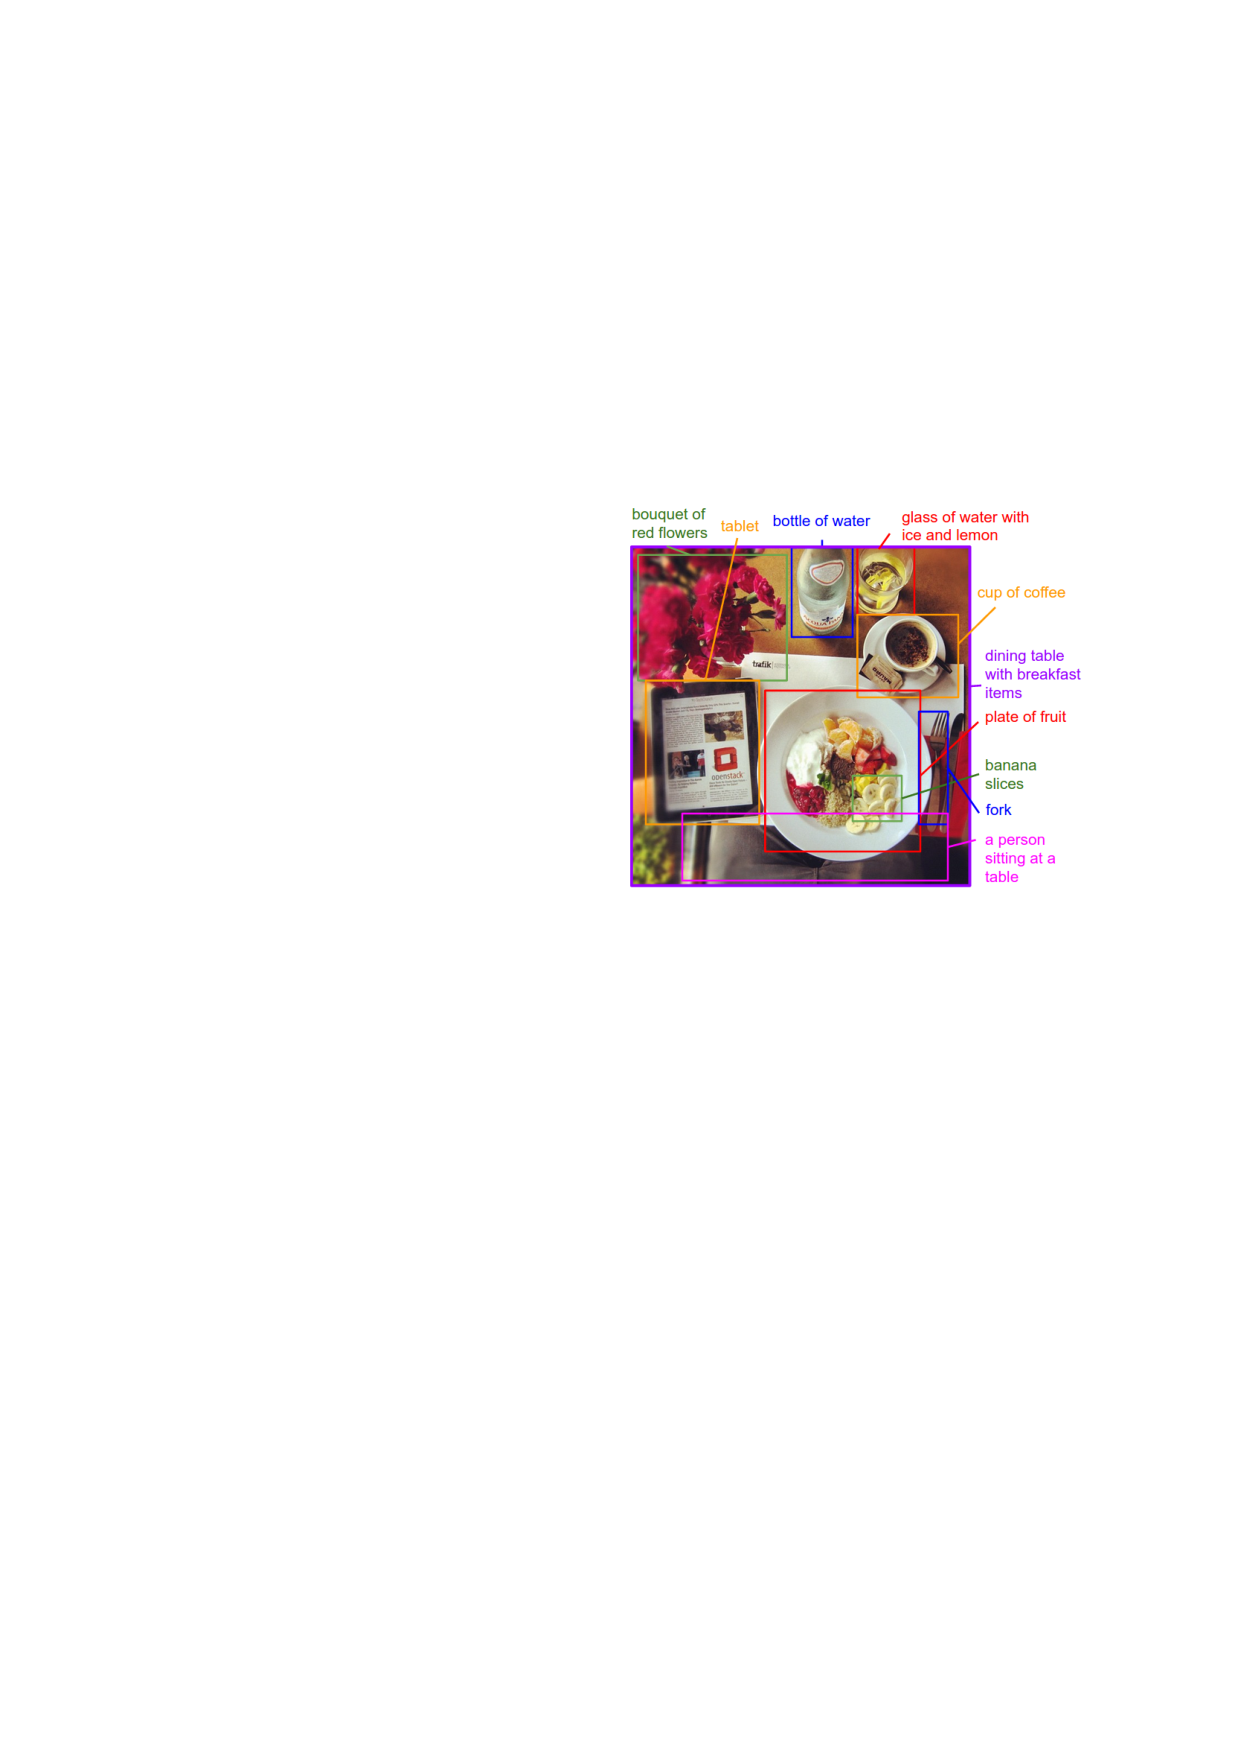
\includegraphics[height=0.75\textheight]{ImageCaptioning_2}
  \hfill
  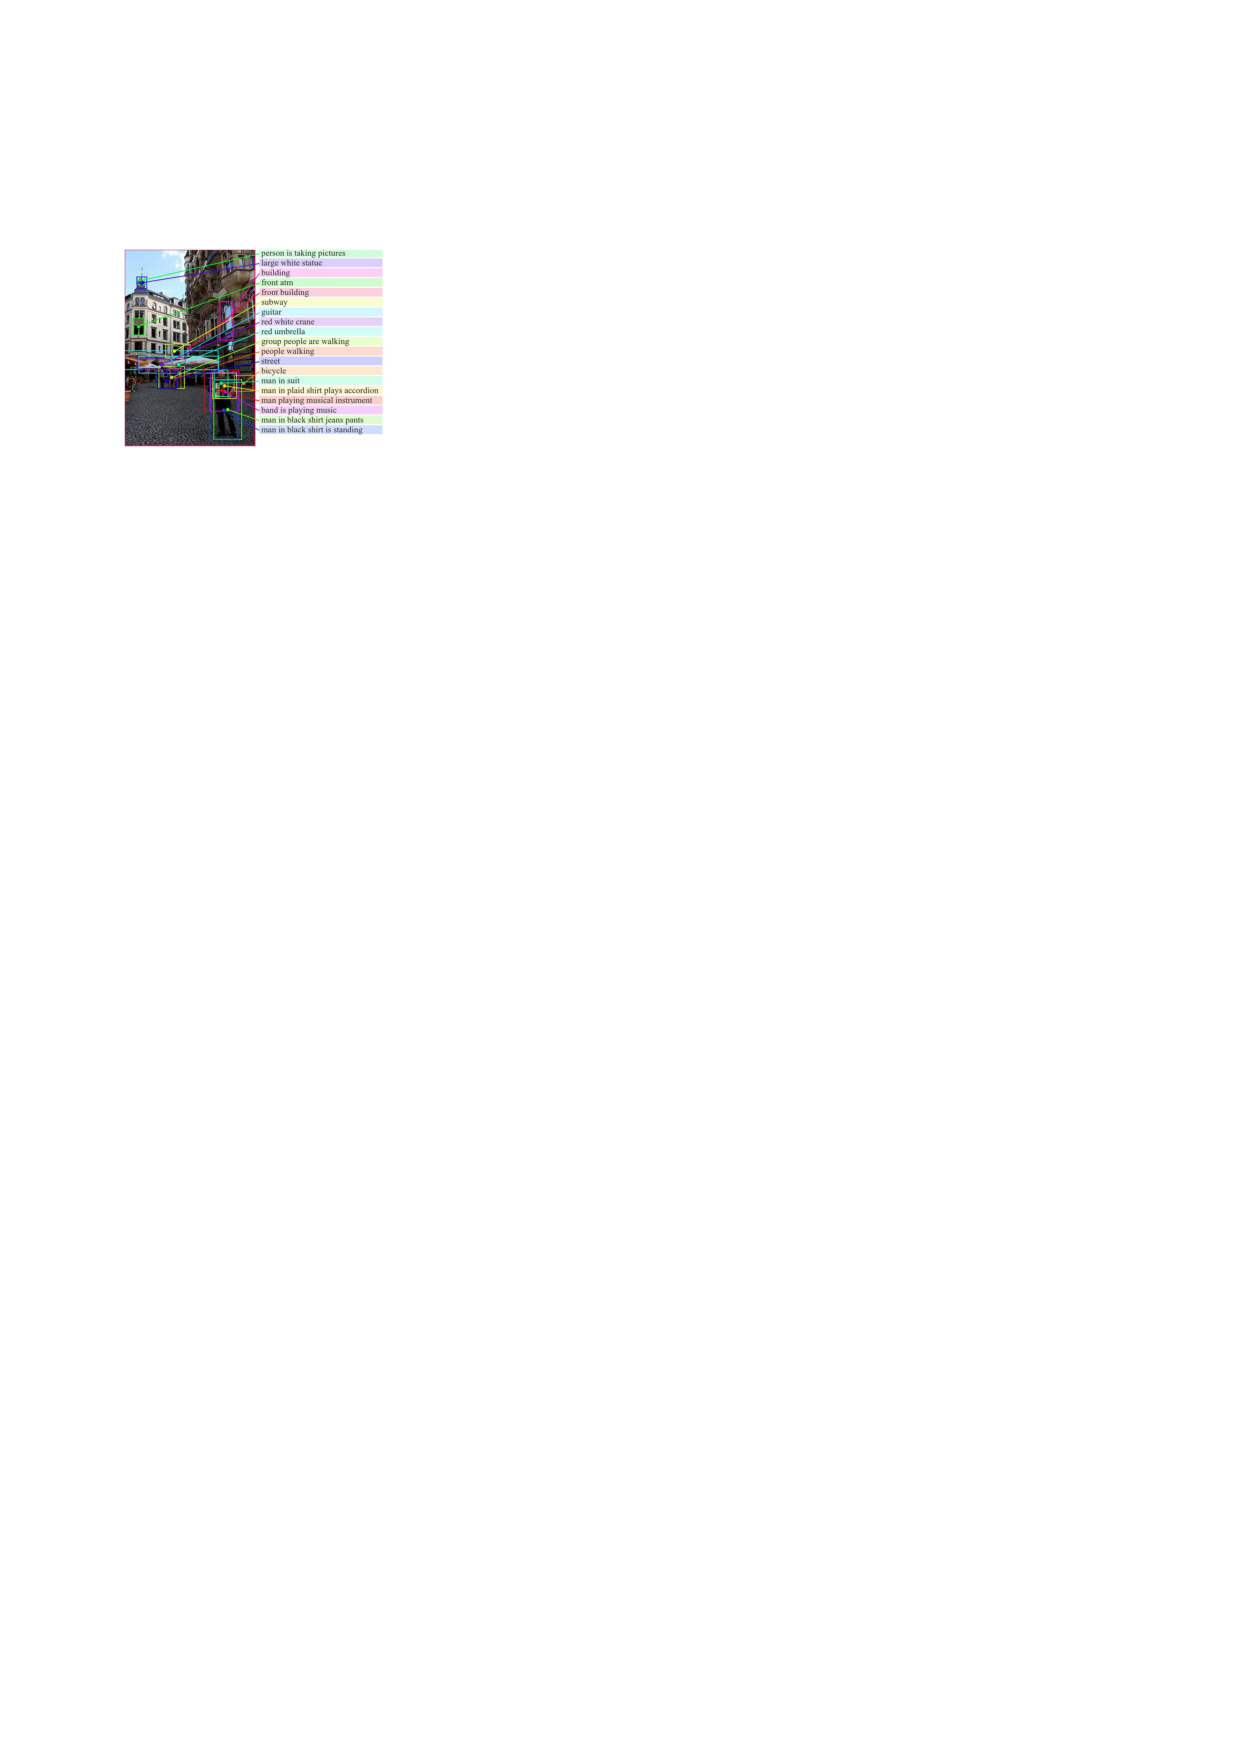
\includegraphics[height=0.75\textheight]{ImageCaptioning_3}
%  \hfill
%  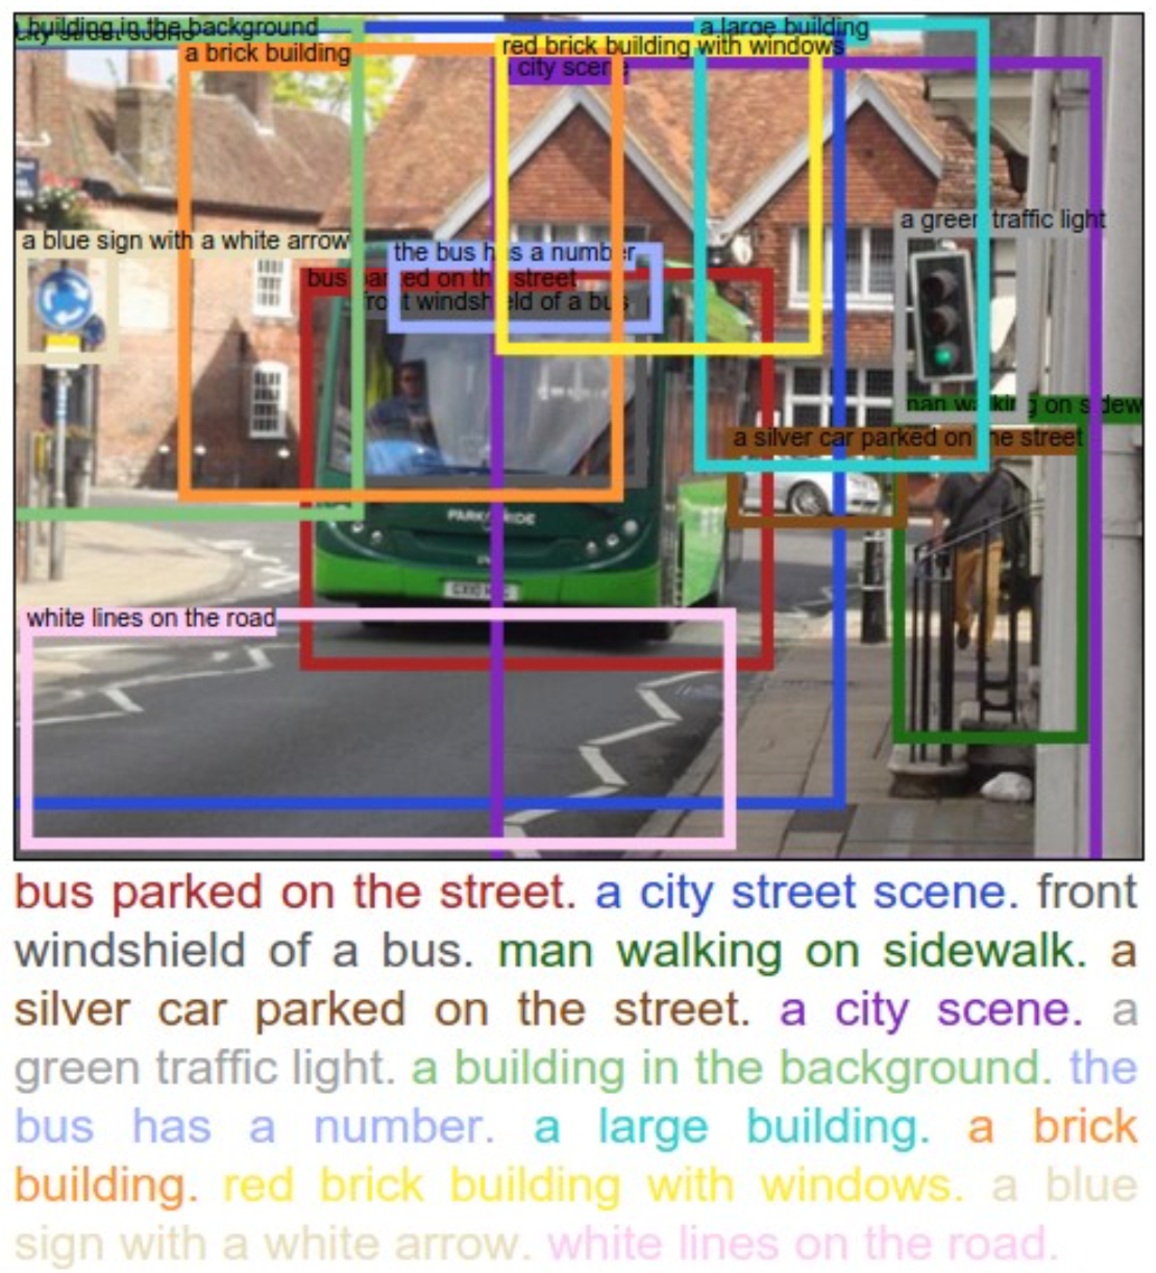
\includegraphics[width=0.3\textwidth]{ImageCaptioning_4}
  }
\onslide<6-7>
  \structure{Style transfer:} Transfer artistic style between art \cite{Gatys:2016aa} or photons \cite{Luan:2017aa}.
  \par\medskip
  \alt<6>{%
  \begin{columns}
  \begin{column}{0.5\textwidth}
    \centering
    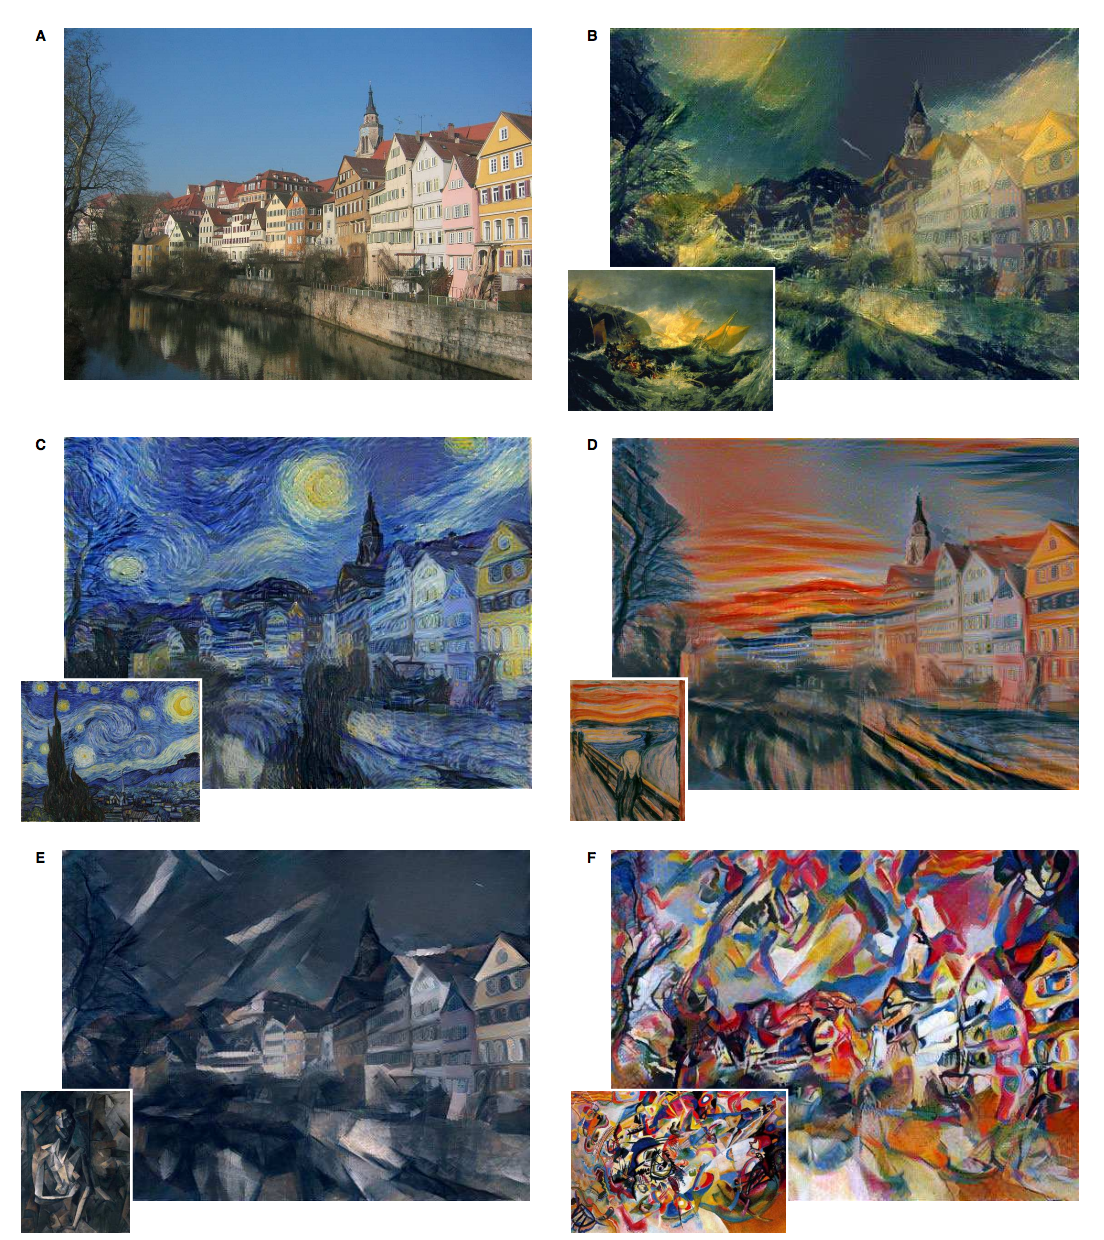
\includegraphics[height=0.7\textheight]{StyleTransfer}
  \end{column}
  \begin{column}{0.5\textwidth}
    \centering
    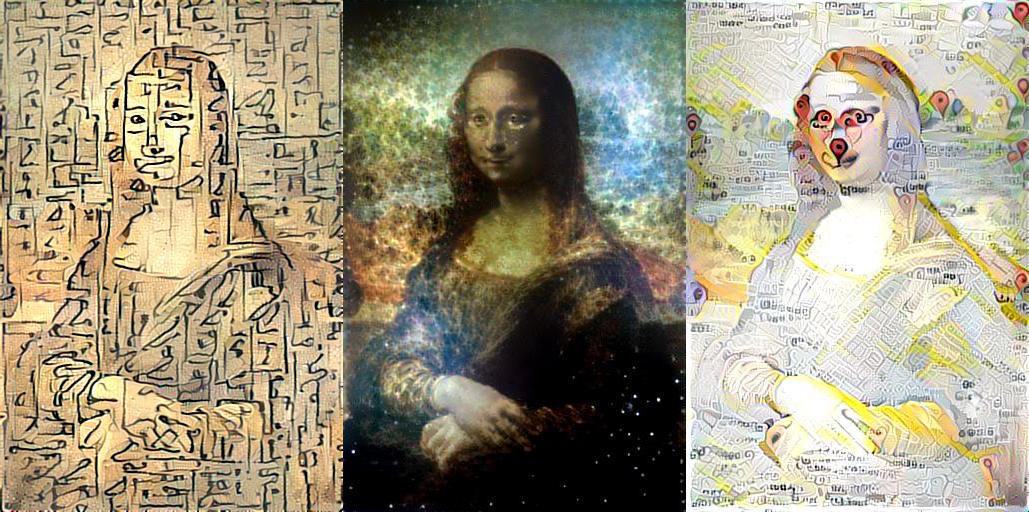
\includegraphics[width=\textwidth]{StyleTransfer2}  
  \end{column}
  \end{columns}
  }{%
  \par \begin{center}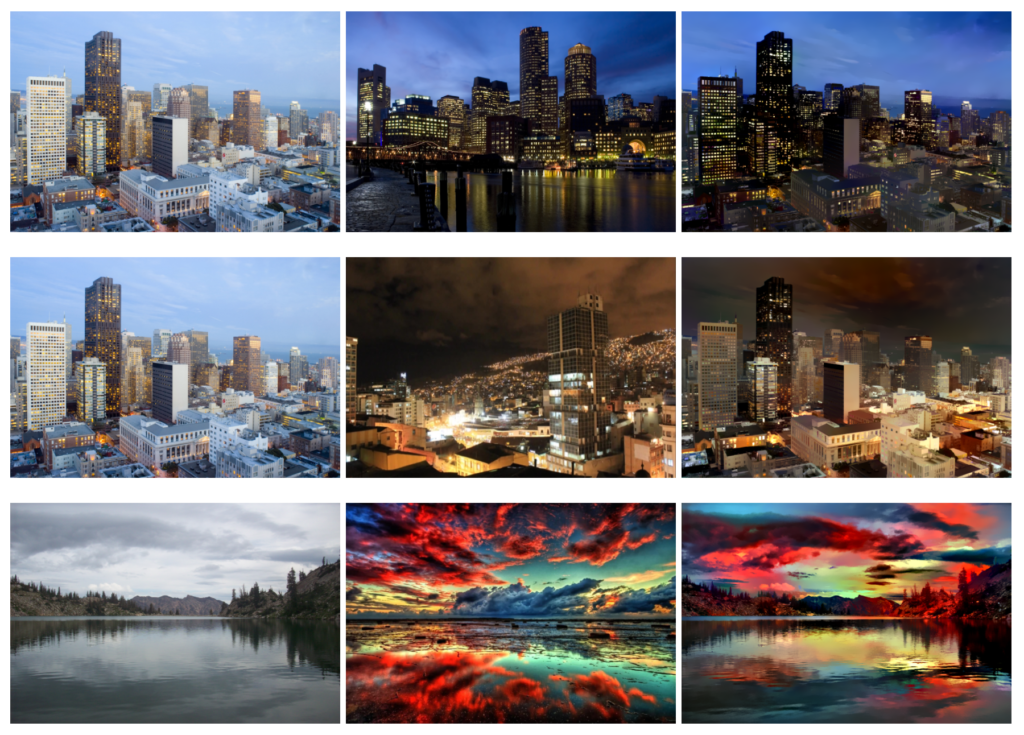
\includegraphics[height=0.7\textheight]{Photo_style_transfer}\end{center}
  }
\onslide<8>  
  \structure{Language translation:} Translate between languages \cite{Wu:2016aa}.
  \par\medskip
  \begin{columns}
  \begin{column}{0.5\textwidth}
    \centering
      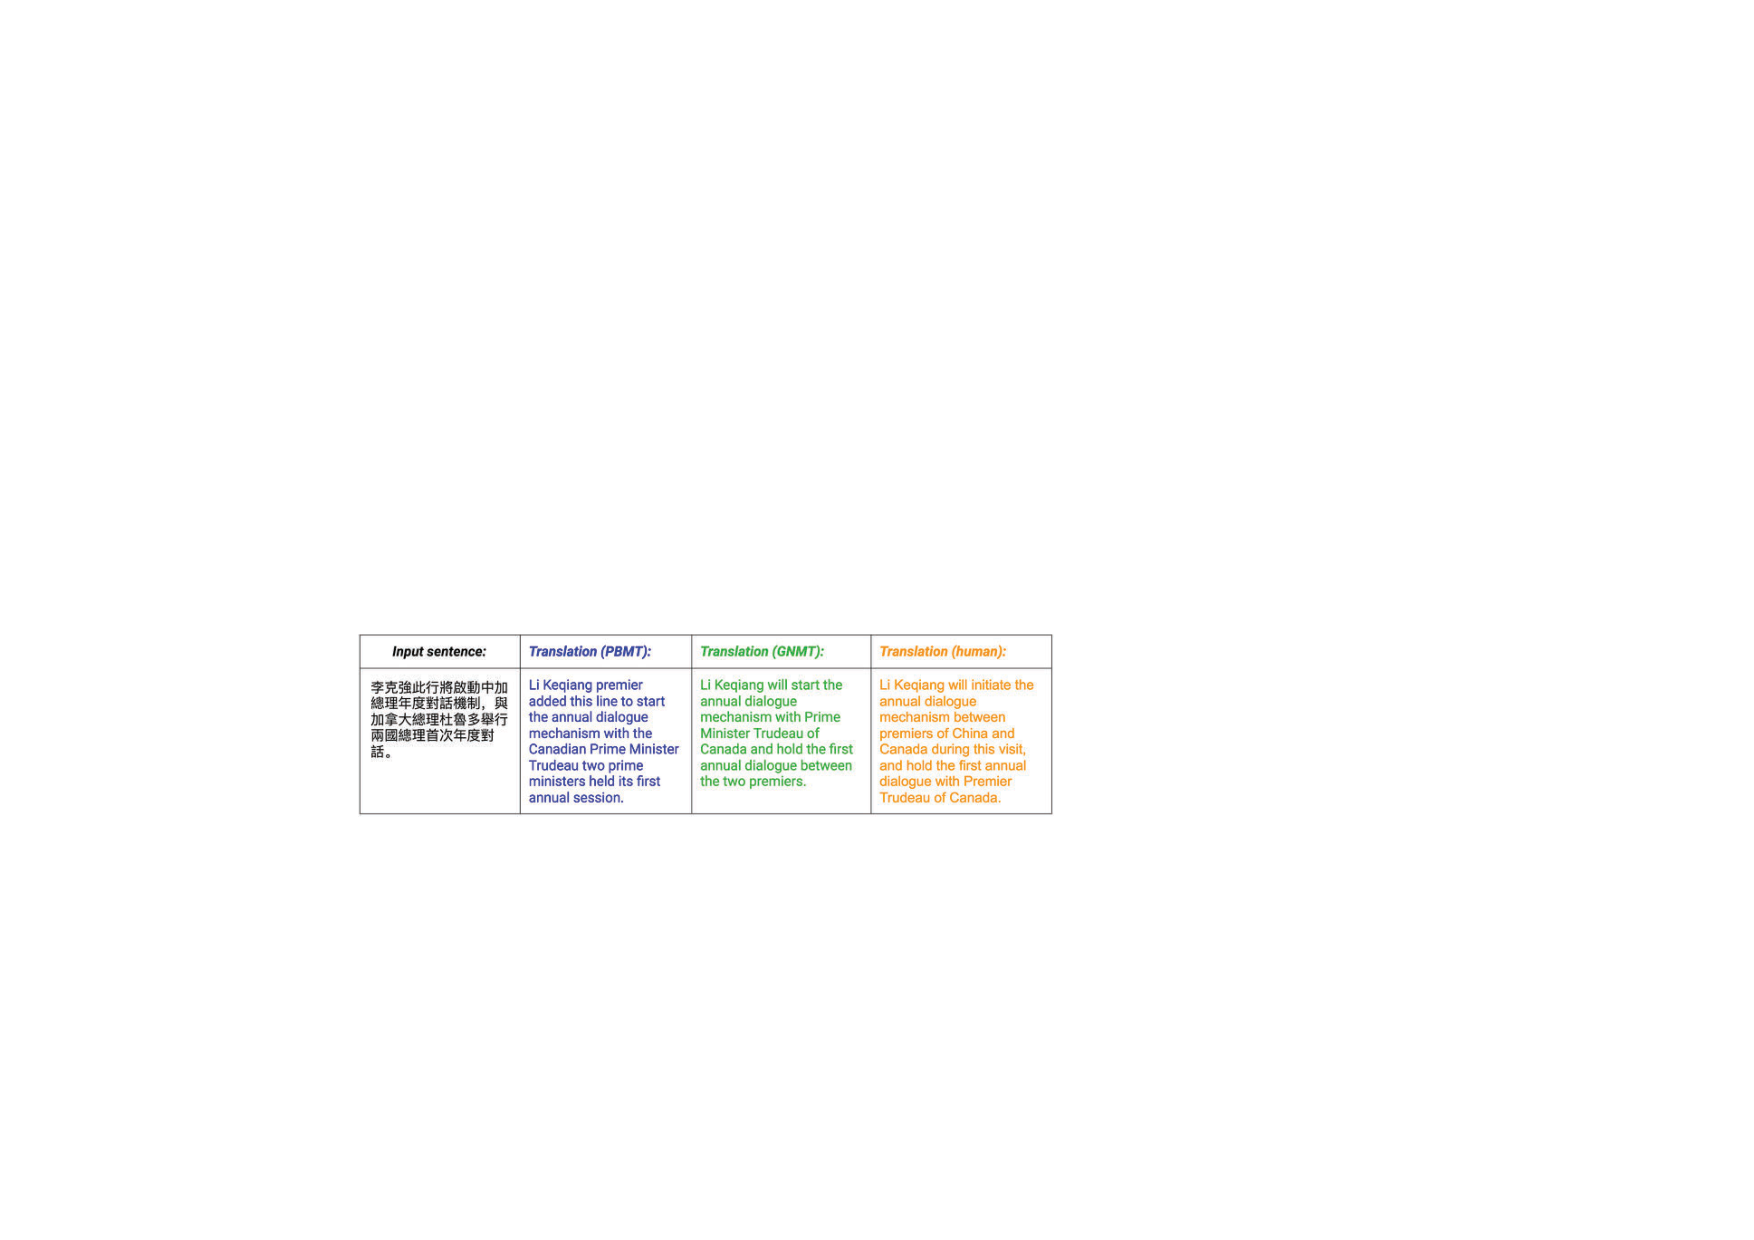
\includegraphics[width=\textwidth]{MachineTranslationExample}
      \par\bigskip
      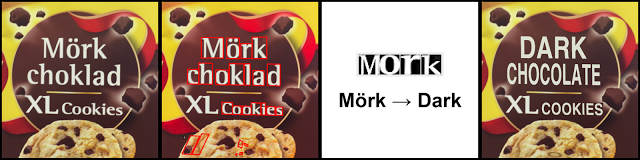
\includegraphics[width=\textwidth]{MachineTranslationExample2}      
  \end{column}
  \begin{column}{0.4\textwidth}
    \centering
    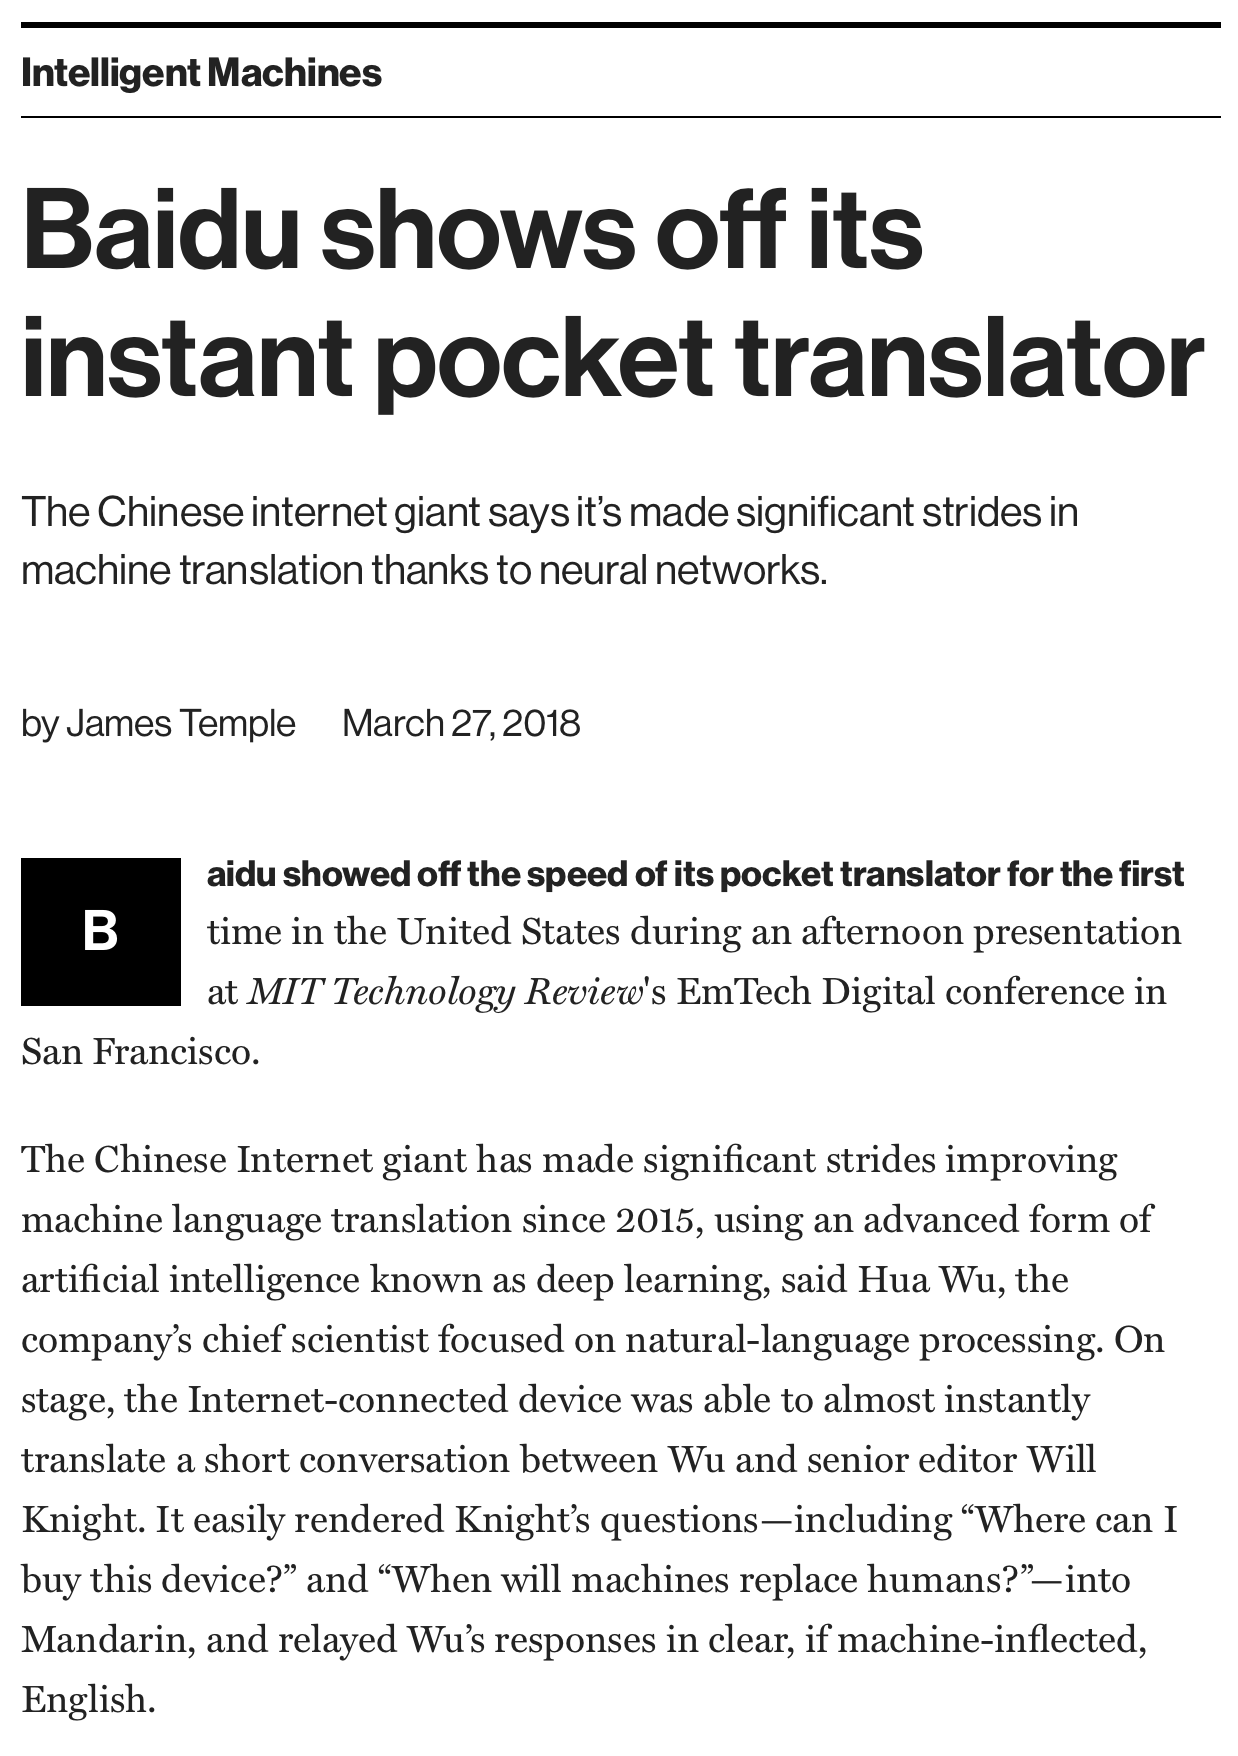
\includegraphics[height=0.8\textheight]{MachineTranslationNews}
  \end{column}
  \end{columns}
\onslide<9>
  \structure{Self-driving vehicles:} Drive vehicle safely and efficiently to destination 
  \begin{center}
  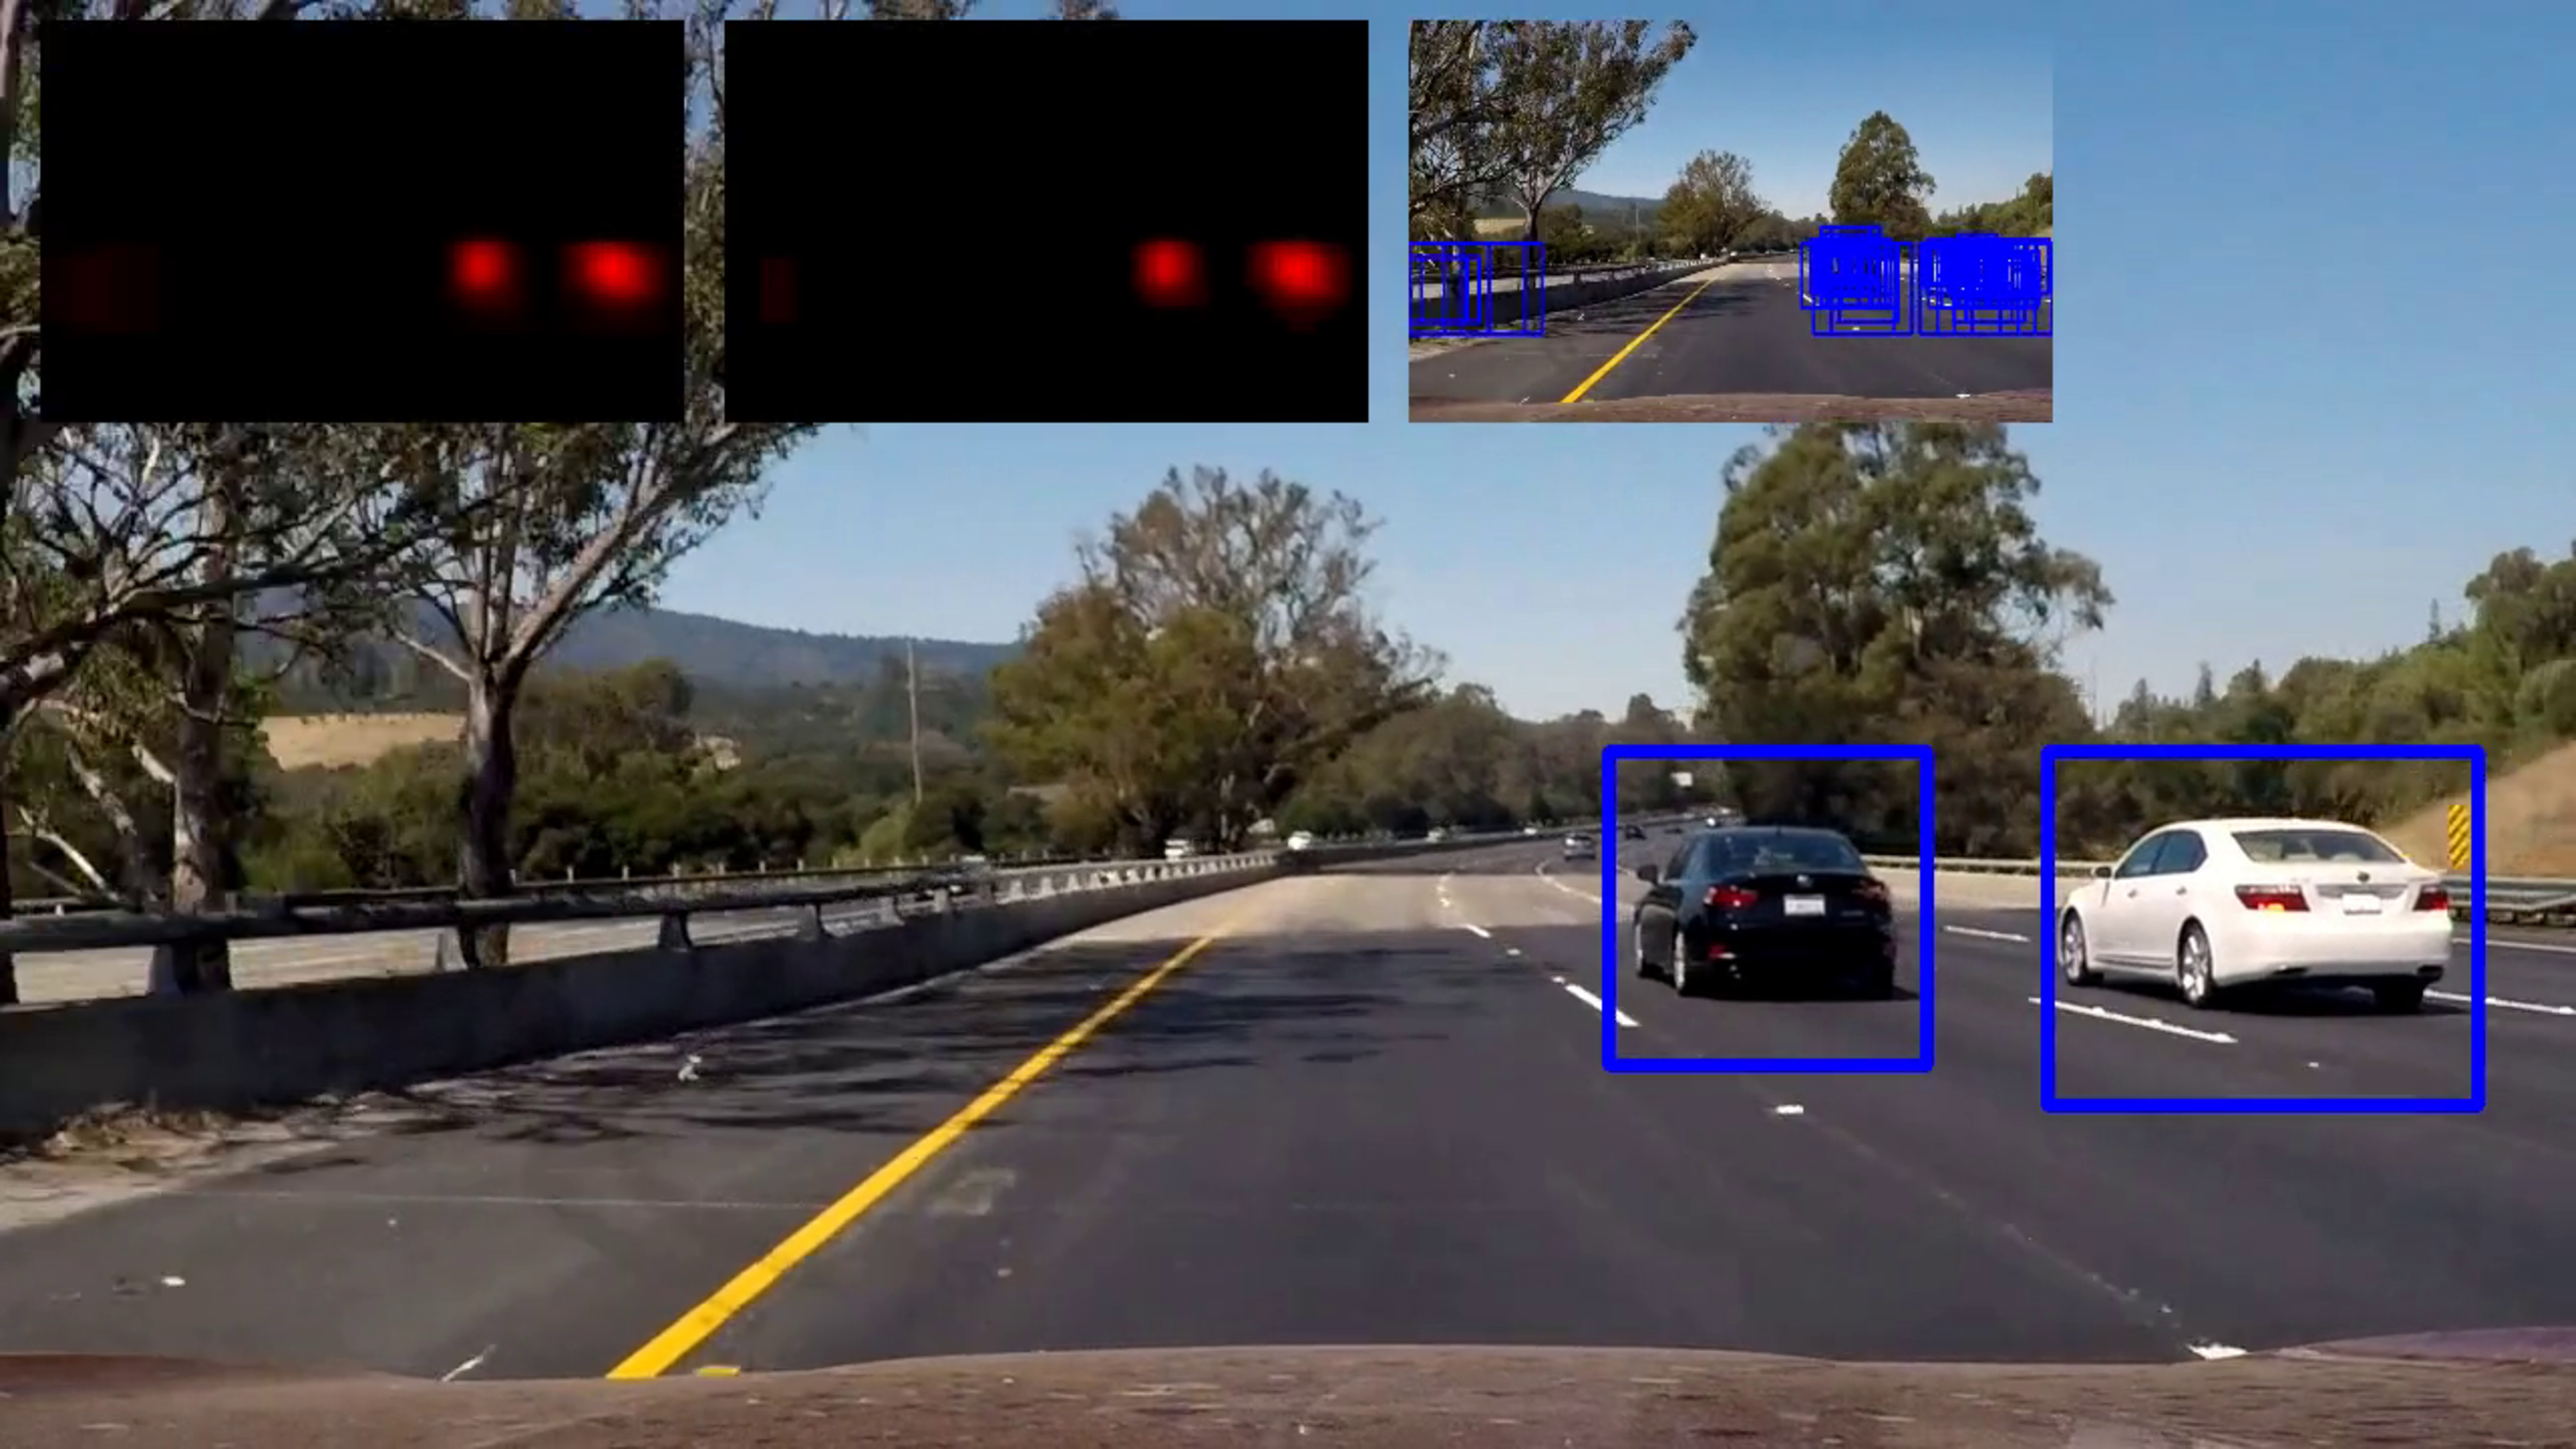
\includegraphics[width=0.75\textwidth]{Self-drivingCar}
  \end{center}
\onslide<10>
  \structure{Games:} Jeopardy \cite{Ferrucci:2013aa}, Go \cite{Silver:2016aa}, Poker \cite{Moravcik:2017aa}, video games \cite{Mnih:2015aa}, \ldots
  \par\medskip
  \begin{columns}[T]
  \begin{column}{0.3\textwidth}
    \centering
    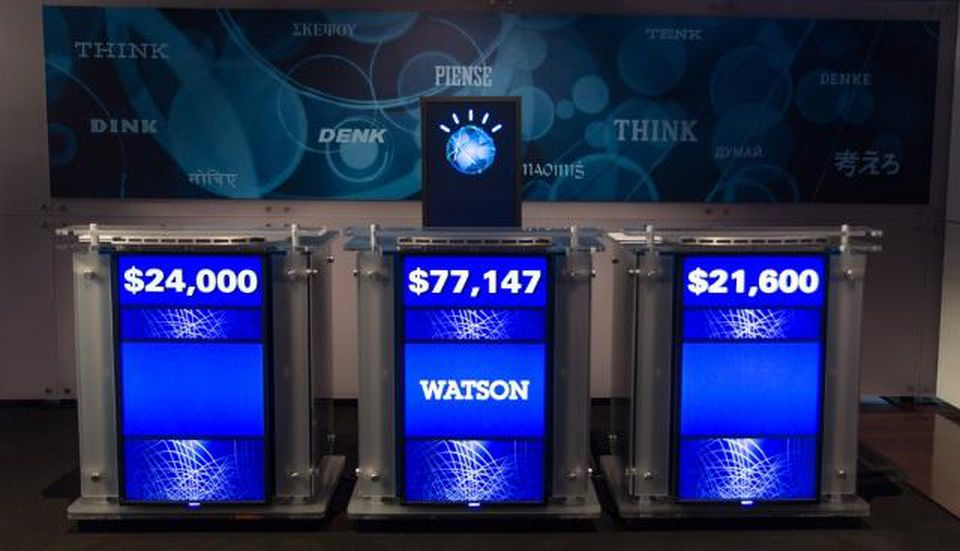
\includegraphics[width=\textwidth]{Watson}
    \par Jeopardy
    \end{column}
  \begin{column}{0.3\textwidth}
    \centering
    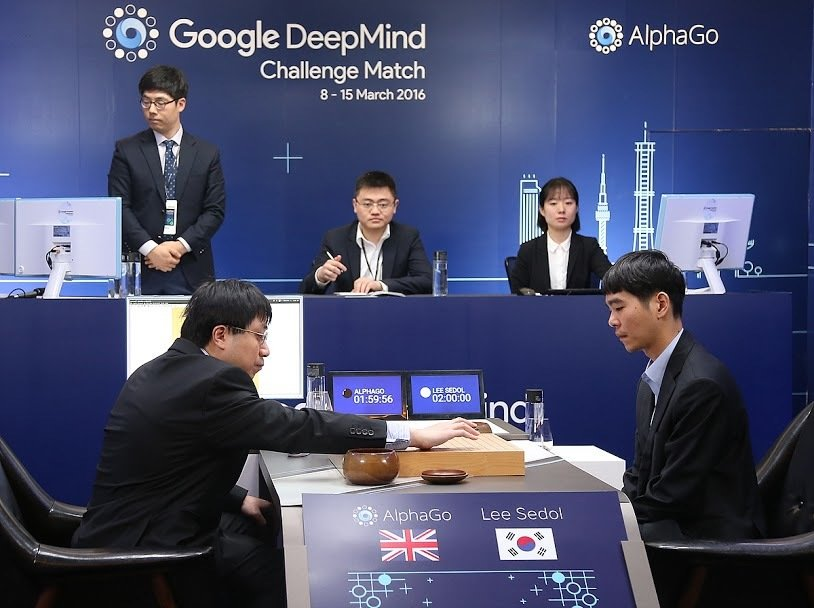
\includegraphics[width=\textwidth]{AlphaGo}  
    \par Go
  \end{column}
  \begin{column}{0.3\textwidth}
    \centering
    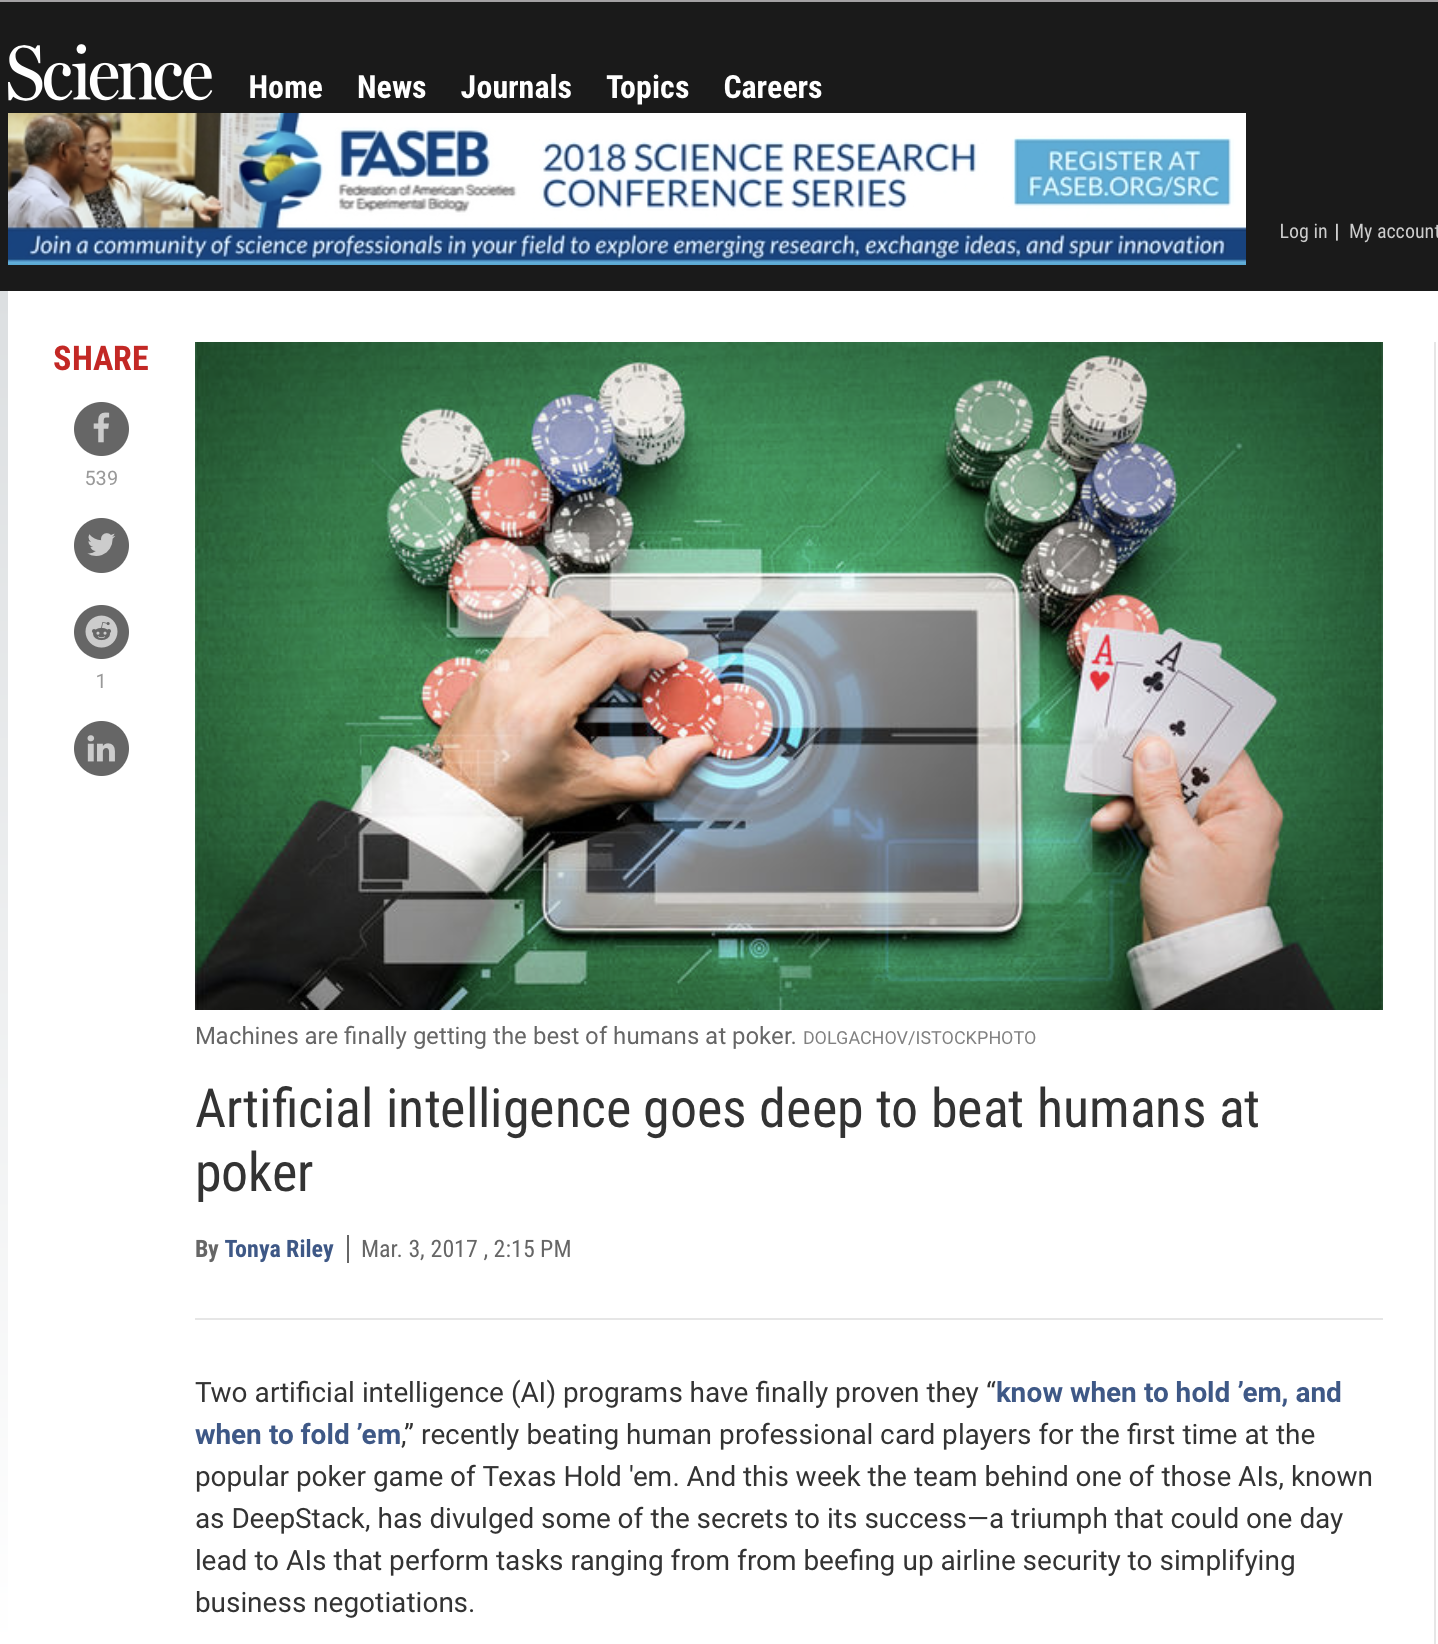
\includegraphics[width=\textwidth]{PokerNews}  
    \par Poker
  \end{column}
  \end{columns}
%  \begin{columns}[T]
%  \begin{column}{0.35\textwidth}
%    \raggedleft
%    Video games
%  \end{column}
%  \begin{column}{0.65\textwidth}
%     \raggedright
%     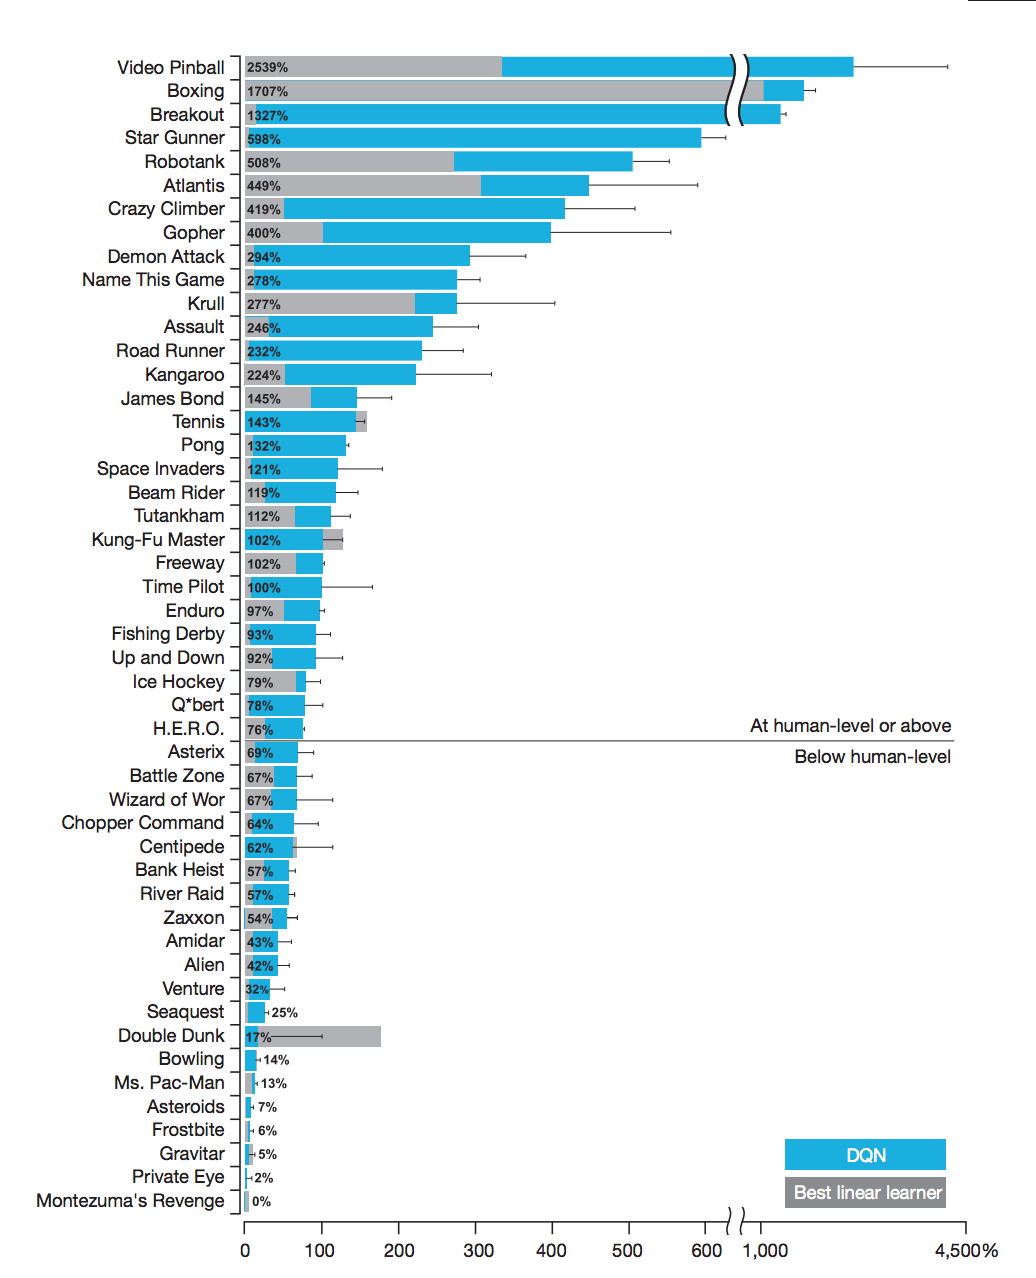
\includegraphics[height=0.75\textheight]{GamesChart}
%  \end{column}
%  \end{columns}    
\onslide<11>  
\structure{Current status}
\begin{itemize}
\item Deep learning currently addresses many tasks with unsurpassed results.
\item \structure{Key aspects behind success stories} 
\begin{itemize}
  \item Many network layers \& huge amount of training data.
  \item Massively parallelised hardware accelerated (GPU, TPU, \ldots) implementations.
  \item Optimisation algorithms for learning that regularise (stochastic gradient descent combined with effective initialisation, pooling, Dropout, \ldots). 
\end{itemize}
\item Little theoretical understanding, e.g., the optimisation for learning is highly non-convex and seems intractable from a theoretical viewpoint.
\item Success stories mostly confined to tasks where knowledge about how data is generated is not necessary, or has little importance.
\end{itemize}
\end{overprint}
\end{frame}

% Frame
\begin{frame}{But all is not well \ldots}
\begin{columns}[T]
\begin{column}{0.3\textwidth}
  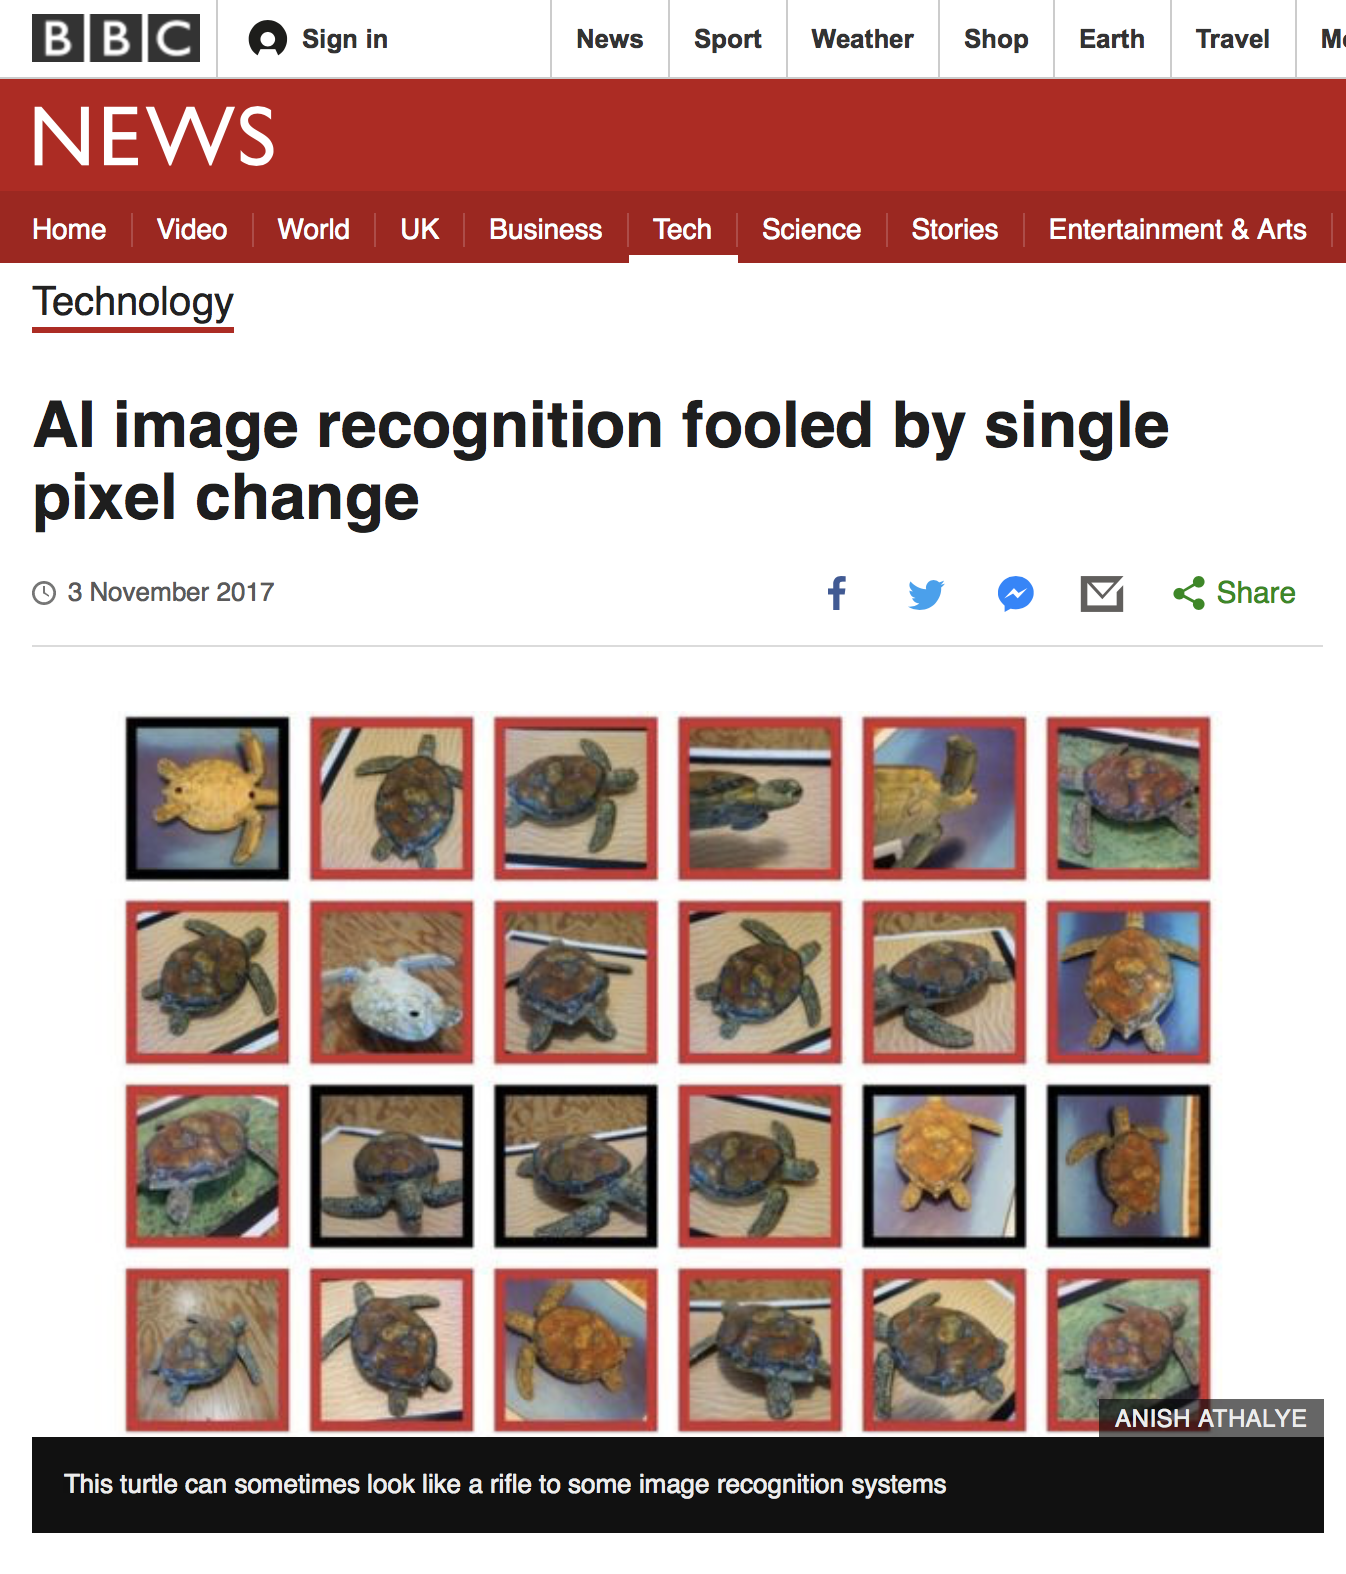
\includegraphics[width=\textwidth]{Missclassification}
\end{column}
\begin{column}{0.3\textwidth}
  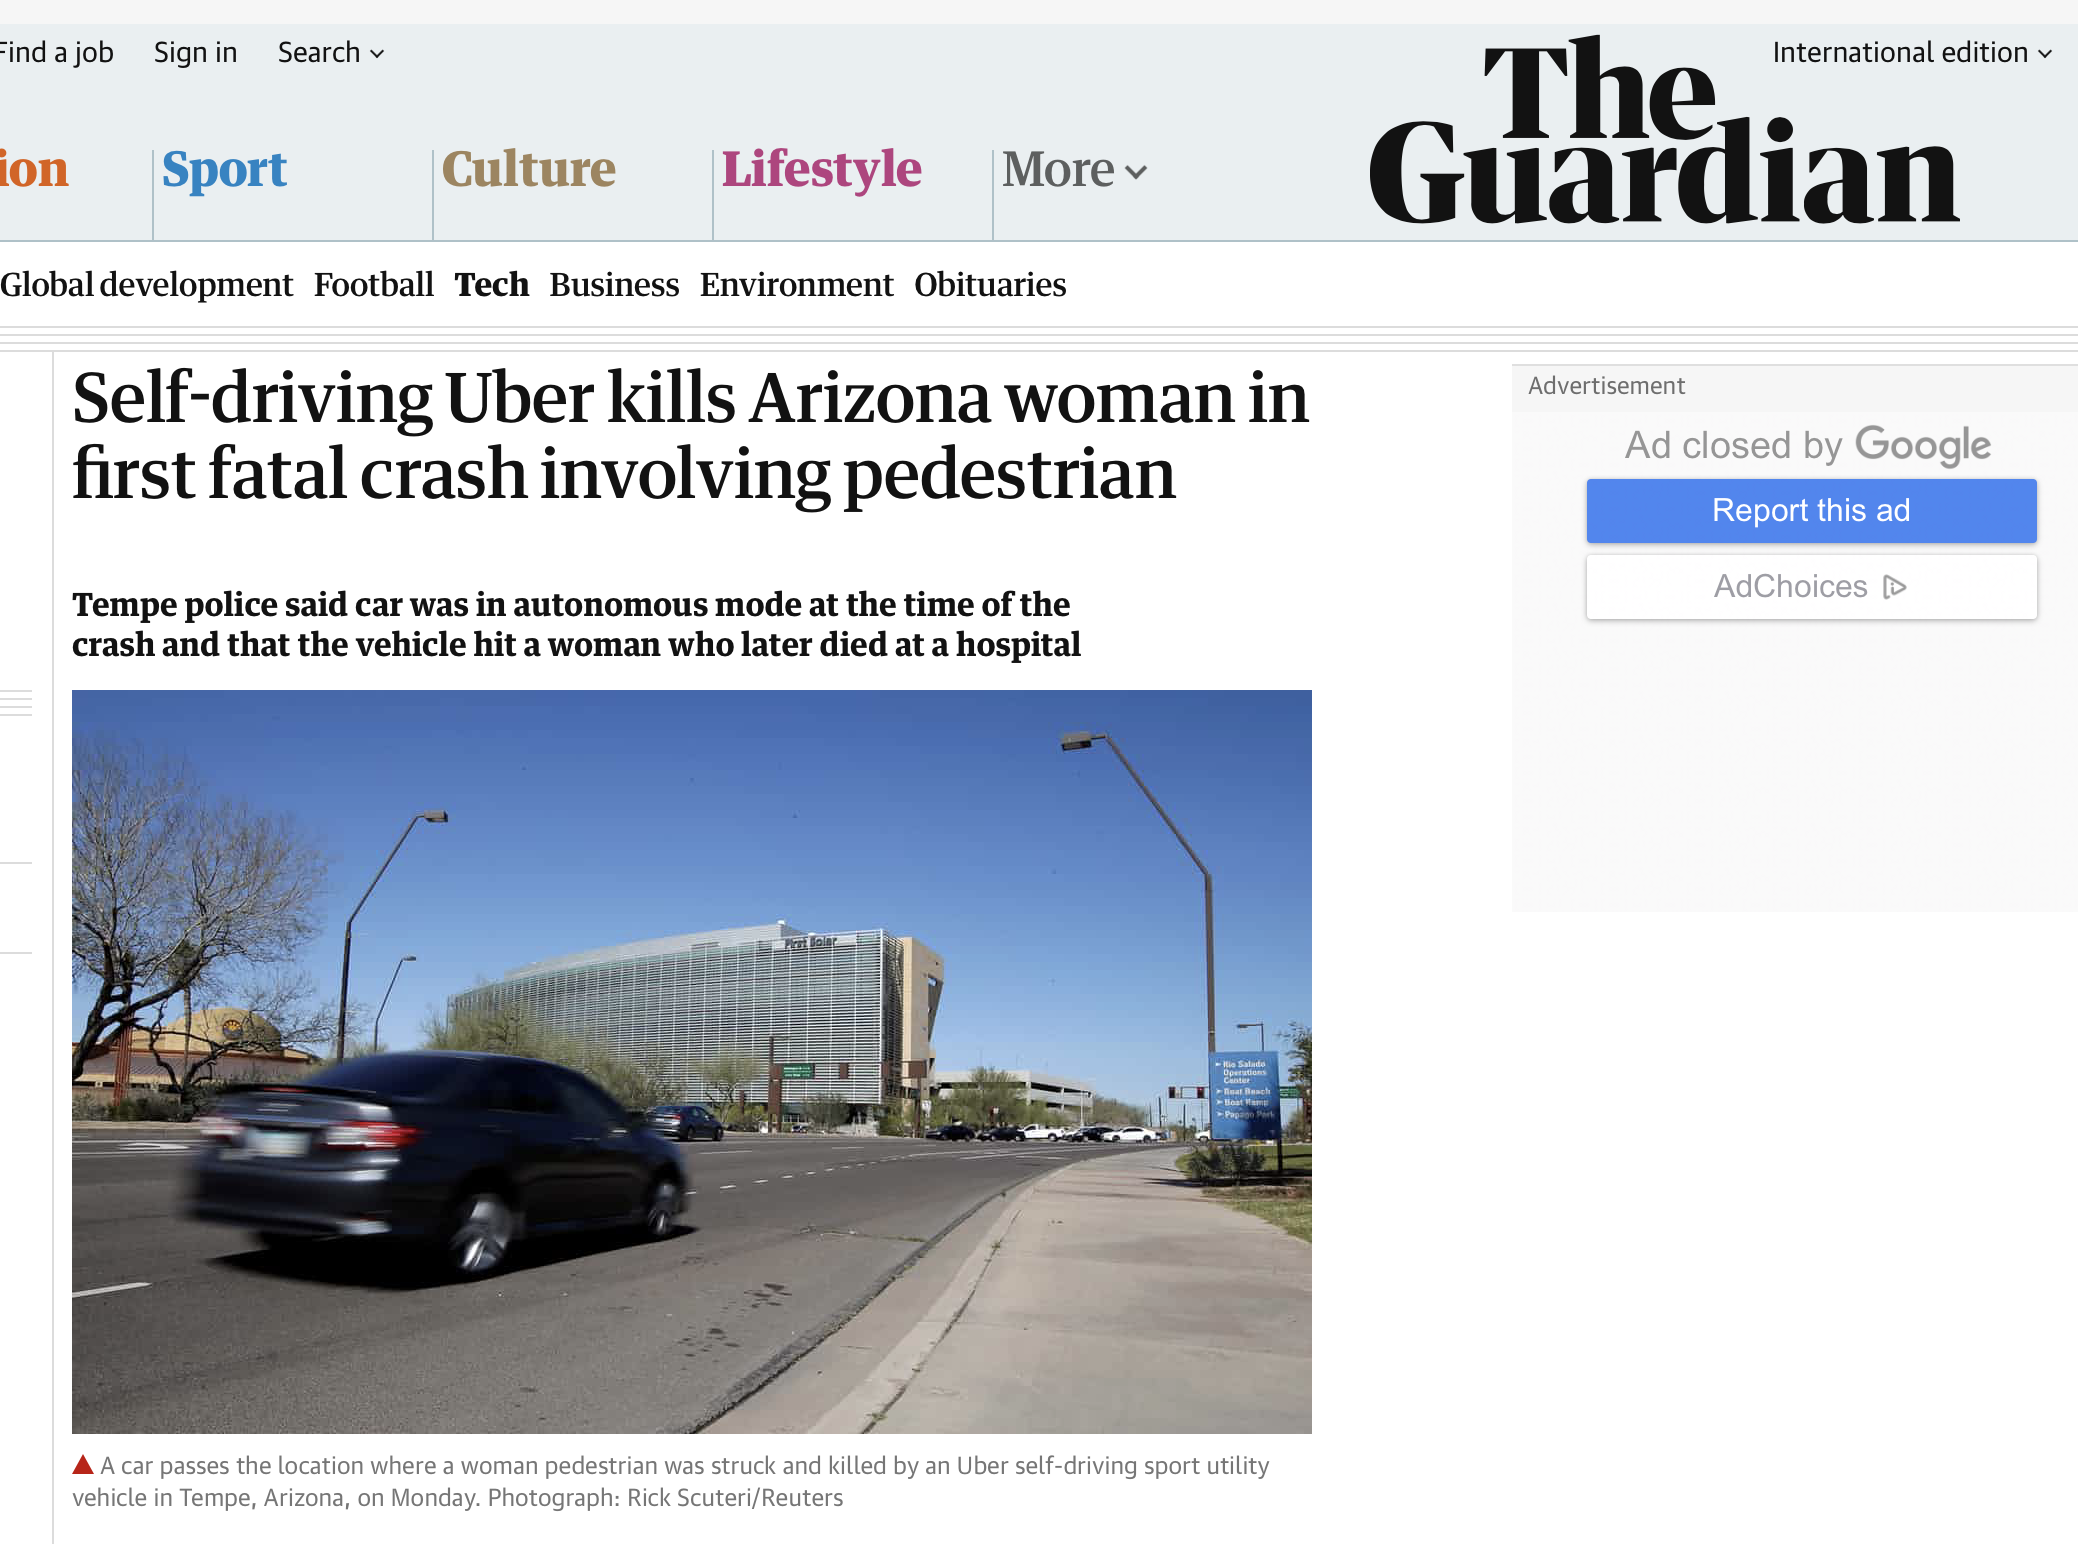
\includegraphics[width=\textwidth]{Selfdriving_accident}
\end{column}
\begin{column}{0.3\textwidth}
  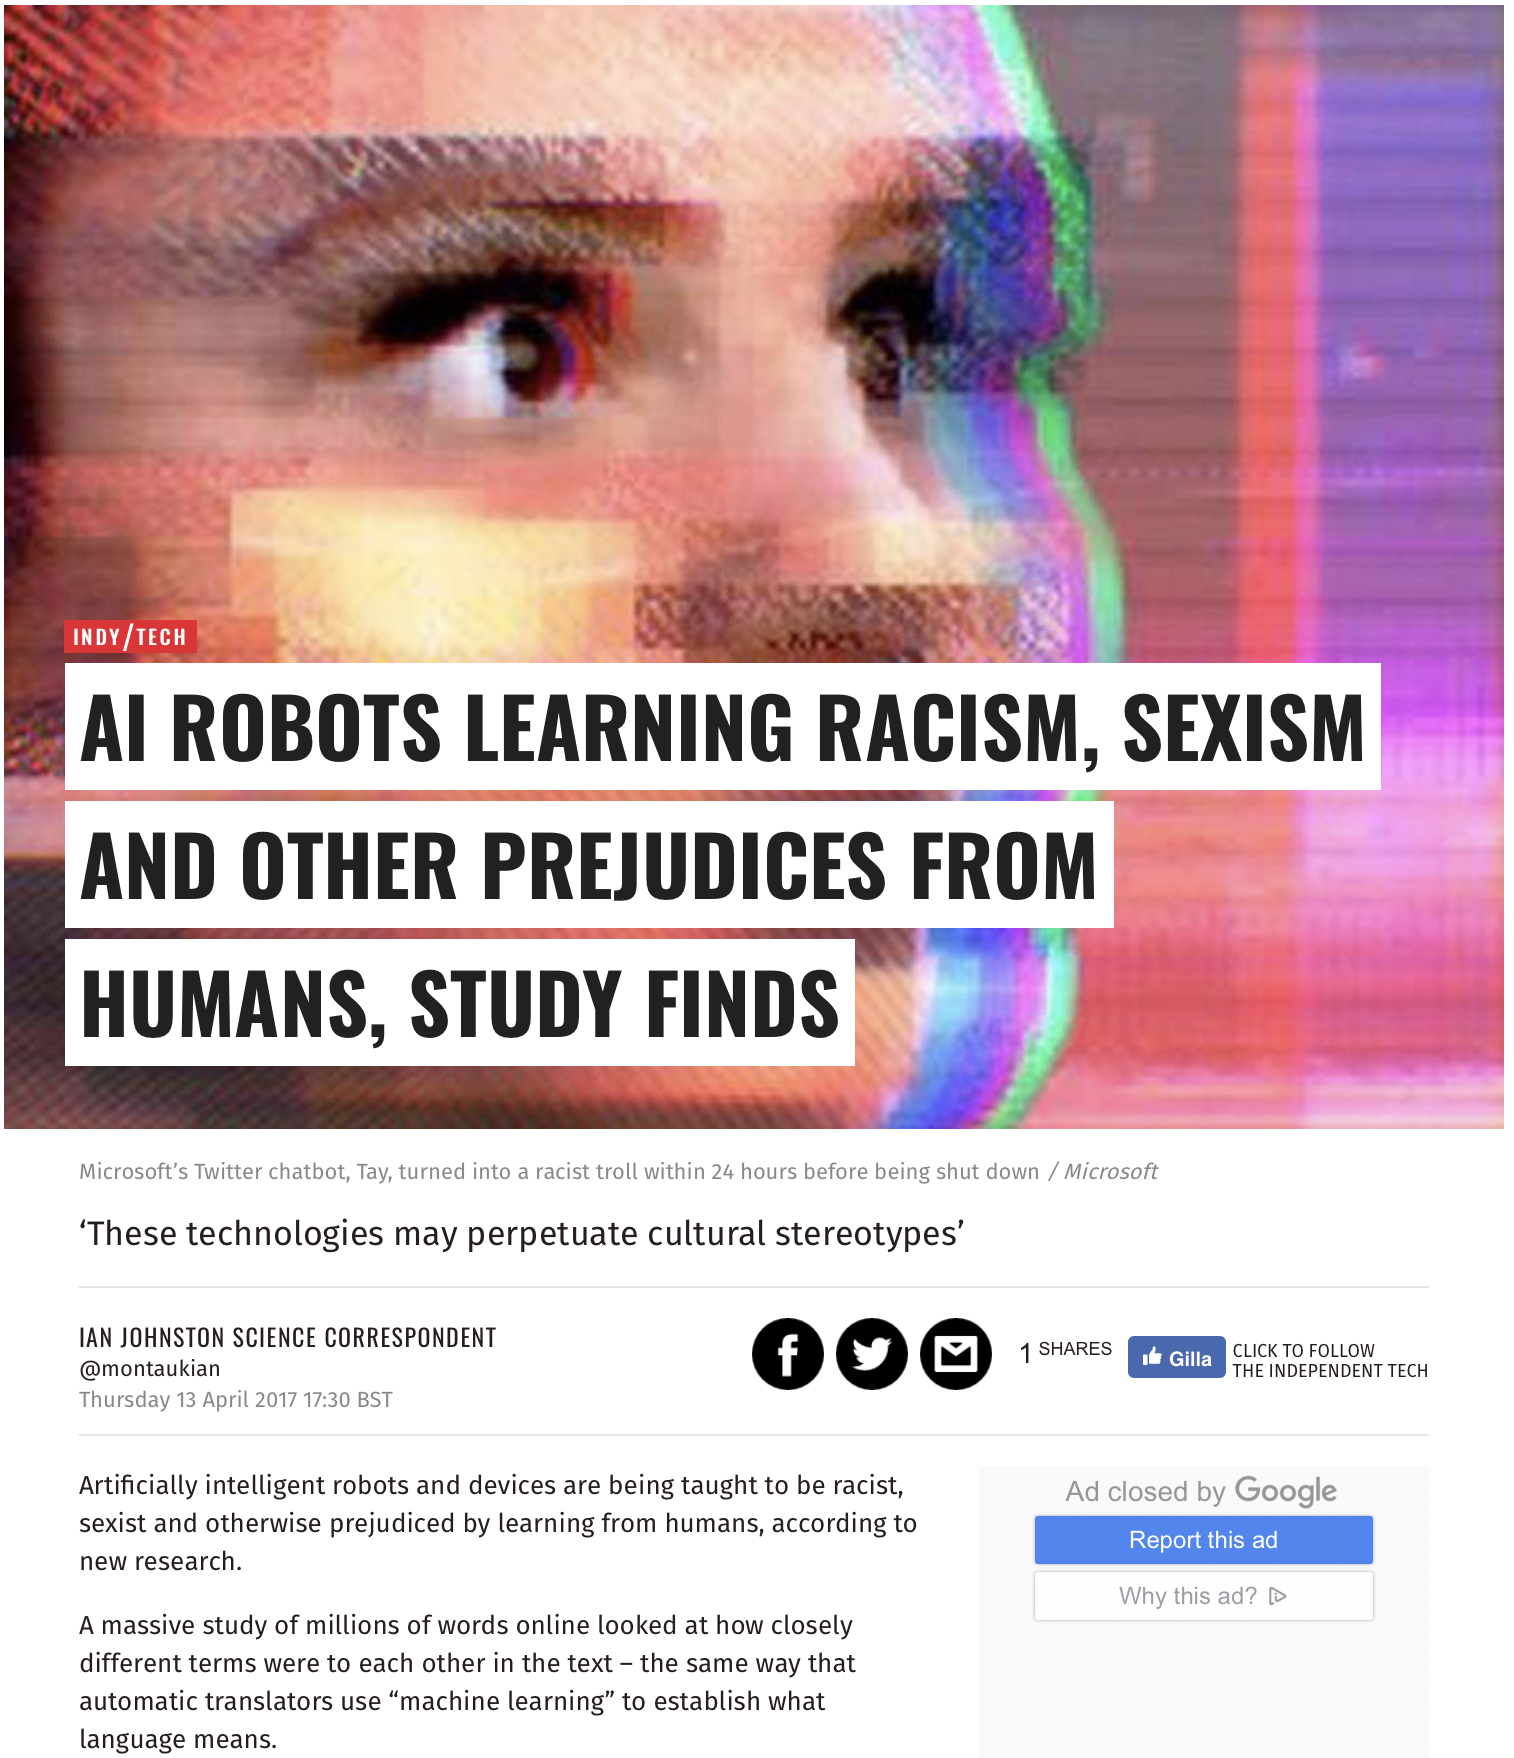
\includegraphics[width=\textwidth]{AI_bot_racist}
\end{column}
\end{columns}
\centering
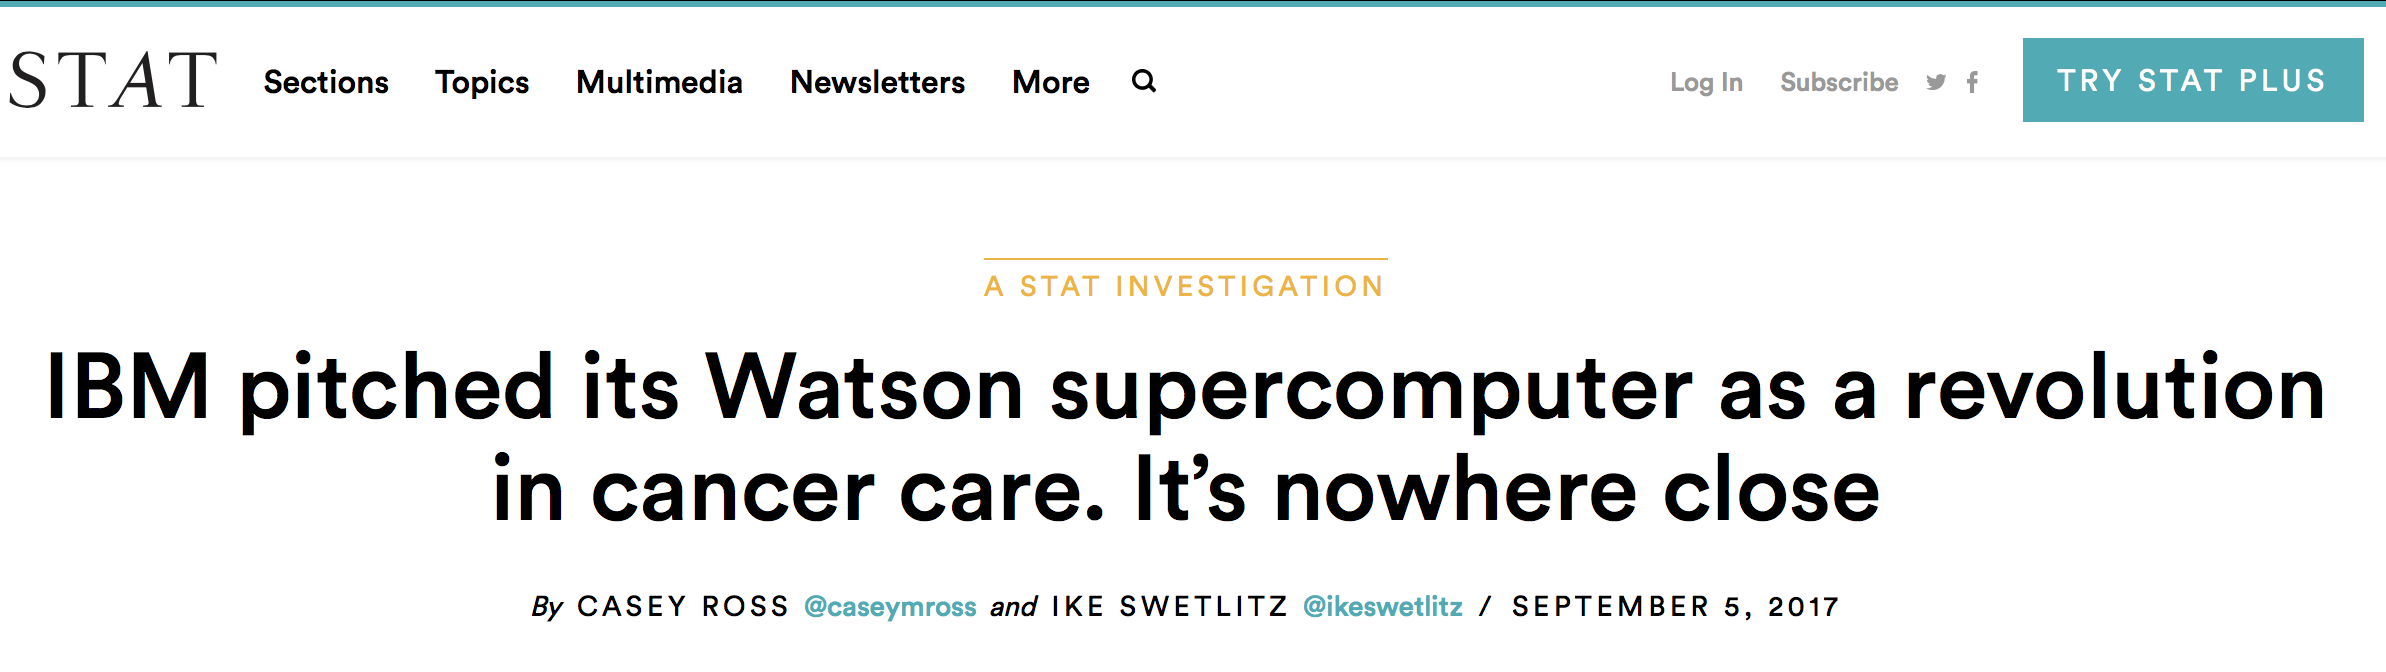
\includegraphics[height=0.3\textheight]{Watson_Oncology_1}
\end{frame}


% Frame
\begin{frame}[plain]
\slideTitle{Statistical setting}
\begin{itemize}
\item Supervised learning
\item Unsupervised and reinforcement learning
%\item Statistical models 
\end{itemize}
\end{frame}


% Frame
\begin{frame}{Supervised learning}
\begin{itemize}
\item \structure{Task:} 
Determine measurable map $\model \colon \InputSpace \to \OutputSpace$ from (supervised) training 
data $(\inputvar_i,\outputvar_i) \in \InputSpace \times \OutputSpace$, which are samples of a 
$(\InputSpace \times \OutputSpace)$-valued random variable $(\stinputvar,\stoutputvar)$ such that 
$\model(\stinputvar) \approx \stoutputvar$. 
%\item \structure{Layman's formulation:} 
%  Find algorithm that models input-output relation from examples.
\item Neither the joint law of $(\stinputvar,\stoutputvar)$ nor any of the marginals are known.
\visible<2->{
\item \structure{Basic notions:} 
  \begin{itemize}
  \item Elements in $\InputSpace$: Input, features, or observed.
  \item Elements in $\OutputSpace$: Output, labels, or targets.
  \item The map $\model$: Model or hypothesis.
  \item Learning/training algorithm: Procedure for estimating $\model$ from training data.
  \end{itemize}
\item \structure{Generic (fully data driven) setting:} No other additional information beyond what is contained in training data.
}
\visible<3->{
\item \structure{Classification:} $\OutputSpace$ is a finite set.
\item \structure{Regression:} $\OutputSpace$ is (in most cases) a vector space.
\item \structure{Connection to statistical decision theory:}
\begin{itemize}
  \item Mappings from $\InputSpace$ to $\OutputSpace$ represent (non-randomised) decision rules.
  \item Decision problem: Select `optimal' decision rule given training data.
\end{itemize}
}
\end{itemize}
\end{frame}

% Frame
\begin{frame}{Unsupervised and reinforcement learning}
\begin{itemize}
\item \structure{Unsupervised learning:}
Discovering patterns in data in the absence of either an identified output supervised learning or feedback (reinforcement learning).
\\[1em]
\structure{Examples:} Clustering, association rules, topological data analysis, and self-organising maps.
\\[2em]
\item \structure{Reinforcement learning:}
Learning based on feedback or reward, i.e., there are no input-output pairs indicating correct and incorrect outcome (unlike in supervised learning) but there is a reward (unlike unsupervised learning).
\\[1em]
\structure{Examples:} Learn to play games by winning or losing.
\end{itemize}
\end{frame}

% Frame
\begin{frame}{Statistical models}
\begin{itemize}
\item \structure{Discriminative (conditional) model}
\begin{itemize}
\item Learns the conditional probability distribution $\Prob(\stoutputvar \mid \stinputvar=\inputvar)$ without reference to $\Prob(\stinputvar,\stoutputvar)$, $\Prob(\stinputvar)$, or $\Prob(\stinputvar \mid \stoutputvar=\outputvar)$.
\item Approaches further categorised based on choice of risk minimising decision rule:
  \begin{itemize}
  \item Support vector machines
  % Learns a decision boundary that maximises the distance between samples of the two classes, given a kernel.
  \item Decision trees
  % Learns decision boundary by recursively partitioning the space to maximise the information gain.
  \item Neural networks
  \item \ldots
  \end{itemize}
\end{itemize}
\item \structure{Generative model:} Model of how the data is actually generated.
\begin{itemize}
\item Learns the joint probability distribution $\Prob(\stinputvar,\stoutputvar)$, or $\Prob(\stoutputvar)$ and $\Prob(\stinputvar \mid \stoutputvar=\outputvar)$.
\item Typically specified by probabilistic graphical models, which offer rich representations of the causal relations in training dataset.
\end{itemize}
\end{itemize}
% https://stats.stackexchange.com/questions/12421/generative-vs-discriminative
%Discriminative models also do not generally function for outlier detection, though generative models generally do. 
%Generative models are typically specified as probabilistic graphical models, which offer rich representations of the independence relations in the dataset. 
%Discriminative models do not offer such clear representations of relations between features and classes in the dataset. 
%Instead of using resources to fully model each class, they focus on richly modelling the boundary between classes. Given the same amount of capacity (say, bits in a computer program executing the model), a discriminative model thus may yield more complex representations of this boundary than a generative model.
\end{frame}



% Frame
\begin{frame}[plain]
\slideTitle{Neural network architectures}
\begin{itemize}
\item Single layer network
\item Sequential deep network
\item \Acfp{CNN} 
\item Residual, dense, and sparse networks
\item \Acfp{RNN} 
\item Activation functions
\item Further components of modern neural networks
\end{itemize}
\end{frame}

% Frame
\begin{frame}{Basic notions}
\begin{itemize}
\item \structure{Neural networks:} 
Parametrised family $\{ \model_{\param} \}_{\param}$ where $\model_{\param} \colon \InputSpace \to \OutputSpace$ is (non-linear) measurable map and $\InputSpace$ and $\OutputSpace$ are fixed sets. 
\item \structure{Architecture (model class):}
  Precise description of how $\param$ yields $\model_{\param} \colon X \to Y$.
\end{itemize}
\end{frame}

% Frame
\begin{frame}{Single layer network (perceptron/artificial neuron)}
$\model_{\param} \colon \Real^n \to \Real^m$ non-linear measurable map given as $\model_{\param} := \NonLinMap \circ \LinMap_{\param}$ where:
\begin{itemize}
\item Affine linear map $\LinMap_{\param} \colon \Real^{n} \to \Real^{m}$ given by weights.
\item Point-wise non-linear map $\NonLinMap \colon \Real^{m} \to \Real^{m}$ given by $\Activation \colon \Real \to \Real$ (activation function).
\end{itemize}
\begin{columns}[T]
\begin{column}{0.55\textwidth} %% Column 1
\begin{overprint}
\onslide<2> % Slide 2
  \centering
  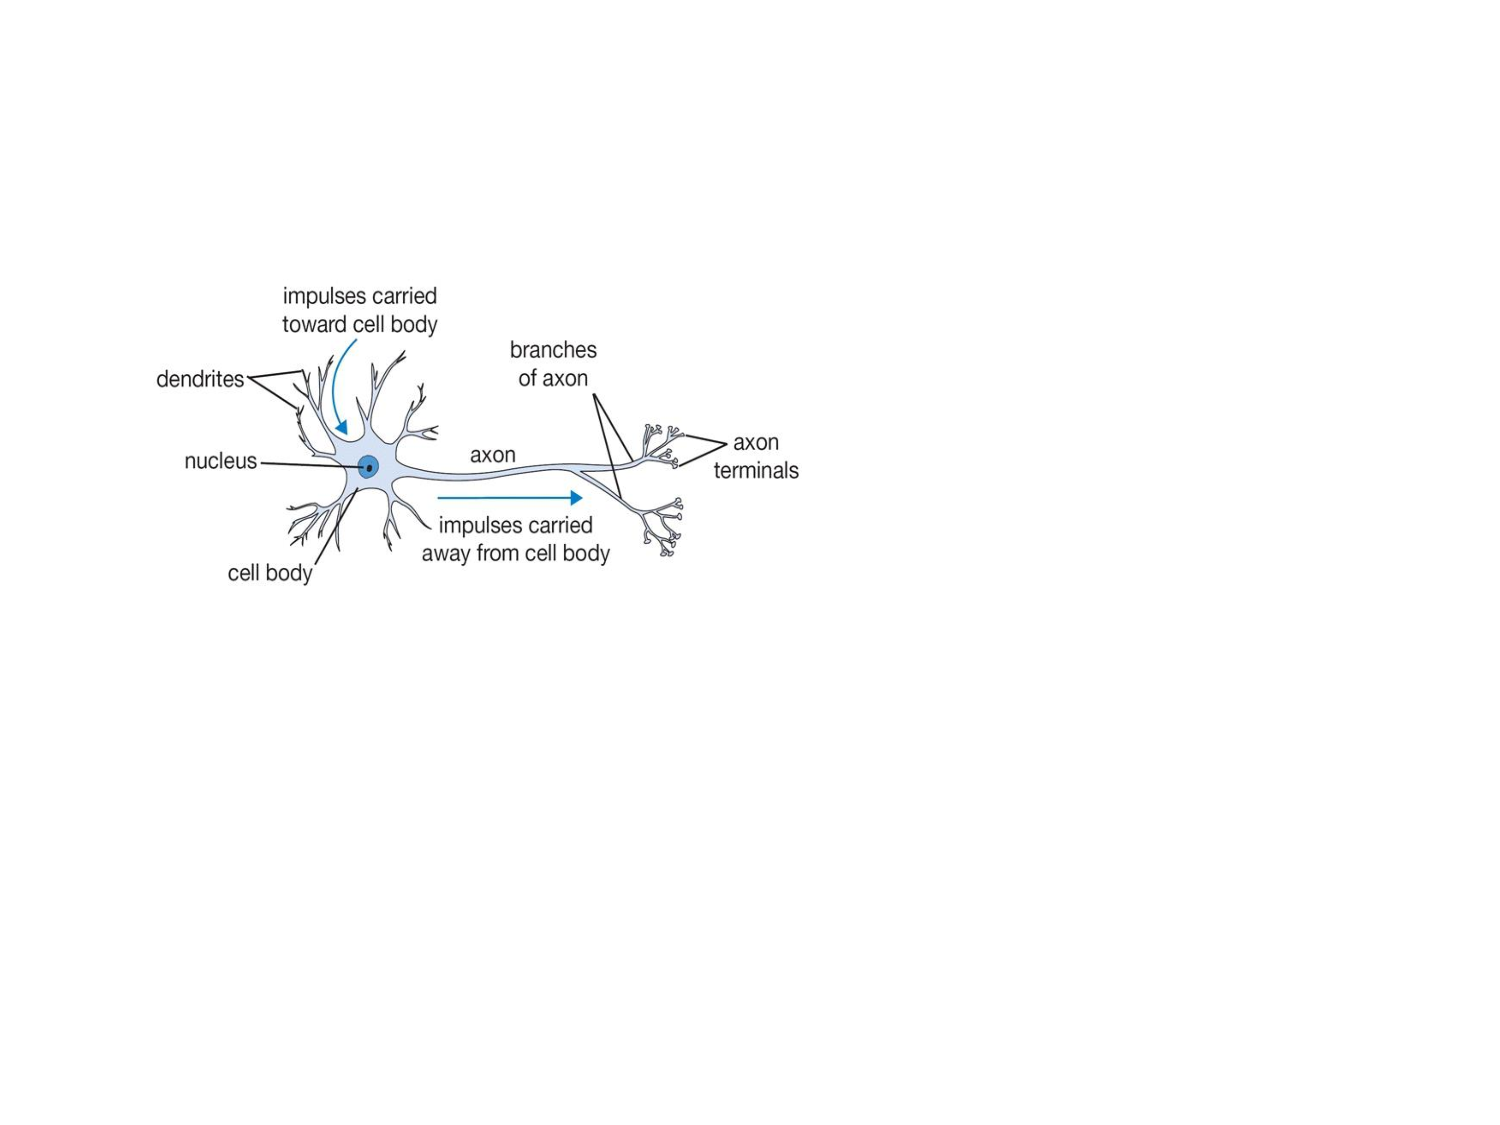
\includegraphics[width=\textwidth]{Biological_neuron}
\onslide<3-5> % Slides 3-5
  \begin{enumerate}
  \item Assign initial weights and random bias.
  \item Scale inputs by multiplying with a weight.
  \\
  \structure{Learning:} Weights are adjusted.
  \item Sum weighted inputs and add offset (bias).
  \\
  \structure{Learning:} Bias is adjusted.
  \item Feed result to an activation function, e.g. a Heaviside step function.
  \end{enumerate}
  \visible<4-5>{
  \alt<4>{Lot of information for very little output (0 or 1). \alert{Can such a model ever be useful on its own?}}%
             {\alert{Such a model can learn a binary (linear) classifier!}}
  }
\end{overprint}
\end{column}
\begin{column}{0.46\textwidth} %% Column 2
\begin{overprint}
\onslide<2-4> % Slides 2-4
\centering
  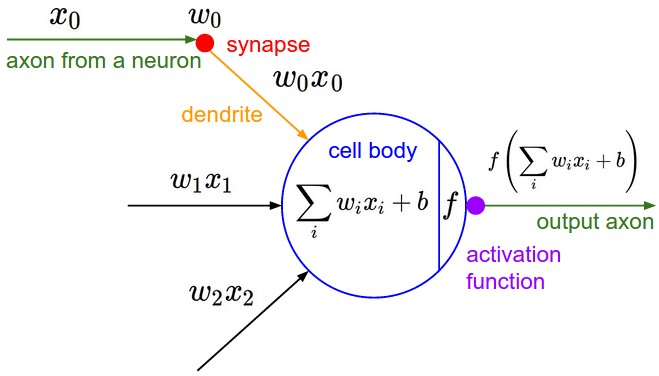
\includegraphics[width=\textwidth]{Artificial_neuron}
%\begin{tikzpicture}[scale=0.75, every node/.style={scale=0.75}]
%  \node[functions] (center) {};
%  \node[below of=center,font=\scriptsize,text width=4em] {Activation function};
%  \draw[thick] (0.5em,0.5em) -- (0,0.5em) -- (0,-0.5em) -- (-0.5em,-0.5em);
%  \draw (0em,0.75em) -- (0em,-0.75em);
%  \draw (0.75em,0em) -- (-0.75em,0em);
%  \node[right of=center] (right) {};
%      \path[draw,->] (center) -- (right);
%  \node[functions,left=3em of center] (left) {$\sum$};
%      \path[draw,->] (left) -- (center);
%  \node[weights,left=3em of left] (2) {$w_3$} -- (2) node[input,left=1.5em of 2] (l2) {$x_3$};
%      \path[draw,->] (l2) -- (2);
%      \path[draw,->] (2) -- (left);
%  \node[below of=2] (dots) {$\vdots$} -- (dots) node[left=2.5em of dots] (ldots) {$\vdots$};
%  \node[weights,below of=dots] (n) {$w_n$} -- (n) node[input,left=1.5em of n] (ln) {$x_n$};
%      \path[draw,->] (ln) -- (n);
%      \path[draw,->] (n) -- (left);
%  \node[weights,above of=2] (1) {$w_2$} -- (1) node[input,left=1.5em of 1] (l1) {$x_2$};
%      \path[draw,->] (l1) -- (1);
%      \path[draw,->] (1) -- (left);
%  \node[weights,above of=1] (0) {$w_1$} -- (0) node[input,left=1.5em of 0] (l0) {$x_1$};
%      \path[draw,->] (l0) -- (0);
%      \path[draw,->] (0) -- (left);
%  \node[below of=ln,font=\scriptsize]{Inputs};
%  \node[below of=n,font=\scriptsize]{Weights};
%\end{tikzpicture}
\onslide<5> % Slide 5
  \begin{center}
  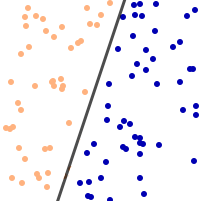
\includegraphics[width=0.4\textwidth]{LinearClassifier}
  \end{center}
  \vskip-0.5\baselineskip
  Binary classifier: Train $\param = (w,b) \in \Real^{2n}$
  \[ \model_{\param}(x) := \begin{cases} 1 & \text{if $\langle w, x\rangle +b > 0$} \\ 0 & \text{ otherwise.} \end{cases} \]
\end{overprint}
\end{column}
\end{columns}
\end{frame}

%\begin{frame}{Network architectures}{Response of single neuron}
%\begin{center}
%\begin{overprint}
%\onslide<1>
%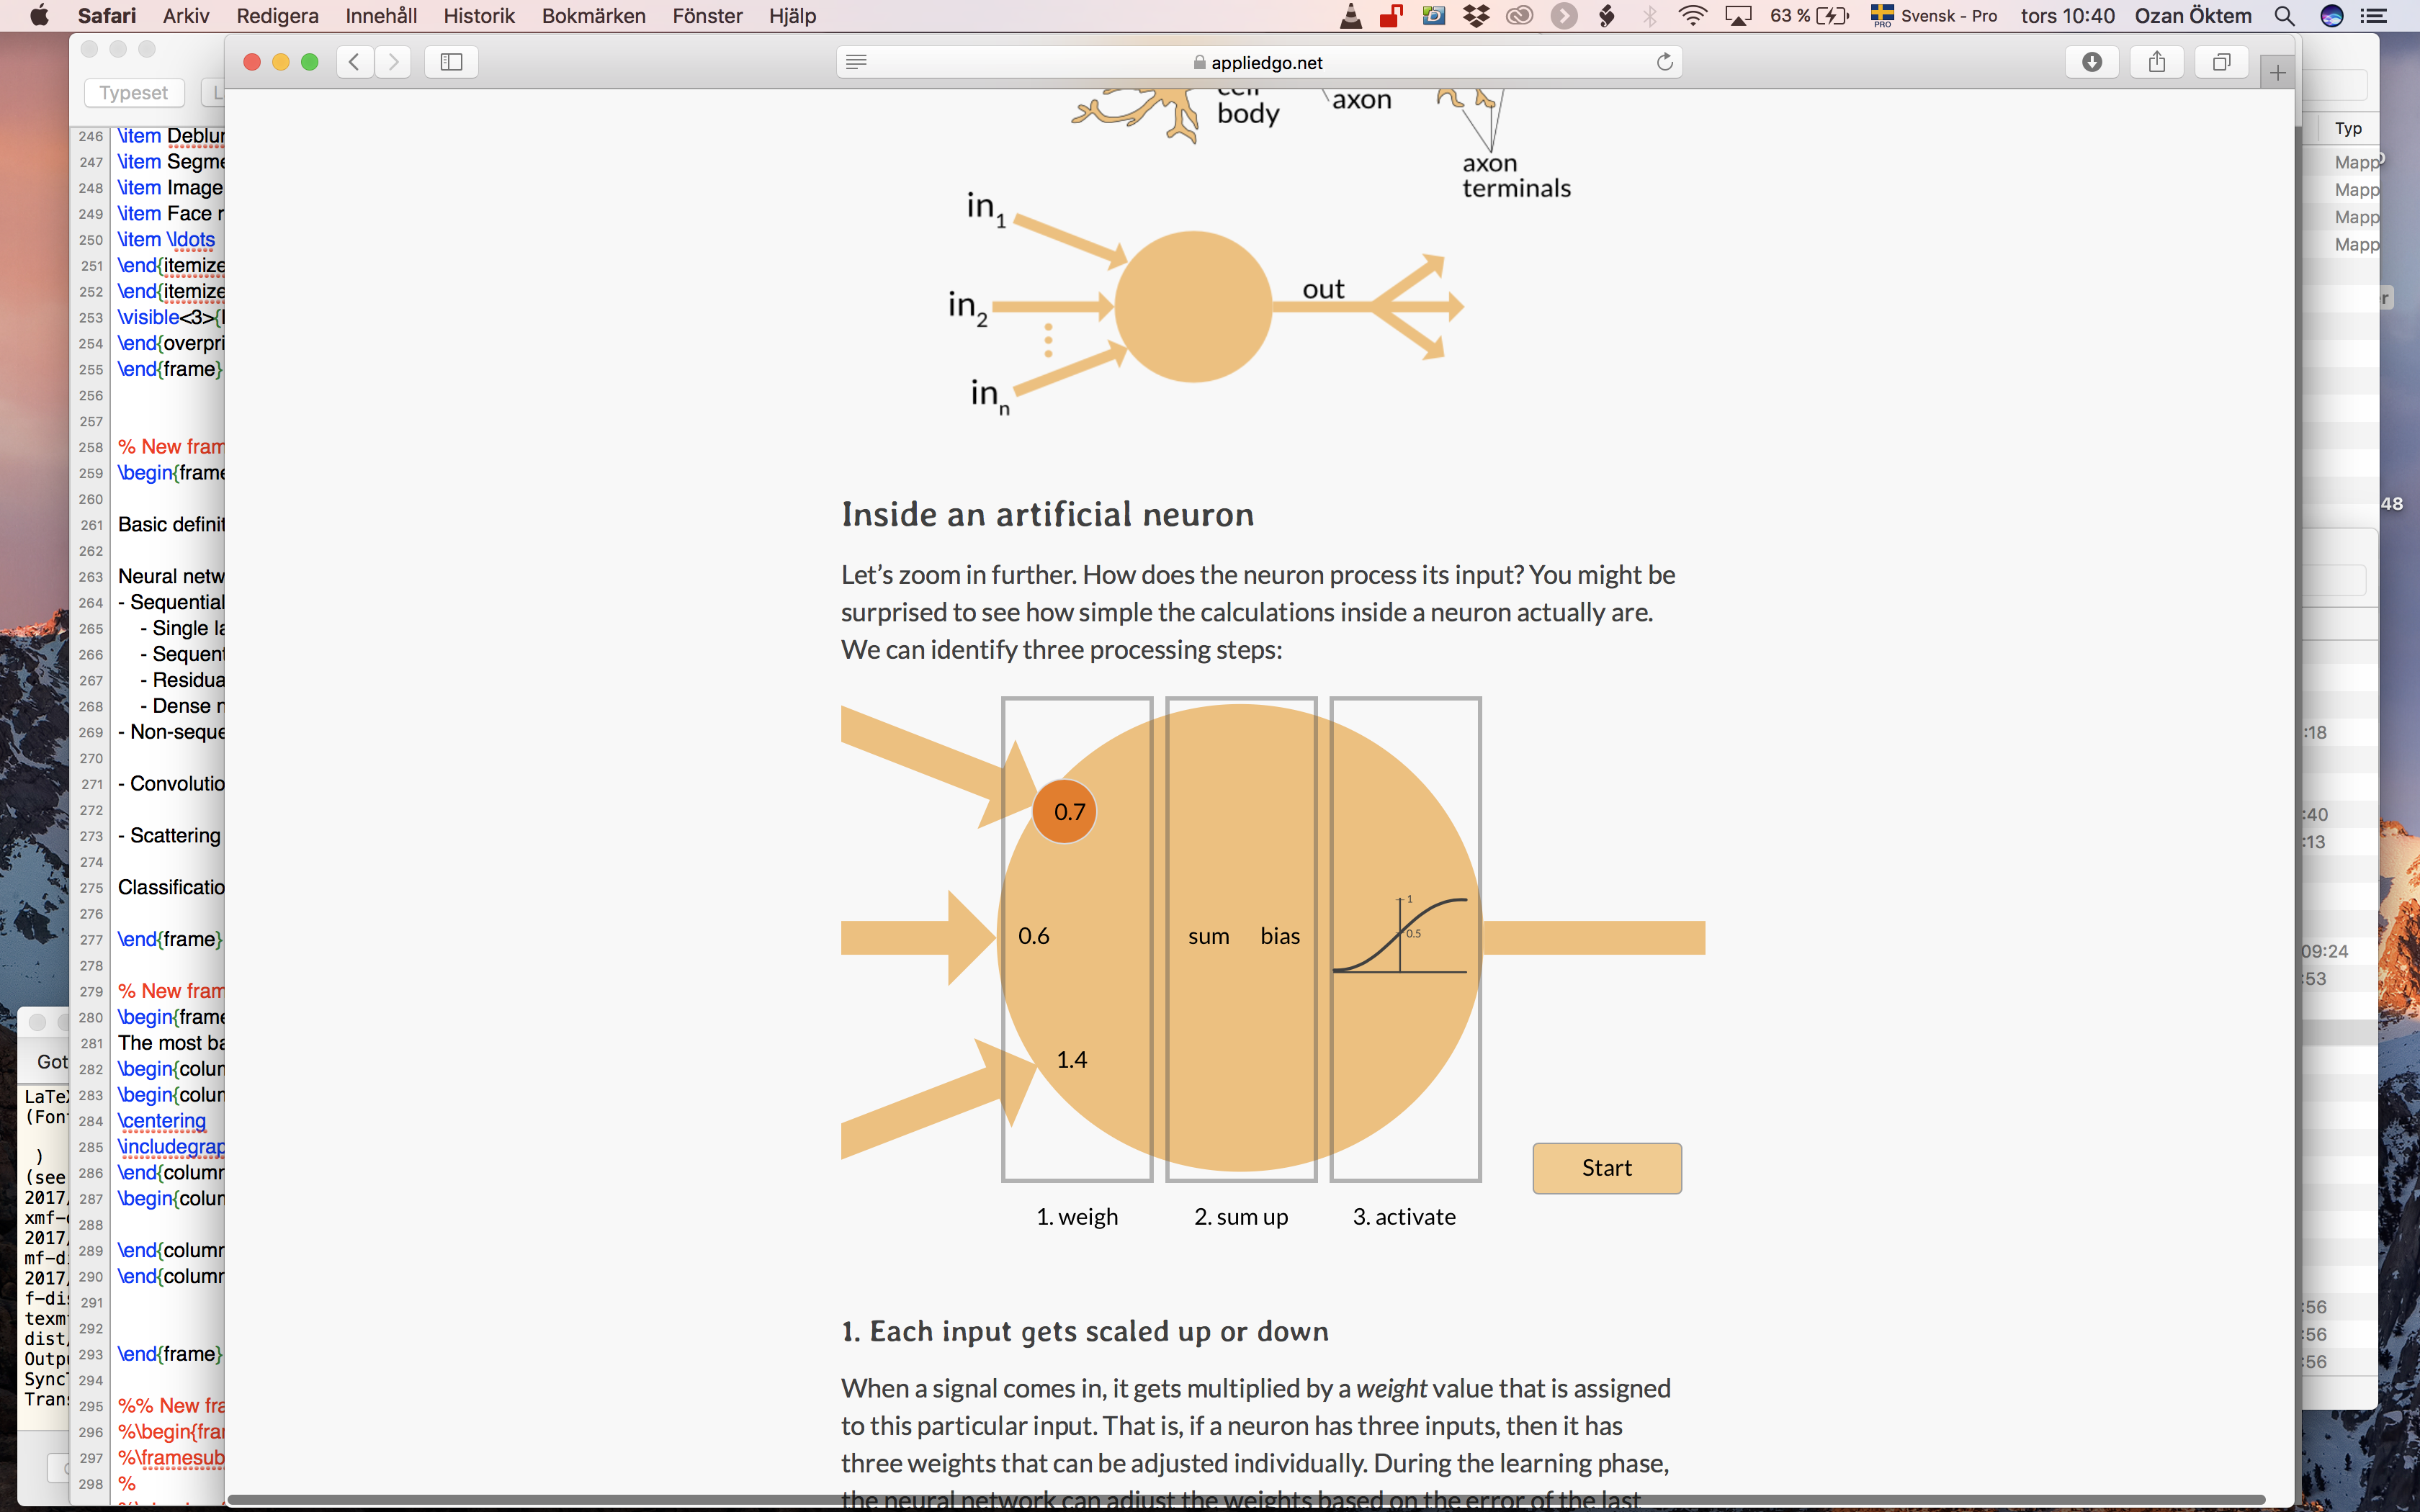
\includegraphics[trim={585 195 495 483},clip,height=0.9\textheight]{step1}
%\onslide<2>
%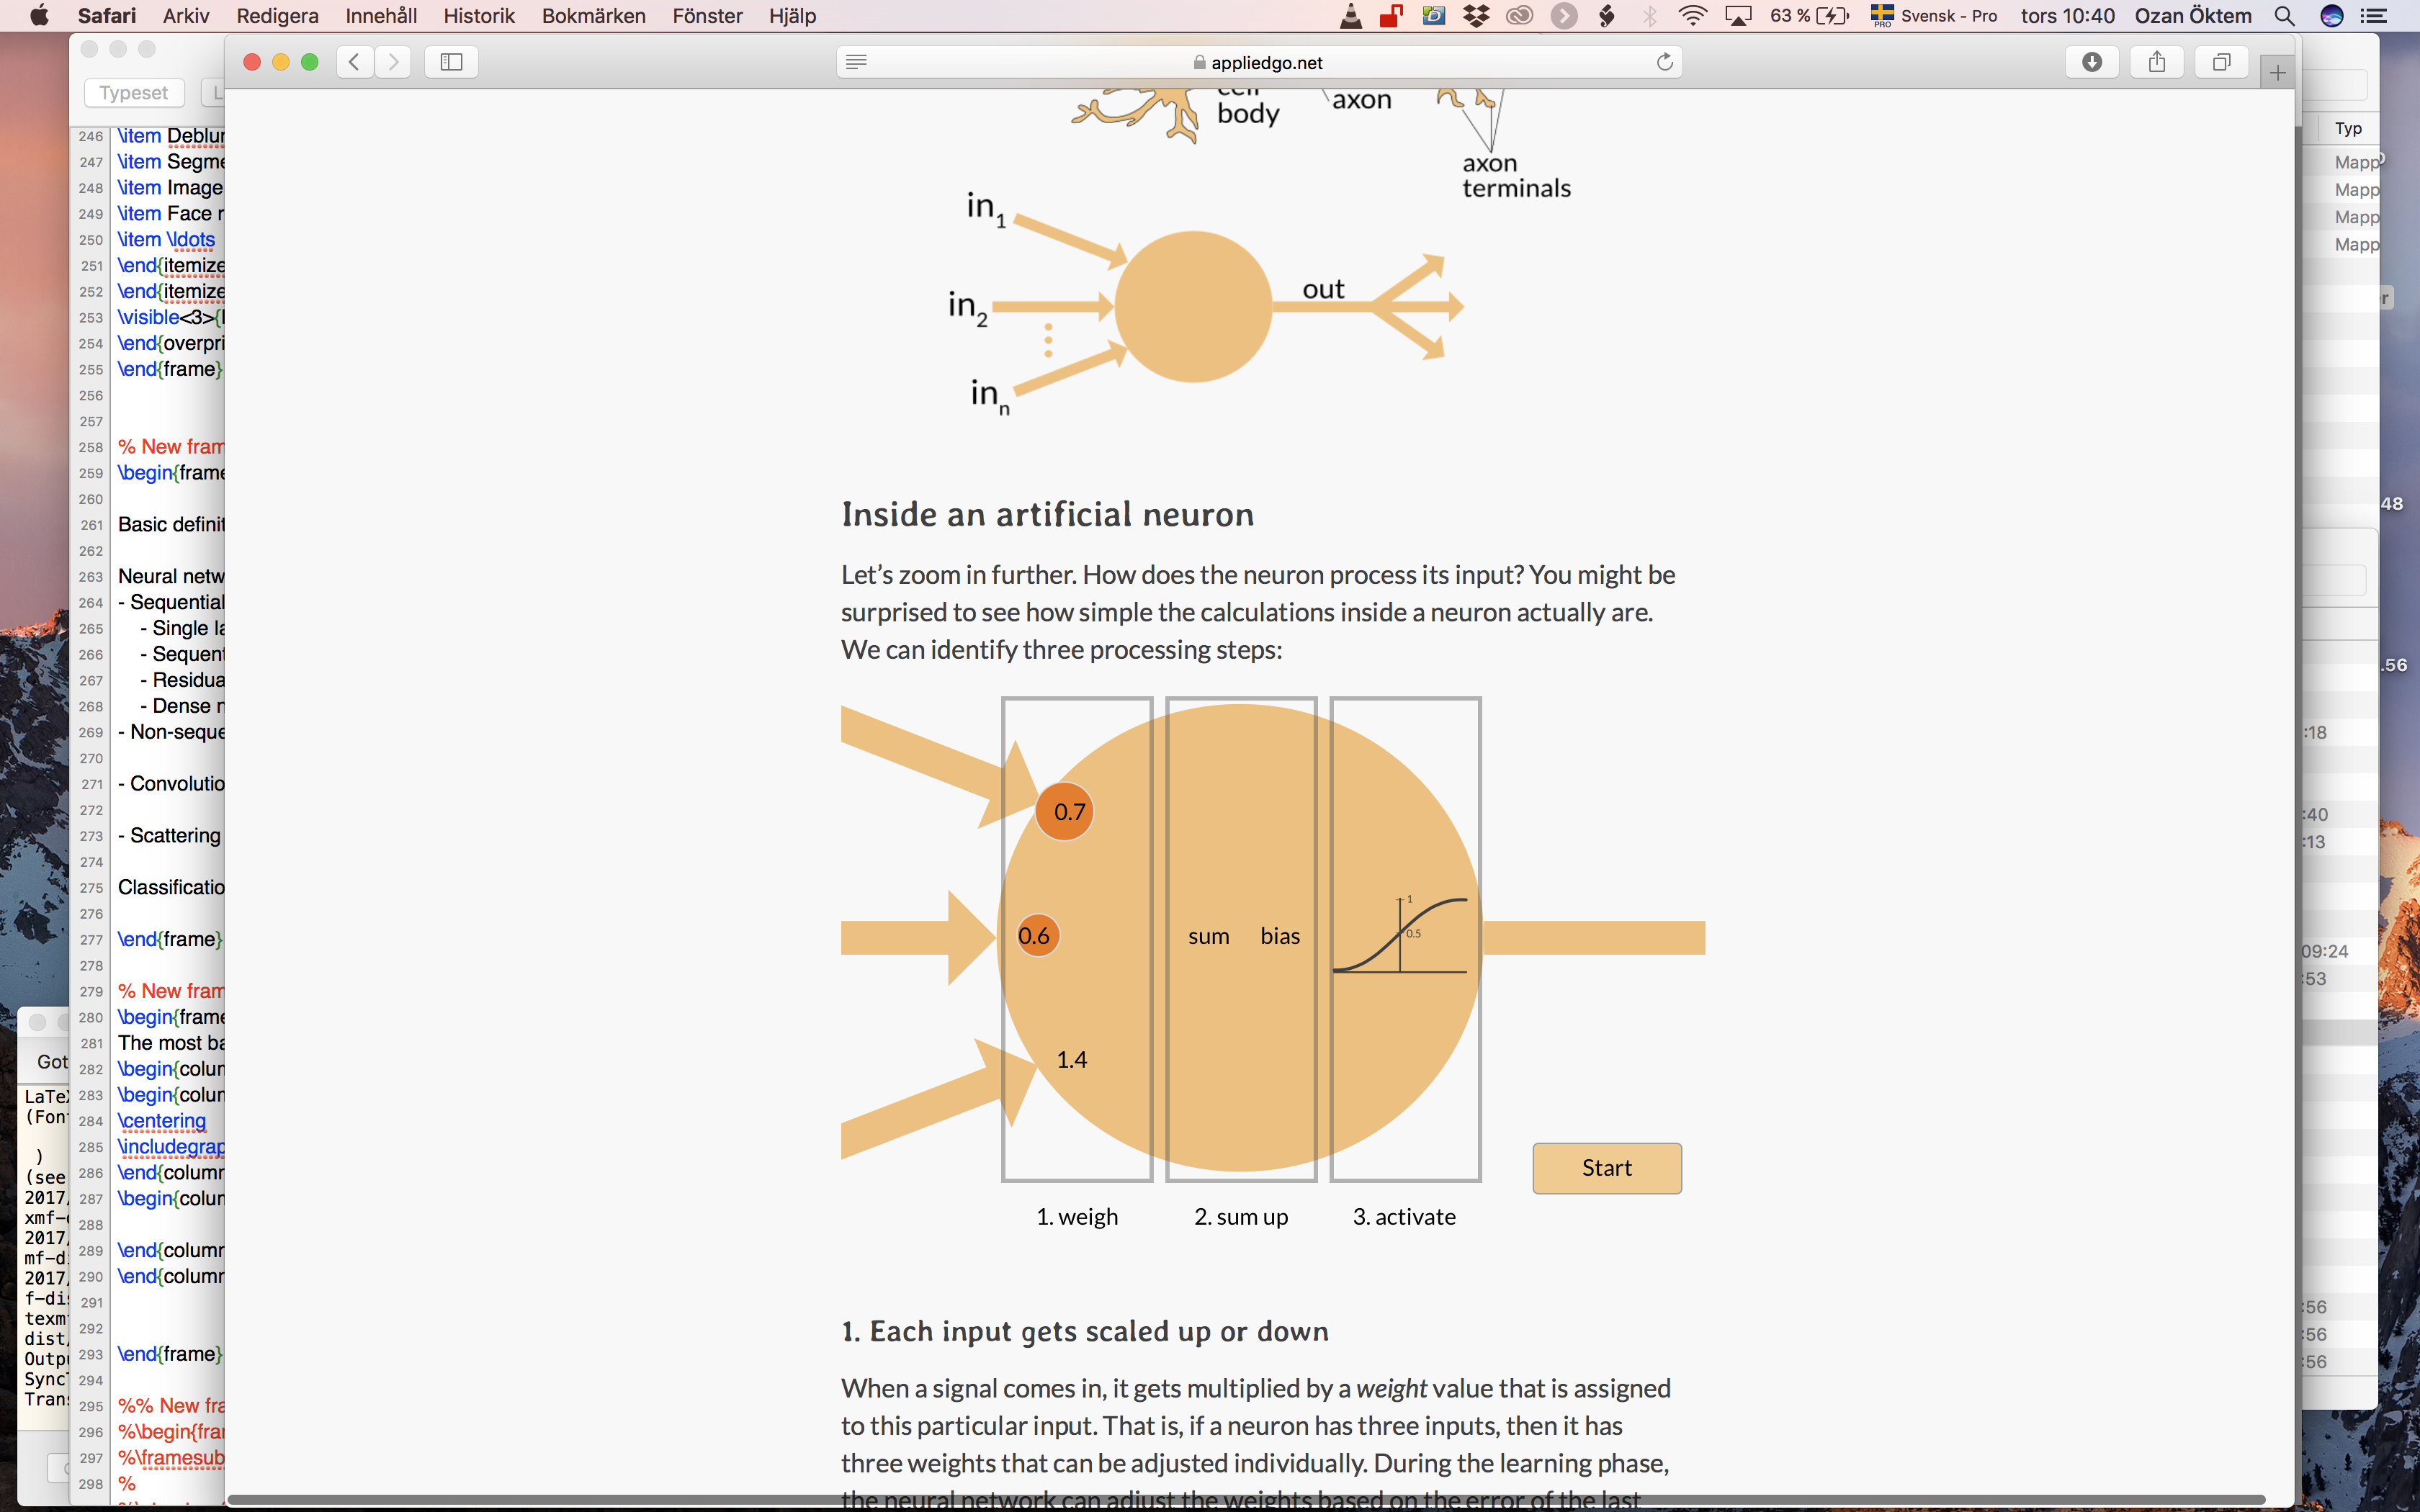
\includegraphics[trim={585 195 495 483},clip,height=0.9\textheight]{step2}
%\onslide<3>
%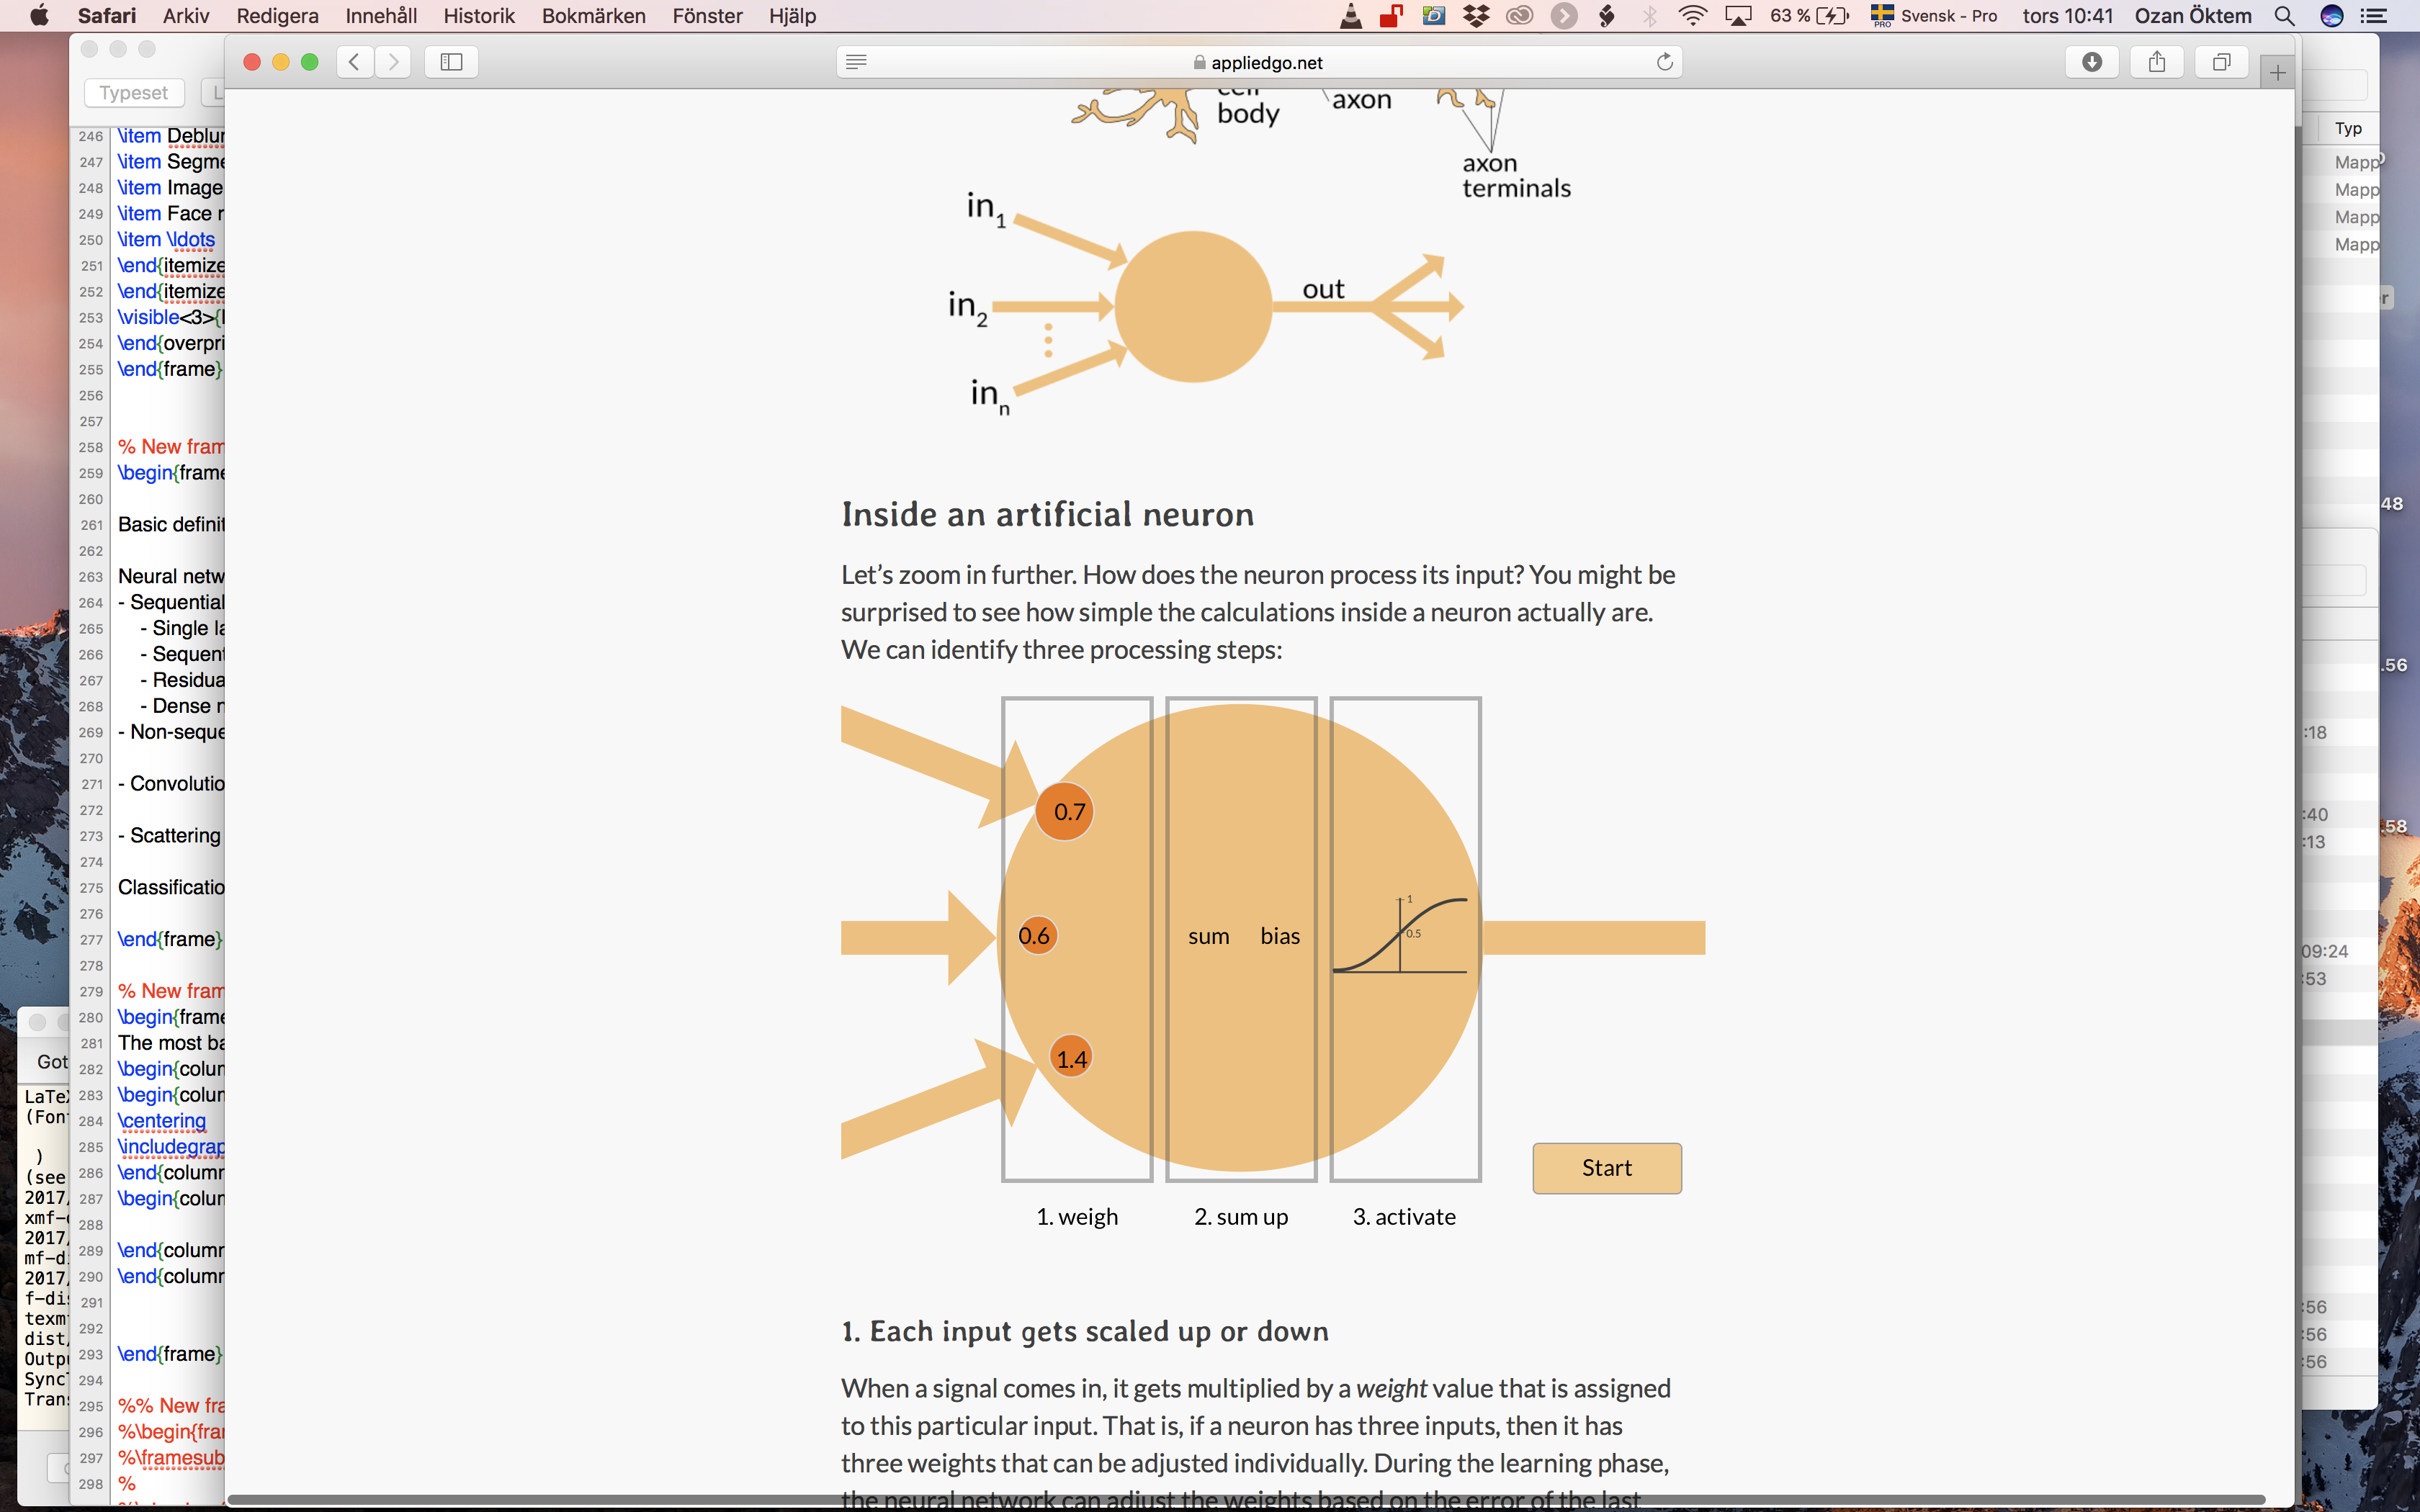
\includegraphics[trim={585 195 495 483},clip,height=0.9\textheight]{step3}
%\onslide<4>
%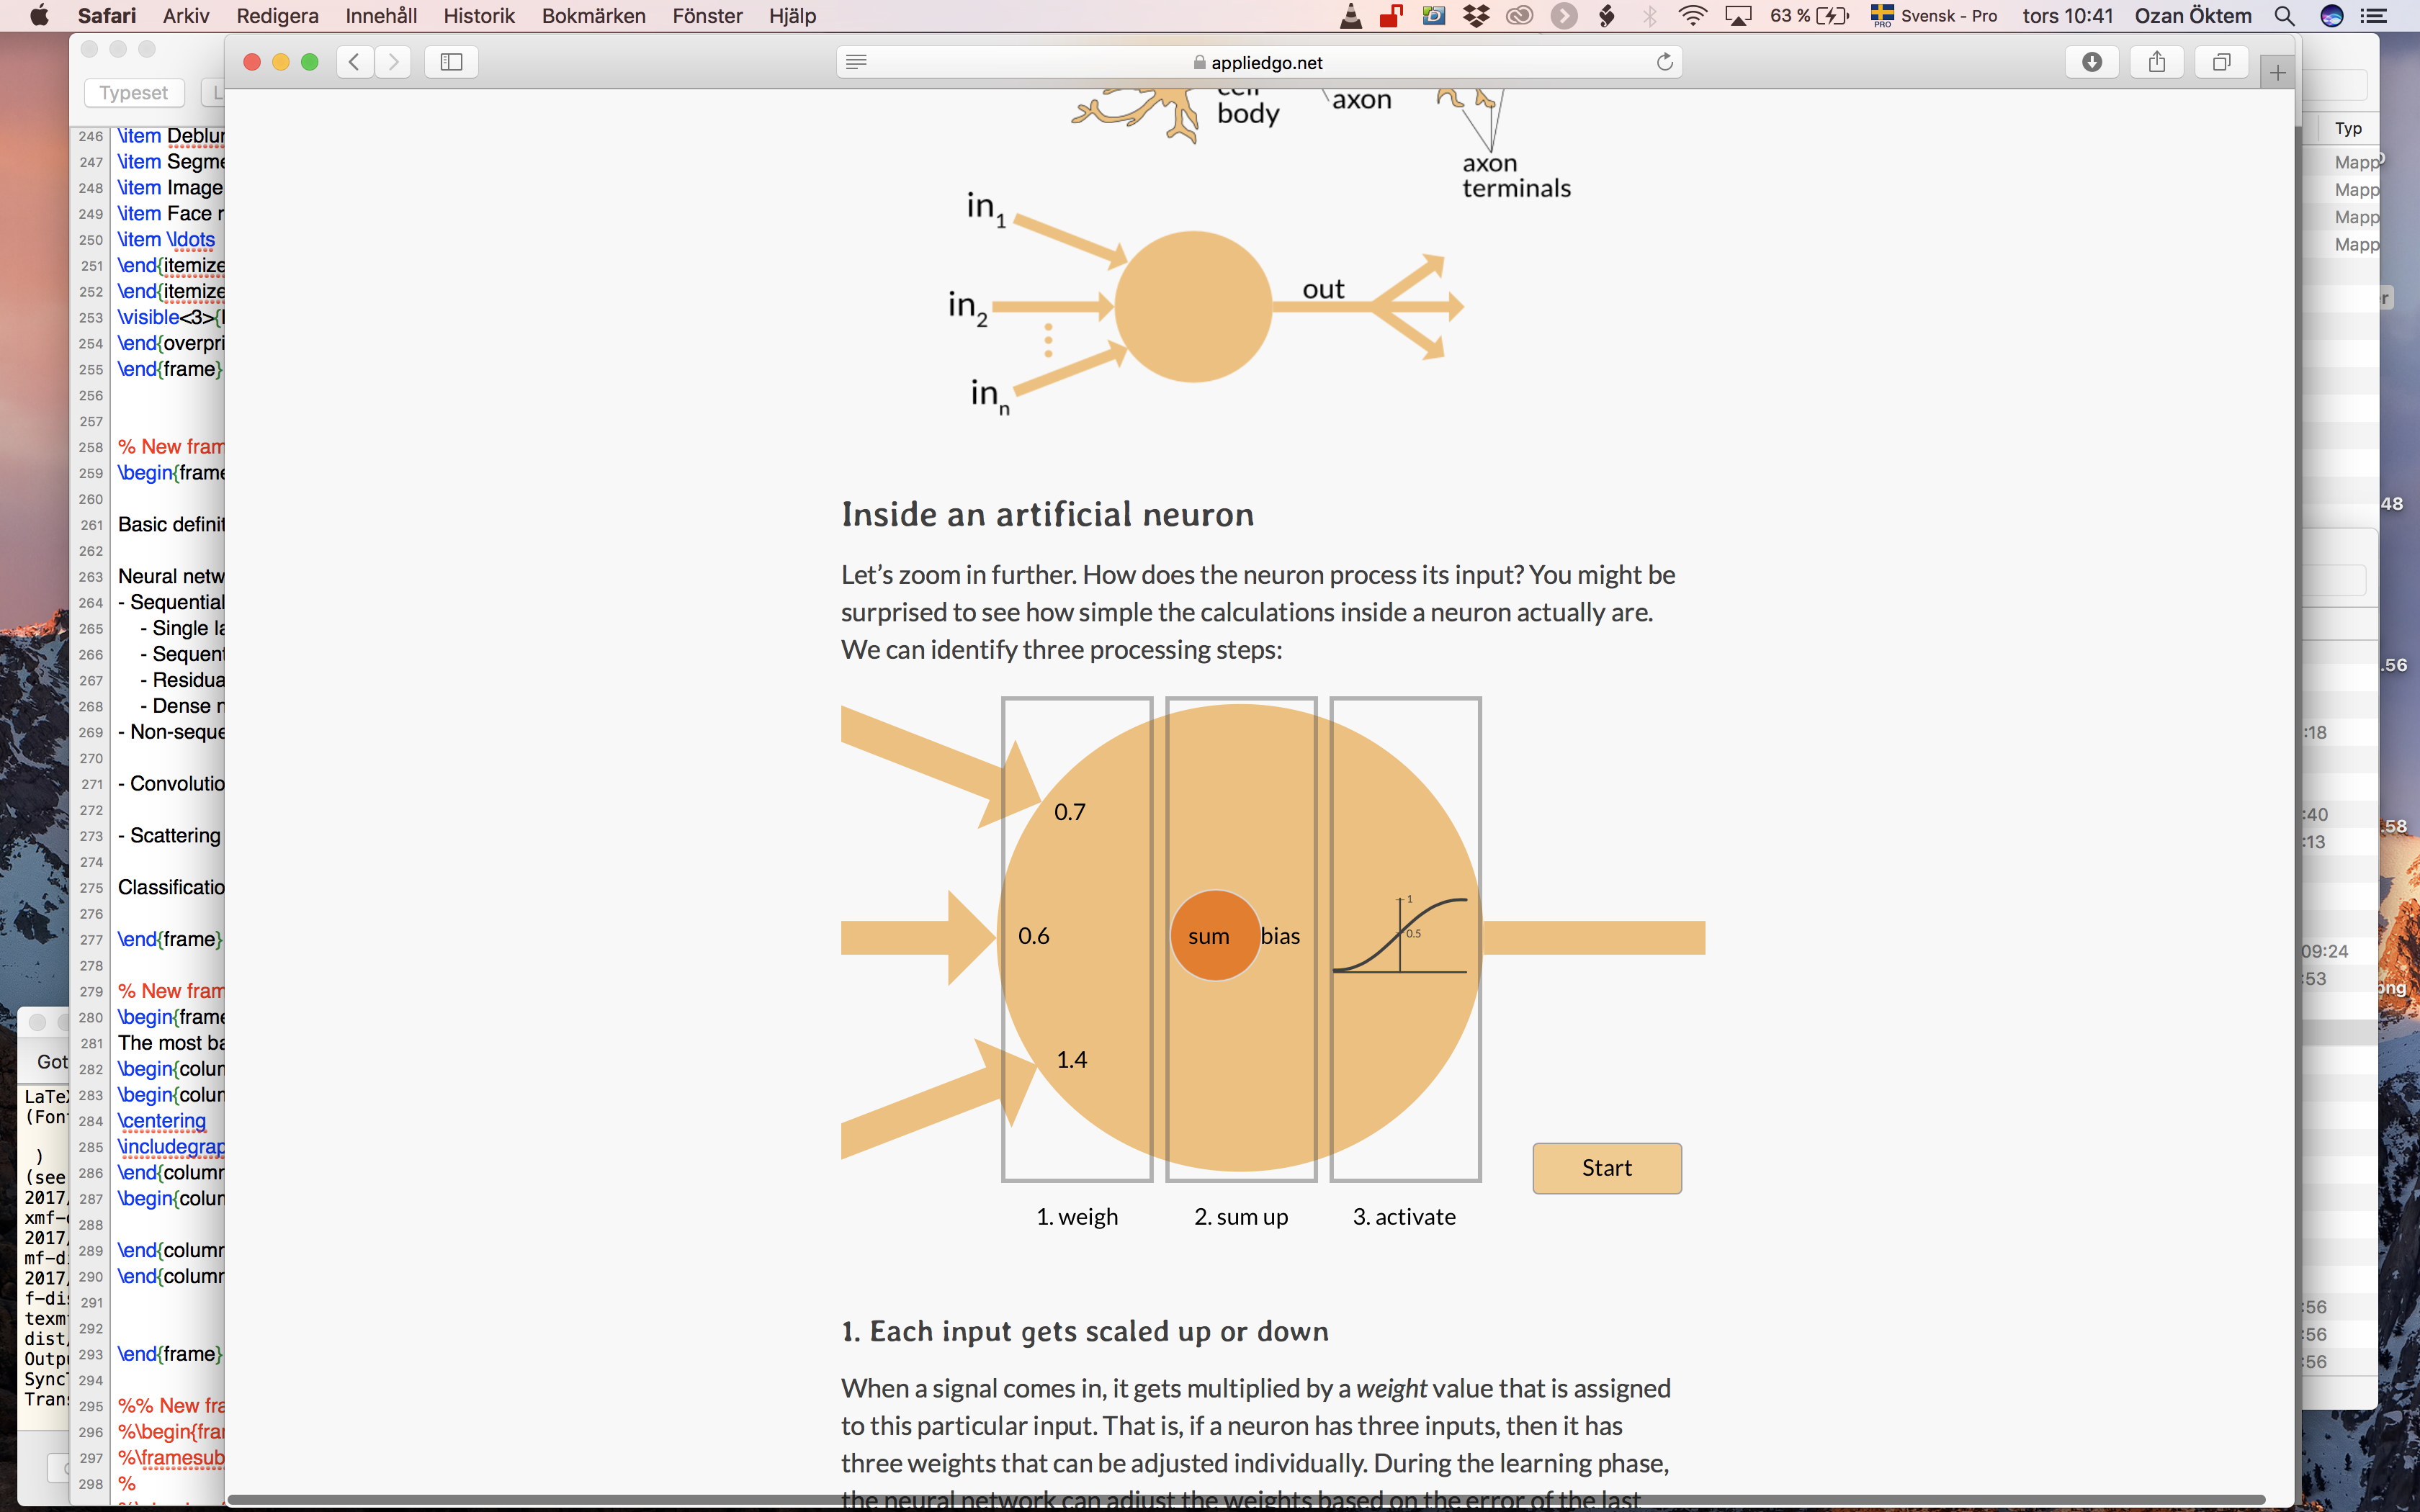
\includegraphics[trim={585 195 495 483},clip,height=0.9\textheight]{step4}
%\onslide<5>
%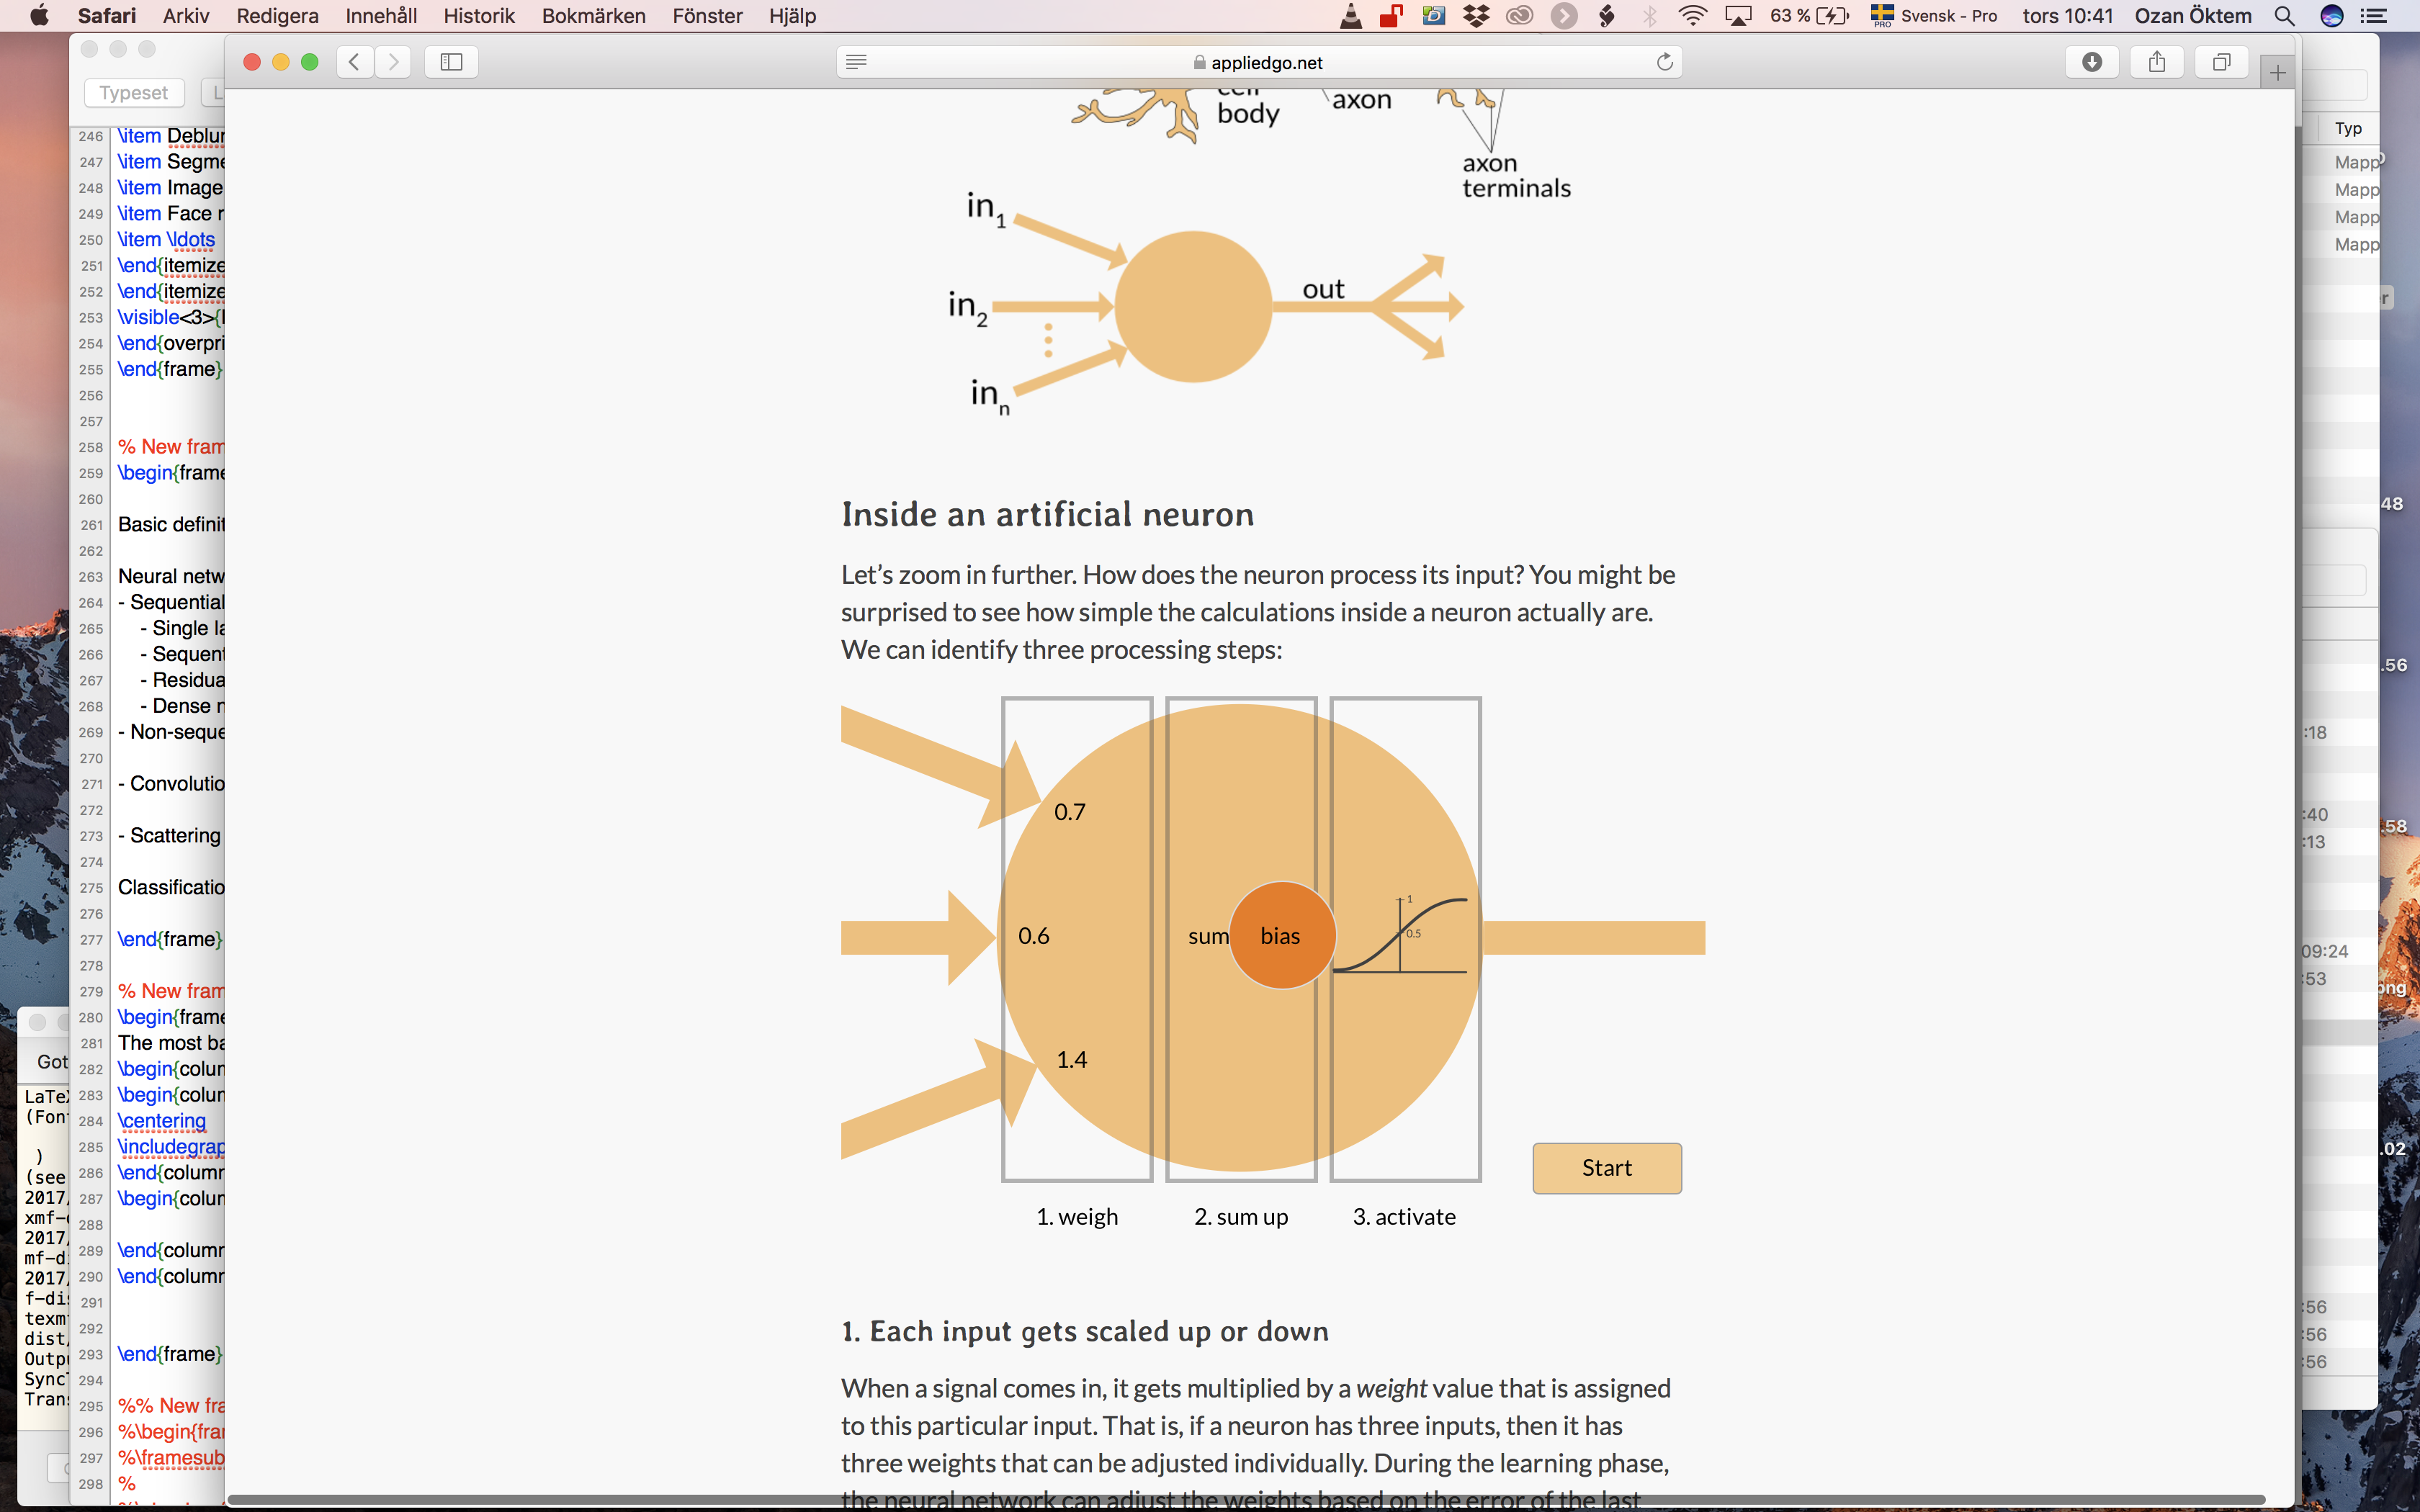
\includegraphics[trim={585 195 495 483},clip,height=0.9\textheight]{step5}
%\onslide<6>
%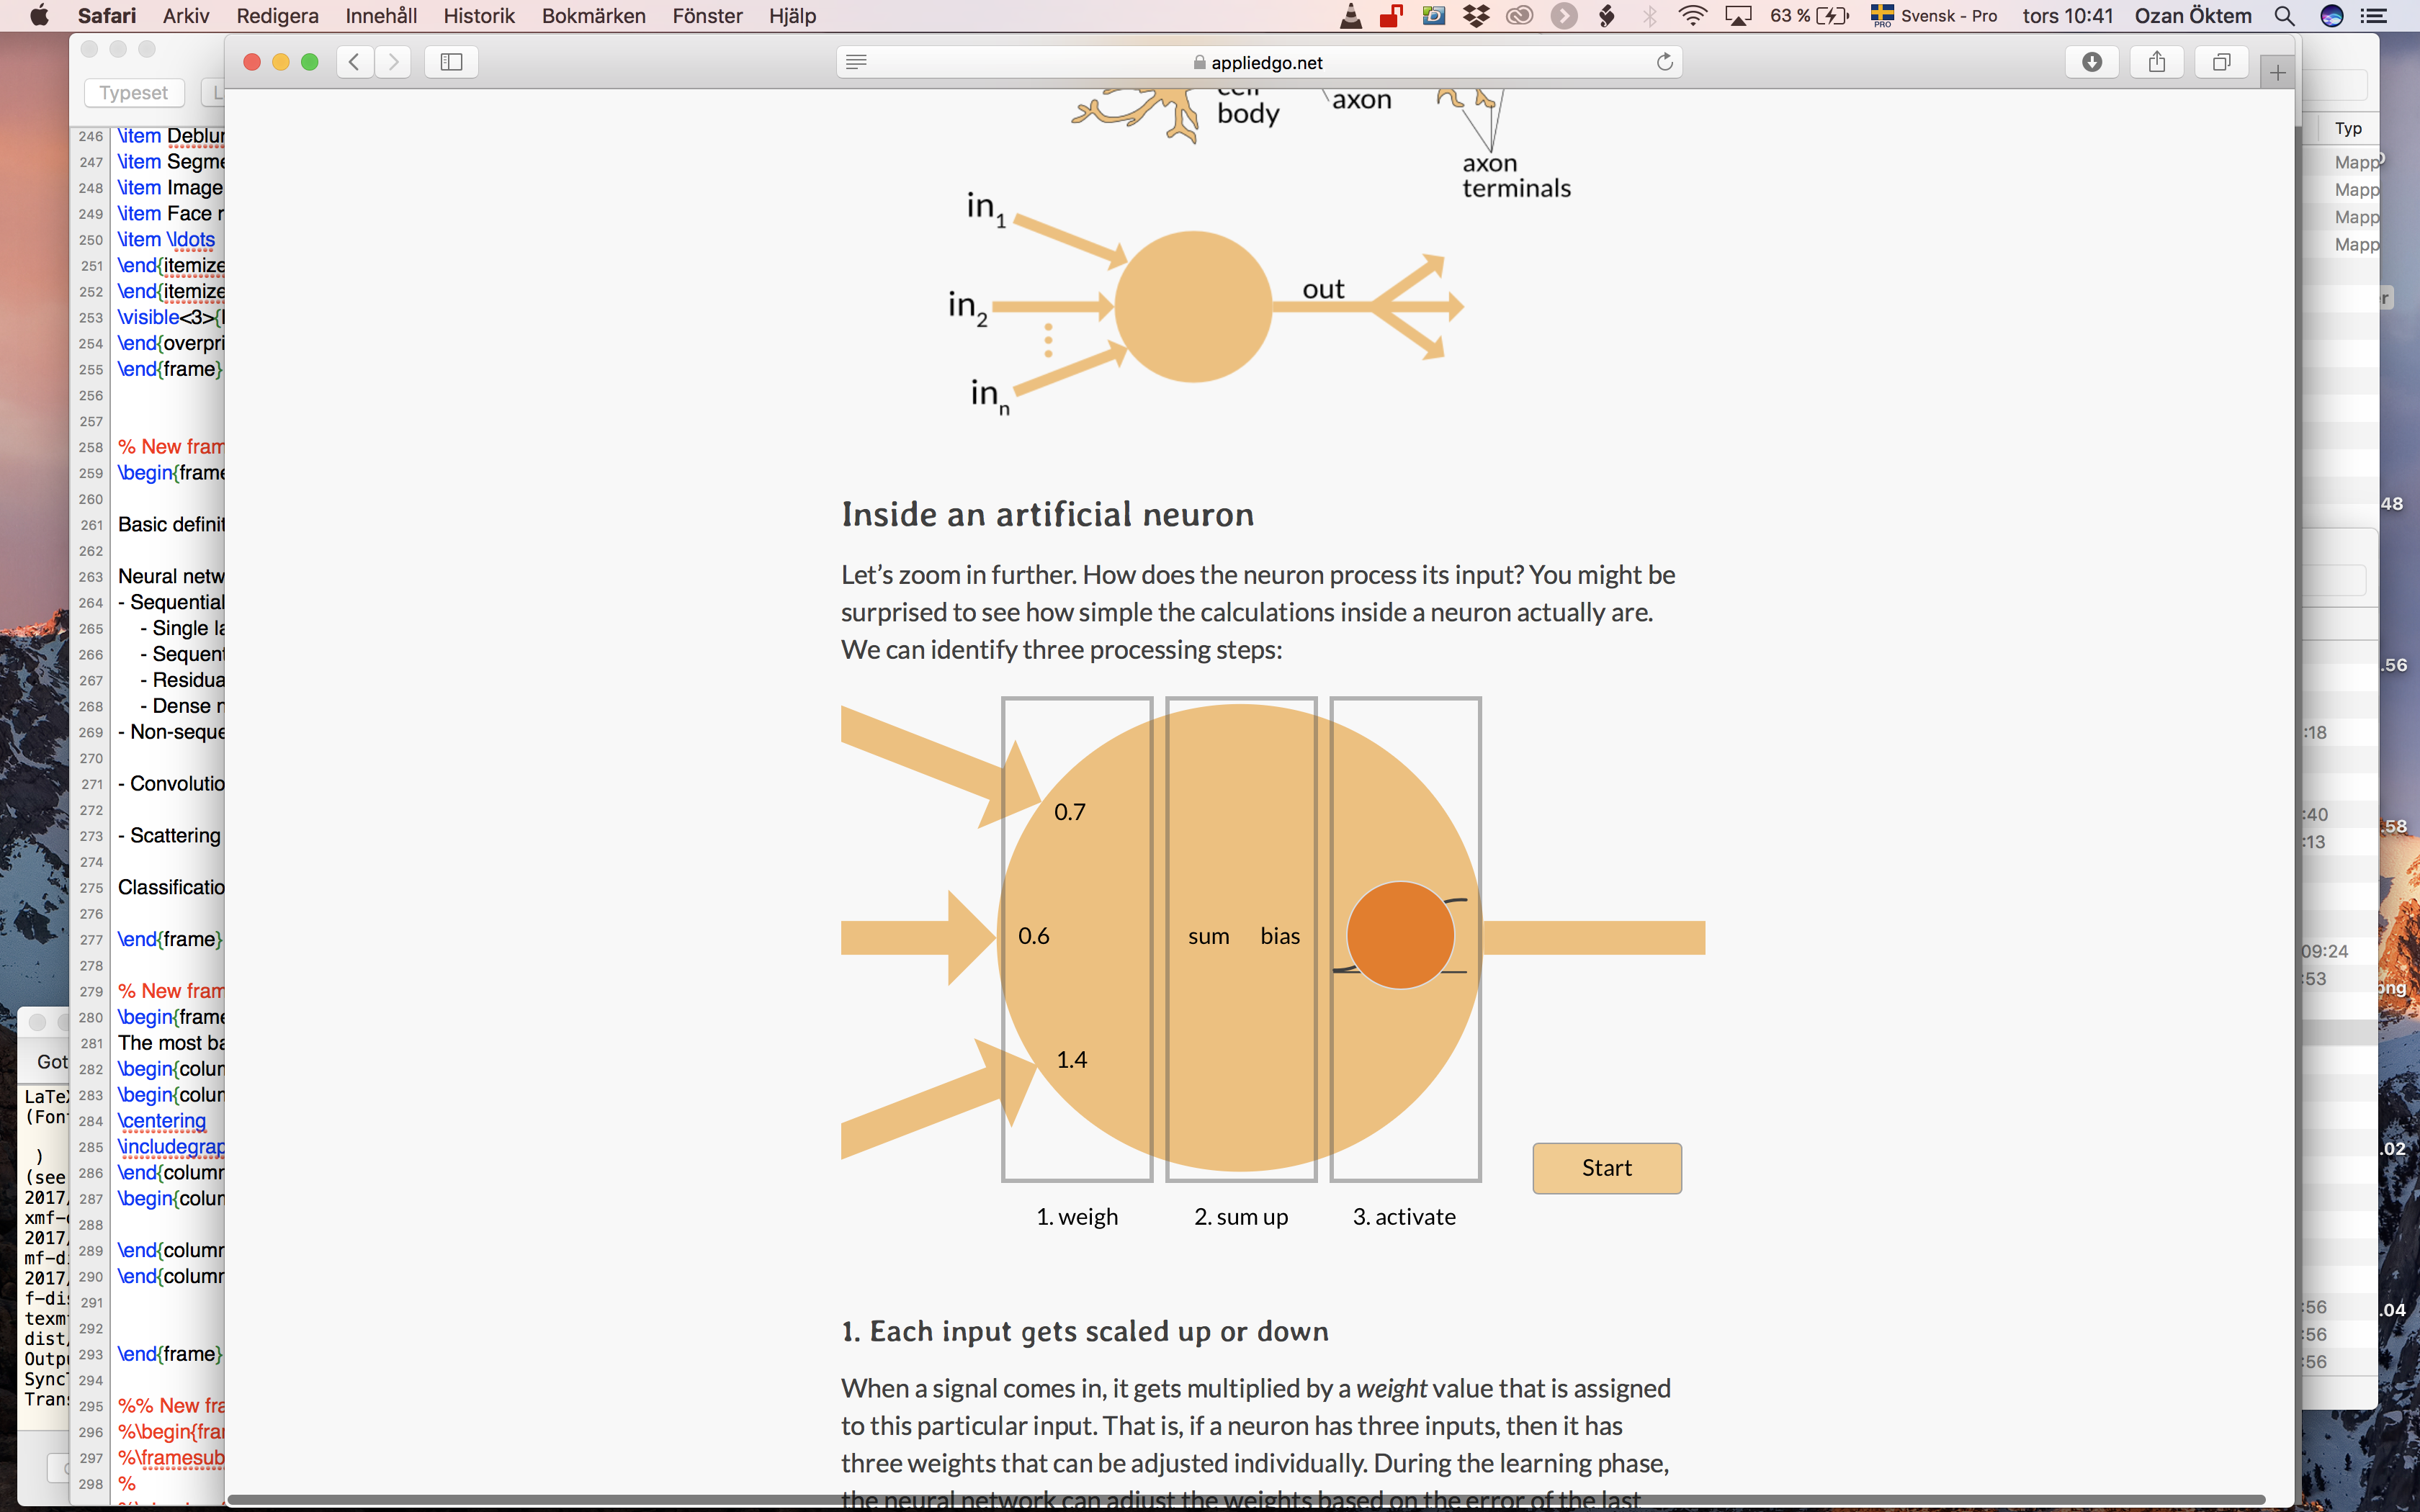
\includegraphics[trim={585 195 495 483},clip,height=0.9\textheight]{step6}
%\onslide<7>
%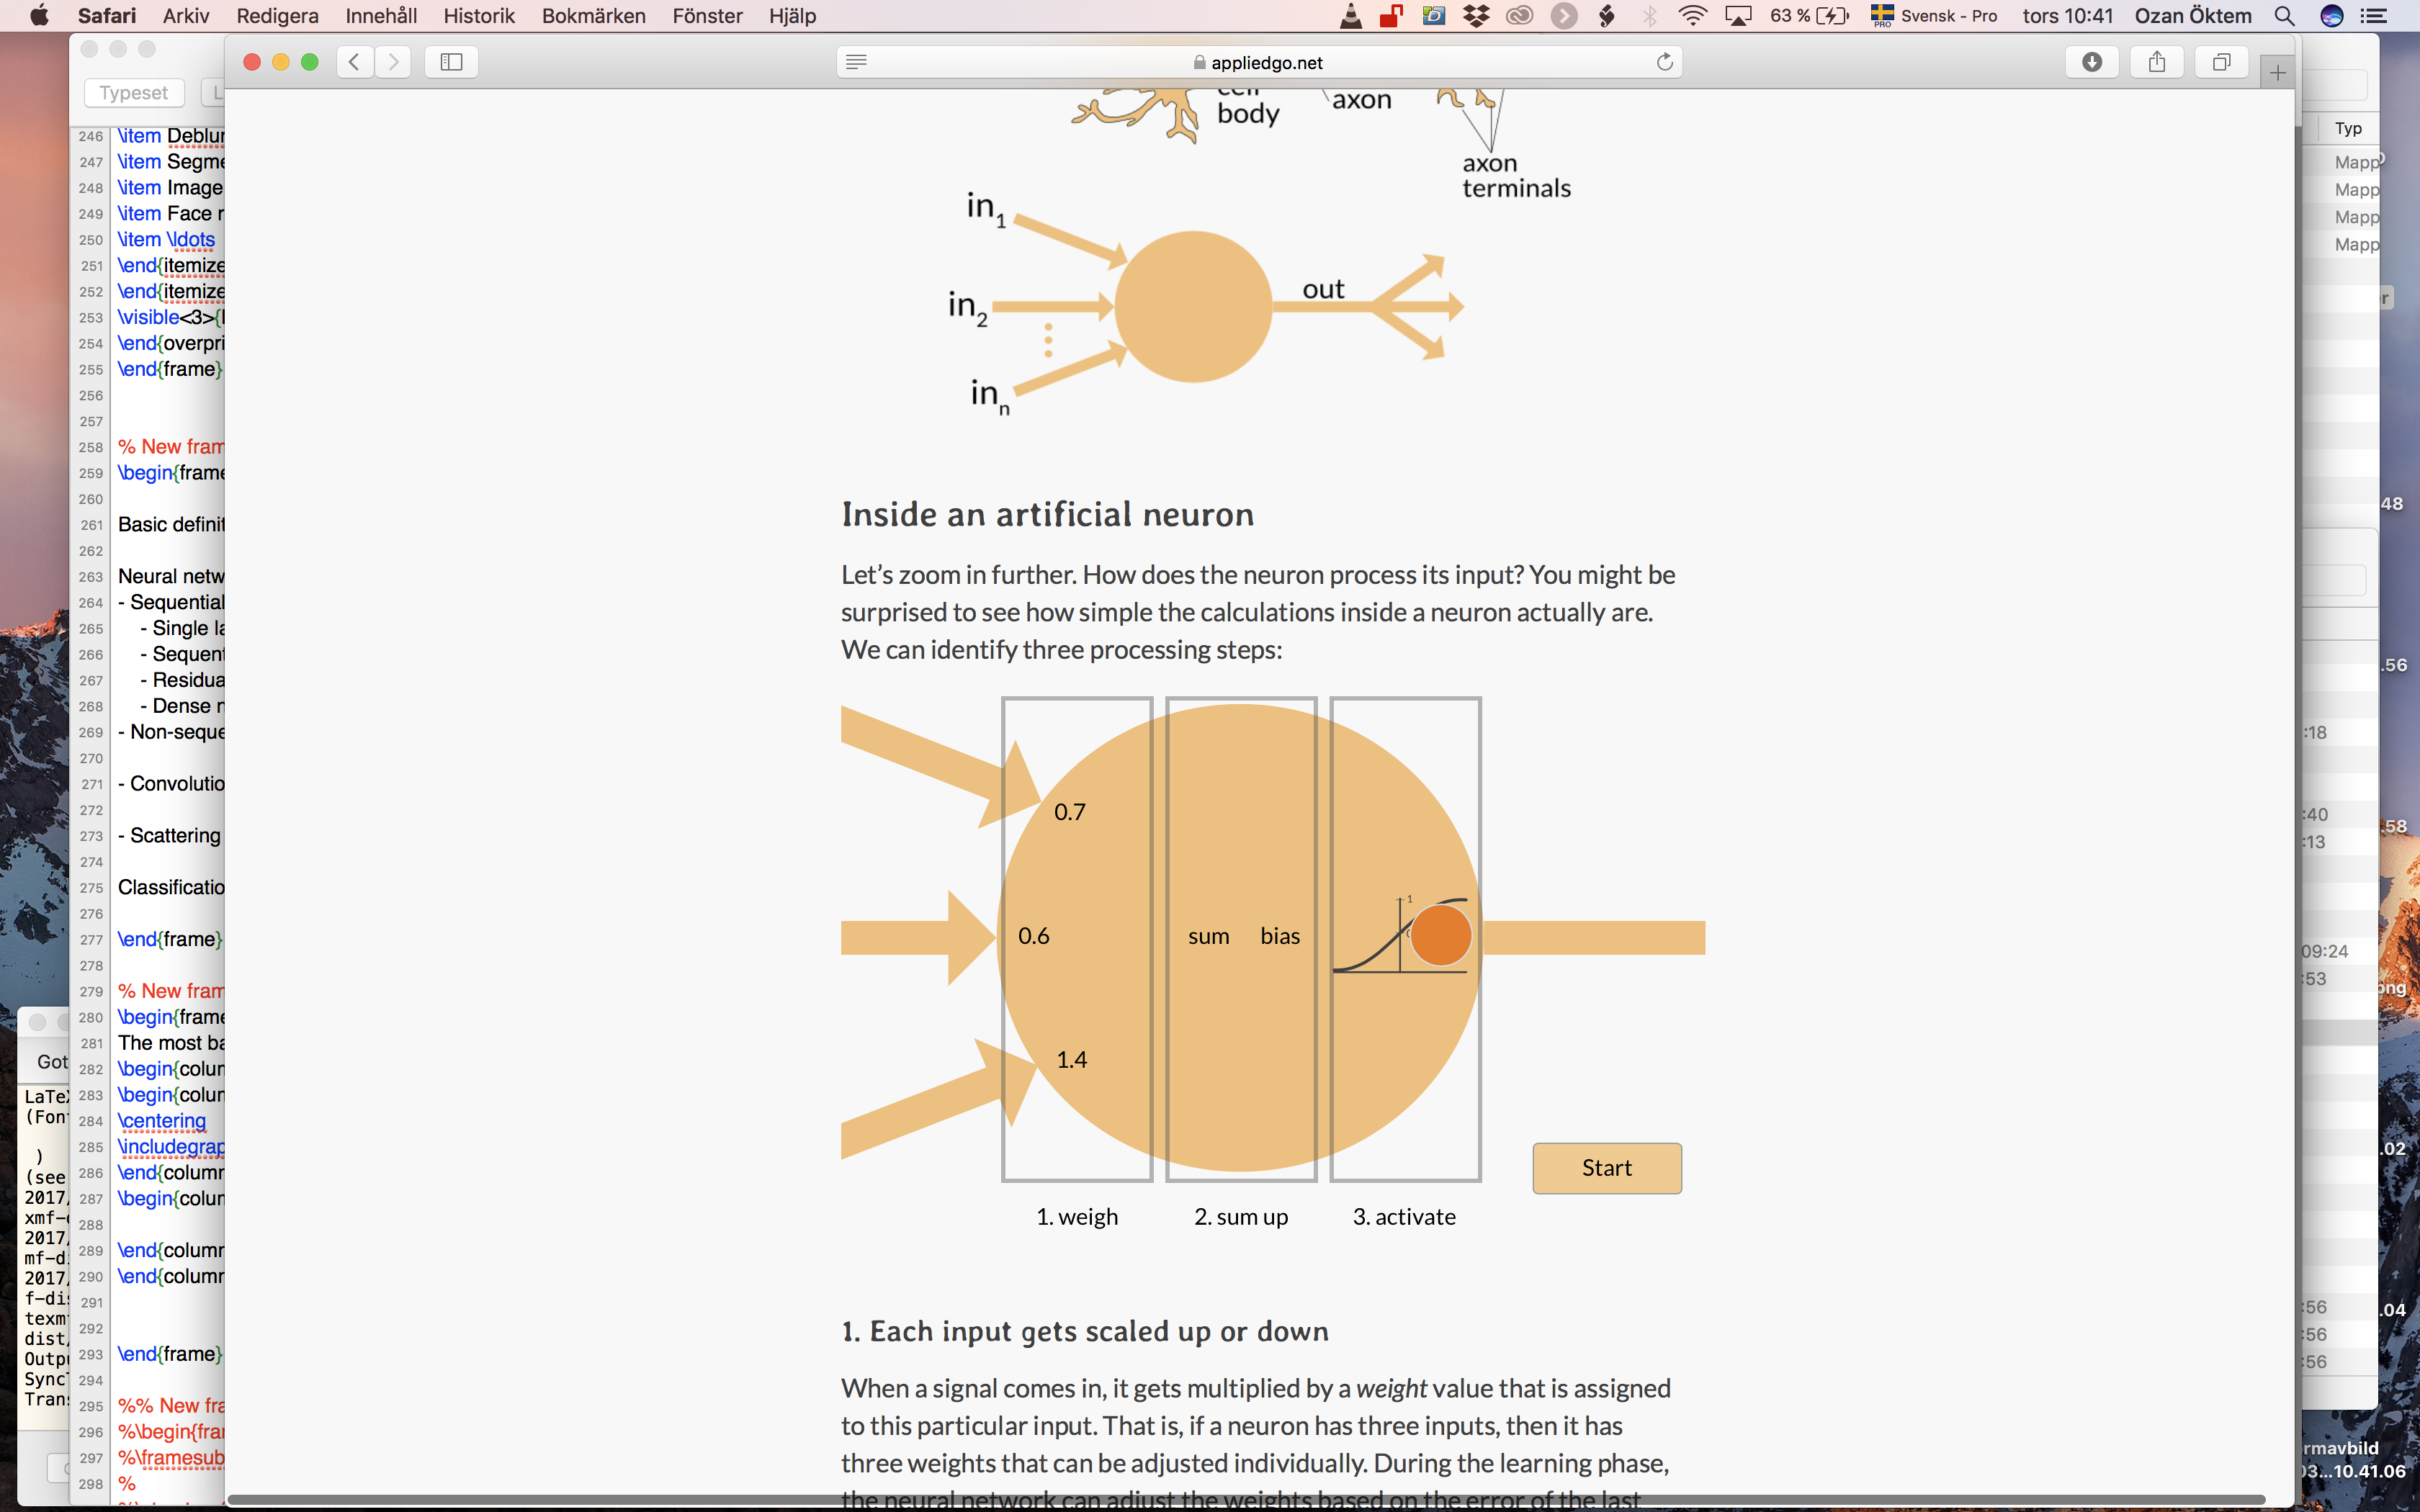
\includegraphics[trim={585 195 495 483},clip,height=0.9\textheight]{step7}
%\onslide<8>
%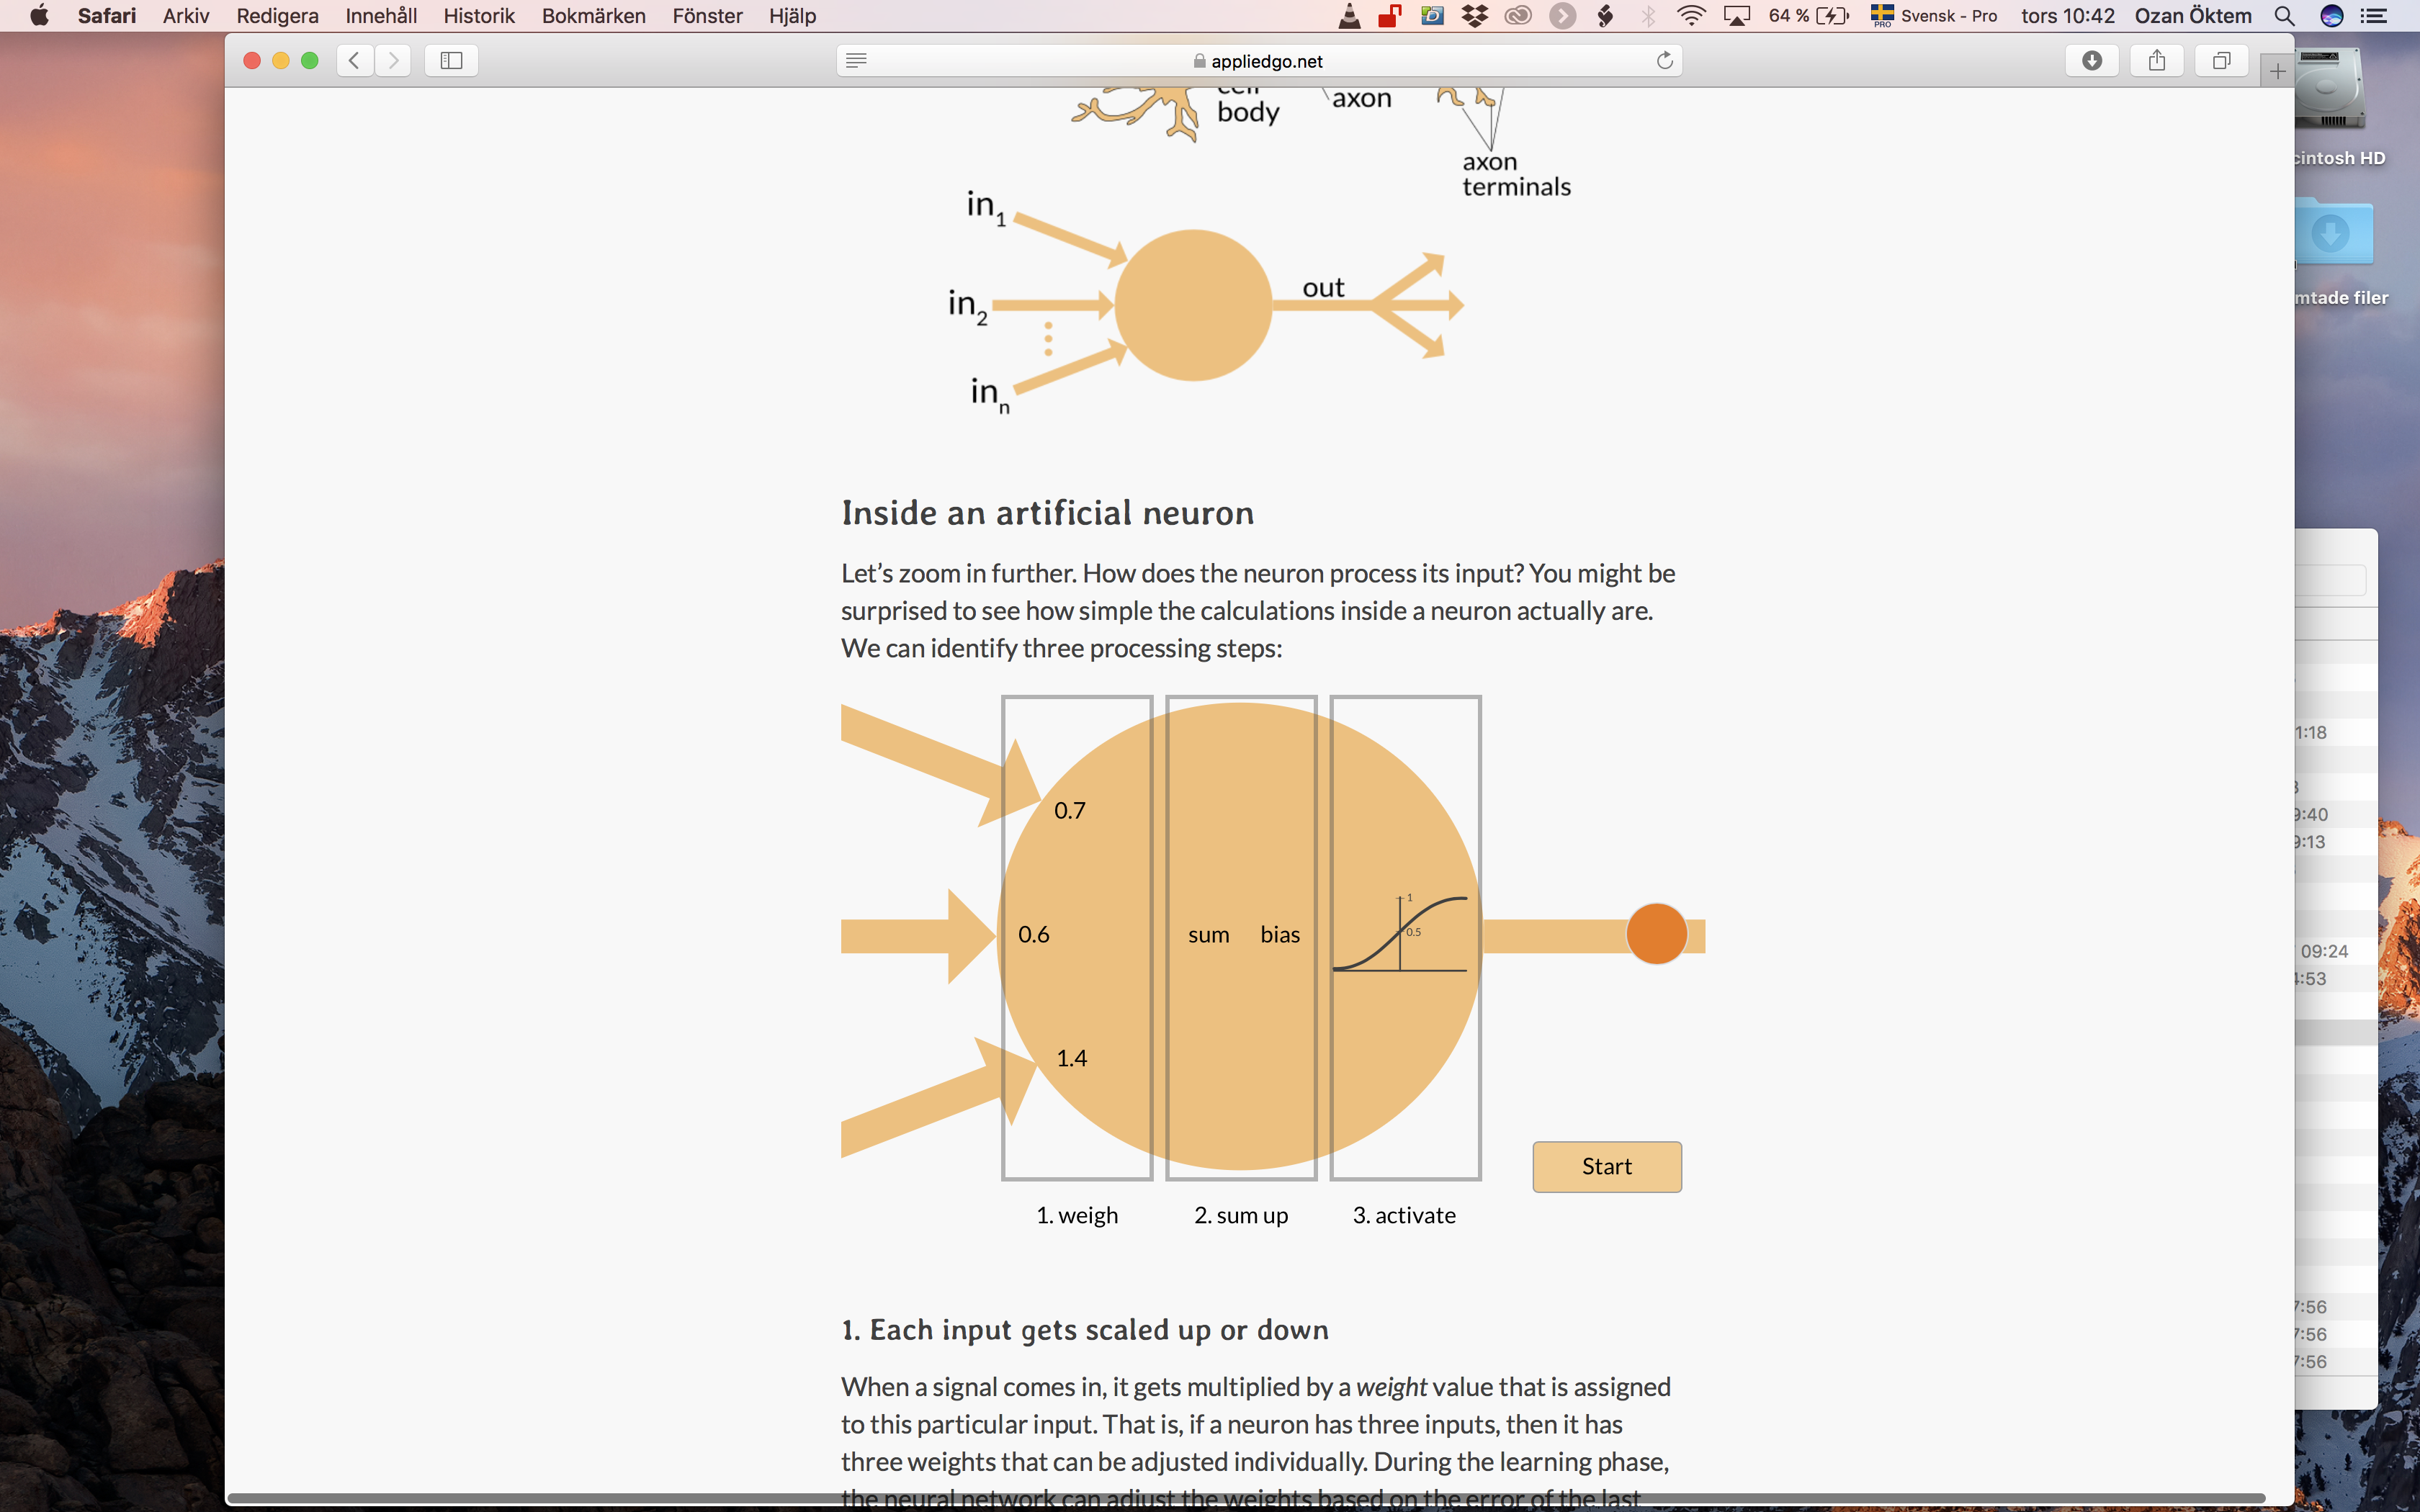
\includegraphics[trim={585 195 495 483},clip,height=0.9\textheight]{step9}
%\end{overprint}
%\end{center}
%\end{frame}


% Frame
\begin{frame}{Sequential deep network}
$\model \colon \Real^n \to \Real^m$ where $\model := \model_{\depth} \circ \ldots \circ \model_{1}$:
\begin{itemize}
\visible<2->{
\item \structure{Perceptron:} $\model_{k} \colon \Real^{\layerdim_{k-1}} \to \Real^{\layerdim_{k}}$ with $\model_{k} := \NonLinMap_k \circ \LinMap_{k}$
  and $\layerdim_{1}:=n$ \& $\layerdim_{\depth}:=m$.
  \begin{itemize}
  \item \structure{Depth:} $\depth \in \Natural$.   
  \item \structure{Affine linear map:}  $\LinMap_{k} \colon \Real^{\layerdim_{k-1}} \to \Real^{\layerdim_{k}}$ given by 
    \[ \LinMap_{k}(x) := \NNMatrix_k \cdot x+b_k  \quad\text{for $k=2,\ldots,\depth$} \]
    with $\NNMatrix_k \in \Real^{\layerdim_{k} \times \layerdim_{k-1}}$ (weights) and $b_k \in \Real^{\layerdim_{k}}$ (bias).
  \item \structure{Activation:} 
    $\NonLinMap_k(\inputvar_1, \ldots, \inputvar_{\layerdim_k}) 
      := \bigl( \Activation_k(\inputvar_1), \ldots, \Activation_k(\inputvar_{\layerdim_k}) \bigr)$
    given $\Activation_k \colon \Real \to \Real$ (activation function/rectifier).
  \end{itemize}
}
\visible<3->{
\item \structure{Intermediate layer:} Output of multiplication with $\NNMatrix_k$.
\item \structure{Dense/fully connected:} $\NNMatrix_{k}$ is a dense matrix with no a priori structure.
\item \structure{Connectivity:} Total number of nonzero weights.
\item \structure{Graph representation:} Represent $\model$ using a weighted \acf{DAG}, nodes (neurons) arranged in $\depth$ hierarchical layers and edges only between adjacent layers.
}
\end{itemize}
\end{frame}

% Frame
\begin{frame}{Sequential deep network}
\begin{itemize}
\item \structure{Classical representation:} Mappings from $k$:th to $(k+1)$:st layer:
\begin{center}
\tikzset{every neuron/.style={circle,draw,minimum size=1cm},
  neuron missing/.style={draw=none,scale=4,text height=0.333cm,execute at begin node=\color{black}$\vdots$},
}
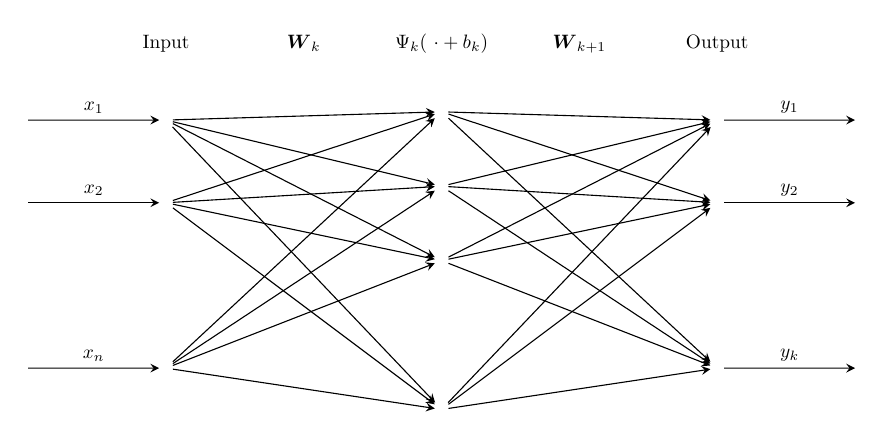
\begin{tikzpicture}[x=2.5cm, y=1.5cm, >=stealth,scale=0.7, every node/.style={scale=0.7}]
\foreach \m/\l [count=\y] in {1,2,missing,3}
\node [every neuron/.try, neuron \m/.try] (input-\m) at (0,2.5-\y) {};

\foreach \m [count=\y] in {1,2,3,missing,4}
\node [every neuron/.try, neuron \m/.try ] (hidden-\m) at (2,2.5-\y*0.9) {};

\foreach \m [count=\y] in {1,2,missing,3}
\node [every neuron/.try, neuron \m/.try ] (output-\m) at (4,2.5-\y) {};

\foreach \l [count=\i] in {1,2,\layerdim}
\draw [<-] (input-\i) -- ++(-1,0)
node [above, midway] {$x_{\l}$};

\foreach \l [count=\i] in {1,2,k}
\draw [->] (output-\i) -- ++(1,0)
node [above, midway] {$y_{\l}$};

% Linear map
\foreach \i in {1,...,3}
\foreach \j in {1,...,4}
\draw [->] (input-\i) -- (hidden-\j);

\foreach \i in {1,...,4}
\foreach \j in {1,...,3}
    \draw [->] (hidden-\i) -- (output-\j);

\foreach \l [count=\x from 0] in {Input, $\NNMatrix_{k}$, $\NonLinMap_k(\ \cdot + b_k)$, $\NNMatrix_{k+1}$, Output}
\node [align=center, above] at (\x,2) {\l \\ };
\end{tikzpicture}
\end{center}
\item \structure{Modern representation:}
\raisebox{-1.5ex}{%
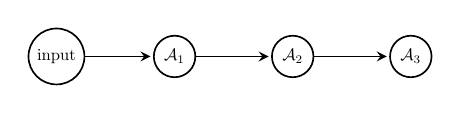
\begin{tikzpicture}[
> = stealth, % arrow head style
shorten > = 1pt, % don't touch arrow head to node
auto,
node distance = 2.5cm, % distance between nodes
semithick % line style
]

\tikzstyle{every state}=[scale=0.6, every node/.style={scale=0.6}]
draw = black,
thick,
fill = white,
minimum size = 4mm
]

\node[state] (inp) {input};
\node[state] (n1) [right of=inp] {$\model_{1}$};
\node[state] (n2) [right of=n1] {$\model_{2}$};
\node[state] (n3) [right of=n2] {$\model_{3}$};

\path[->] (inp) edge (n1);
\path[->] (n1) edge (n2);
\path[->] (n2) edge (n3);
\end{tikzpicture}
}
\end{itemize}
\end{frame}

% Frame
\begin{frame}{Non-Sequential networks}
	\begin{itemize}
		% Residual network
		\item \structure{Residual network:} Very successful/popular architecture, involves \emph{residual connections}.
		\par\medskip
		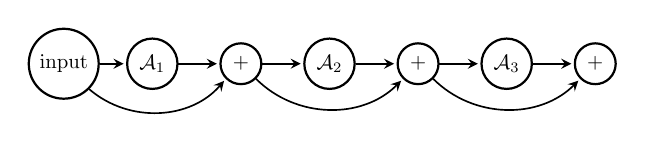
\begin{tikzpicture}[%
		> = stealth, % arrow head style
		shorten > = 1pt, % don't touch arrow head to node
		auto,
		node distance = 1.5cm, % distance between nodes
		semithick, % line style
		scale=0.75, every node/.style={scale=0.75} % scale
		]
		
		\tikzstyle{every state}=[
		draw = black,
		thick,
		fill = white,
		minimum size = 4mm
		]
		
		\node[state] (inp) {input};
		\node[state] (n1) [right of=inp] {$\model_{1}$};
		\node[state] (r1) [right of=n1] {$+$};
		\node[state] (n2) [right of=r1] {$\model_{2}$};
		\node[state] (r2) [right of=n2] {$+$};
		\node[state] (n3) [right of=r2] {$\model_{3}$};
		\node[state] (r3) [right of=n3] {$+$};
		
		% Linear
		\path[->] (inp) edge (n1);
		\path[->] (n1) edge (r1);
		\path[->] (r1) edge (n2);
		\path[->] (n2) edge (r2);
		\path[->] (r2) edge (n3);
		\path[->] (n3) edge (r3);
		
		% Residual
		\path[->] (inp) edge[bend right=45] (r1);
		\path[->] (r1) edge[bend right=45] (r2);
		\path[->] (r2) edge[bend right=45] (r3);
		\end{tikzpicture}
		% Dense network
		\item \structure{Dense network:} 
		Result from all previous layers are concatenated ($[\ ]$ indicates concatenation) to form the input to the next layer
		\par\medskip
		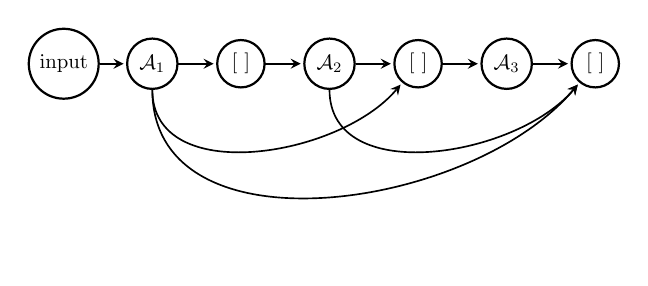
\begin{tikzpicture}[
		> = stealth, % arrow head style
		shorten > = 1pt, % don't touch arrow head to node
		auto,
		node distance = 1.5cm, % distance between nodes
		semithick, % line style
		scale=0.75, every node/.style={scale=0.75} % scale
		]
		
		\tikzstyle{every state}=[
		draw = black,
		thick,
		fill = white,
		minimum size = 4mm
		]
		
		\node[state] (inp) {input};
		\node[state] (n1) [right of=inp] {$\model_{1}$};
		\node[state] (r1) [right of=n1] {$[\ ]$};
		\node[state] (n2) [right of=r1] {$\model_{2}$};
		\node[state] (r2) [right of=n2] {$[\ ]$};
		\node[state] (n3) [right of=r2] {$\model_{3}$};
		\node[state] (r3) [right of=n3] {$[\ ]$};
		
		% Linear
		\path[->] (inp) edge (n1);
		\path[->] (n1) edge (r1);
		\path[->] (r1) edge (n2);
		\path[->] (n2) edge (r2);
		\path[->] (r2) edge (n3);
		\path[->] (n3) edge (r3);
		
		% Dense
		\path[->] (n1) edge[out=270, in=230] (r2);
		\path[->] (n1) edge[out=270, in=230] (r3);
		\path[->] (n2) edge[out=270, in=230] (r3);
		\end{tikzpicture}
		
		% Sparse network
		\item \vskip-\baselineskip
		\structure{Sparse network:} 
		Network architectures where most weights are zero, i.e., the connectivity is small relative to the number of connections possible.
	\end{itemize}
\end{frame}


% Frame
\begin{frame}{\Acf{CNN}}
	\structure{Idea:} Use \emph{geometry} of data (proximity, directions), suitable for \emph{images, volumes, graphs}.
	\begin{center}
		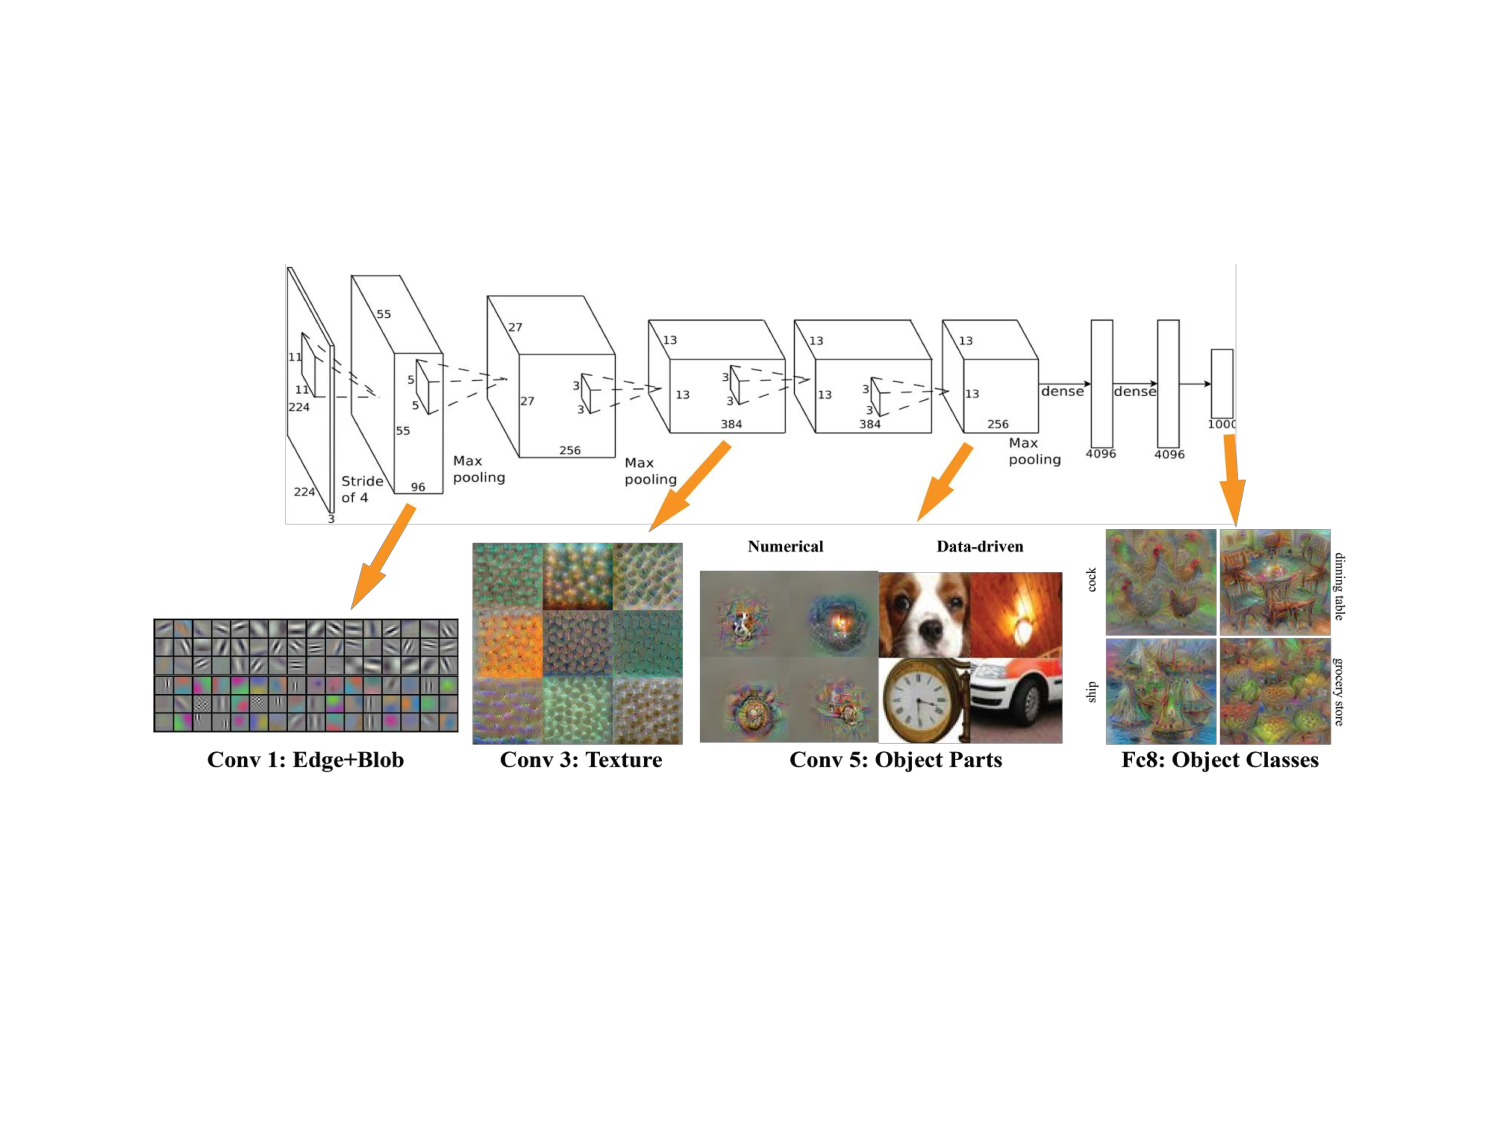
\includegraphics[width=0.7\textwidth]{CNN_layers2}
	\end{center}
% https://www.sciencedirect.com/science/article/pii/S2212671614000146
% We used Deep Convolutional Neural Network architecture, similar to (Krizhevsky et al., 2012), but trained on one GPU. It has 8 trainable layers, the first five of which are convolutional and other three are fully- connected (see Fig. 1). First, second and fifth convolutional layers are followed by max-pooling layers. First and second max-pooling layers are followed by local response normalization layers. We used Rectified Linear Units (ReLU) as neurons. First convolutional layer has 96 kernels of size 11x11x3 with a stride of 4 pixels. The second layer takes as input the max-pooled and response-normalized output of first layer and filters it with 256 kernels of size 5x5x48. The third convolutional layer takes as input the max-pooled and response- normalized output of the second layer and filters it with 384 kernels of size 3x3x256. The fourth layer has 384 kernels of size 3x3x192, and the fifth layer has 256 kernels of size 3x3x192. The fully-connected layers have 4096 neurons each. Max-pooling layers have size of 3x3 and stride of 2. The final layer is 1000-way Softmax.
	\structure{Layers:}
	Convolutional, Pooling
\end{frame}

% Frame
\begin{frame}{\Acf{CNN}}
	\begin{itemize}
		\item Suitable fort large-scale problems.
		\item Very good performance for various (approximately) translation invariant tasks.
		\item No clear and profound theoretical understanding explaining performance.
		%\item Final layer is a (sparse) representation \cite{Glorot:2011aa,Giryes:2016aa}. 
	\end{itemize}
	\visible<2->{
		Example procedure for feature extraction \cite{Zeiler:2013aa,Giryes:2016aa}:
		\begin{columns}[T]
			\begin{column}{0.45\textwidth}
				\begin{enumerate}
					\item Train \ac{CNN} to classify images.
					\item Features: Obtained from last layer (before classification), can be used to perform other tasks.
					\item Relevant information is `preserved' until the last layer.
				\end{enumerate}
			\end{column}
			\begin{column}{0.5\textwidth}
				\centering
				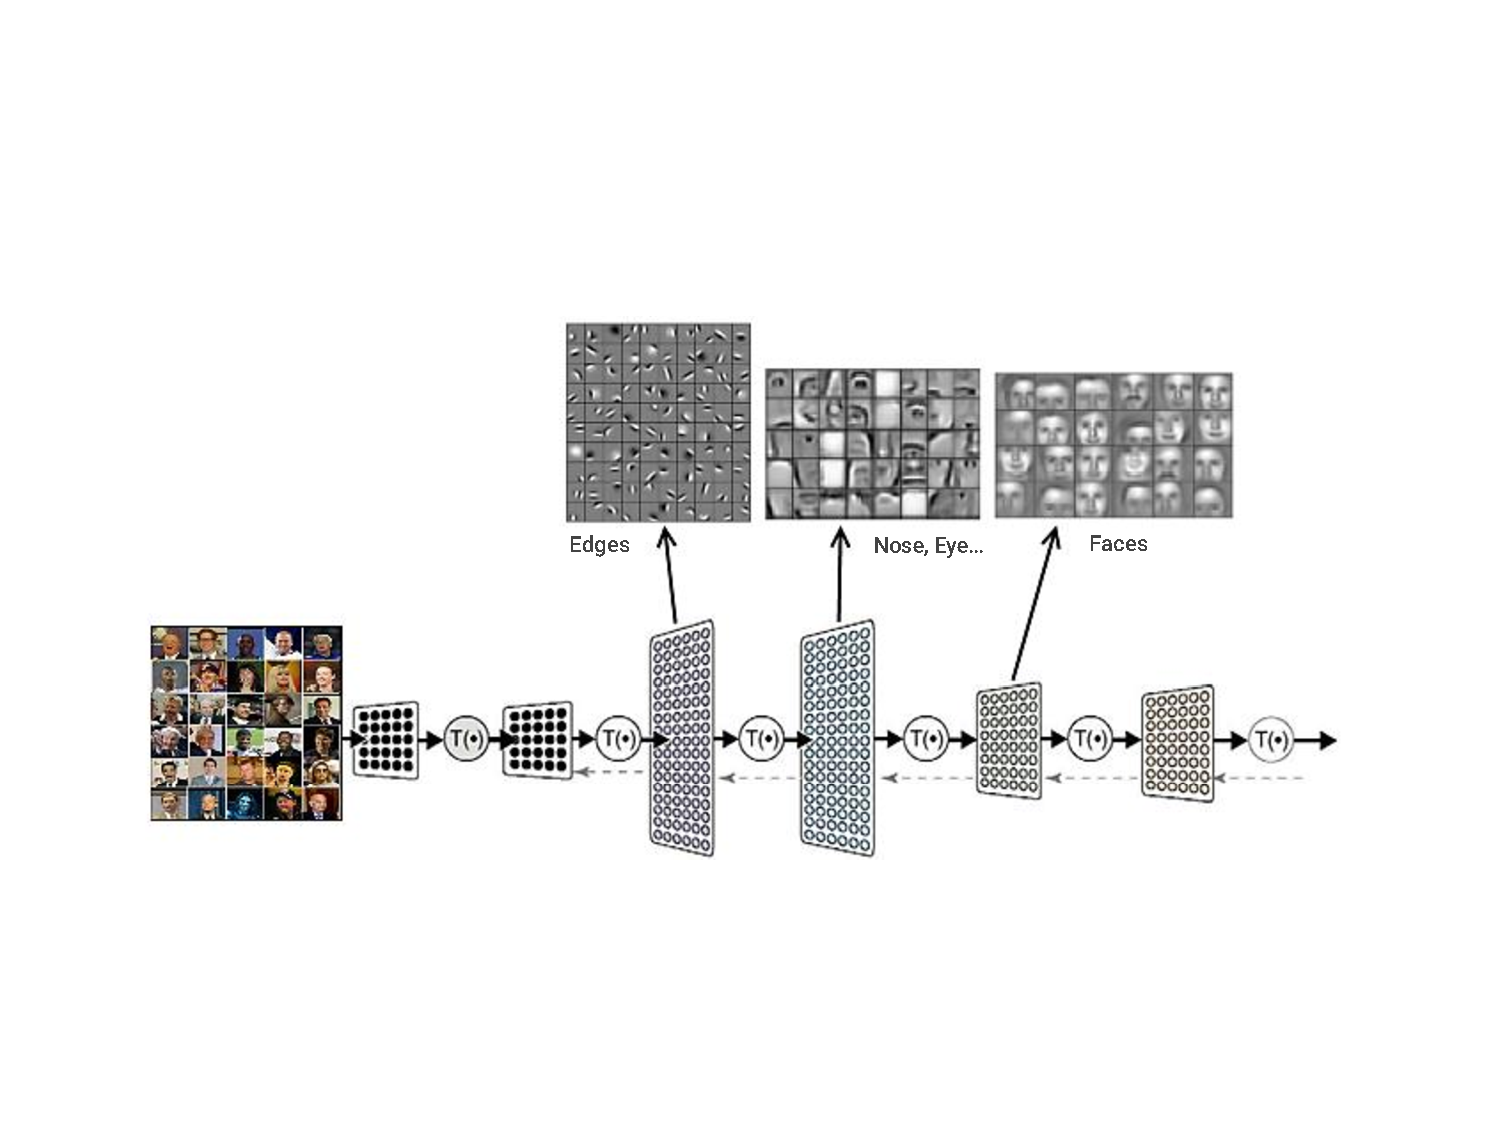
\includegraphics[width=\textwidth]{CNN_features}
			\end{column}
		\end{columns}
	}
\end{frame}

% Frame
\begin{frame}{\Acf{CNN}}
\structure{\Acf{CNN} components:}
\begin{itemize}
	\item Convolutional layers:
	\begin{itemize}
		\item Transposed convolutions.
		\item Strided convolutions.
	\end{itemize}
	\item Resizing:
	\begin{itemize}
		\item Downsampling by pooling (maxpooling, averagepooling).
		\item Upsampling (nearest neighbour, bi-linear).
	\end{itemize}
	\item Activation functions (ReLU, $\dots$)
	\item Regularization (Batch-Normalization, Dropout)
\end{itemize}
\end{frame}

\begin{frame}{\Acf{CNN}}
\structure{Convolutional layer:}
\begin{enumerate}
\item Data representation: Represent input/output as image with multiple channels (e.g. 3 for colour images, but typically $32$--$1024$ inside the network).
\item Definition: The input $\inputvar$ is transformed according to:
  \begin{itemize}
  \item $\iota =$ number of input channels.
  \item $\tau =$ number of output channels.
  \item $\LinMap_{i}(\inputvar) := \sum_{j=1}^{\iota} w_{i,j} \ast \inputvar + b_{i}$ for $i = 1, \ldots, \tau$.
  \\[0.25em]
  \item $\LinMap(\inputvar) :=  \bigl( \LinMap_{1}(\inputvar), \ldots, \LinMap_{\tau}(\inputvar) \bigr)$.
  \\[0.25em]
  \item $w_{i,j}$ is a convolution kernel, there are $\iota \tau$ such kernels.
  \item $b_i$ is the bias.
  \end{itemize}
\end{enumerate}
\end{frame}

% Frame
\begin{frame}{Deep \acf{RNN}}

\begin{itemize}
\item Usual neural networks: Input and output have fixed size, mapping has fixed parametrisation.
\item \Ac{RNN} architectures: No formal definition, but essential property is that it can map sequences in the input, output, or both by introducing connections between units that form a directed graph along a sequence.
\item Can learn arbitrary programs: Turing-complete, i.e., for every computable function there exists a finite \ac{RNN} (with an architecture from a simple class) that can compute it \cite{Siegelmann:1992aa}.
\\[0.25em]
\par\qquad
Training usual neural network $\Longleftrightarrow$ Optimisation over functions
\par\qquad
Training \ac{RNN} $\Longleftrightarrow$ Optimisation over programs
\item Memory: Information in the sequence itself. 
\end{itemize}
\end{frame}


% Frame
\begin{frame}{Deep \acf{RNN}}
\begin{center}
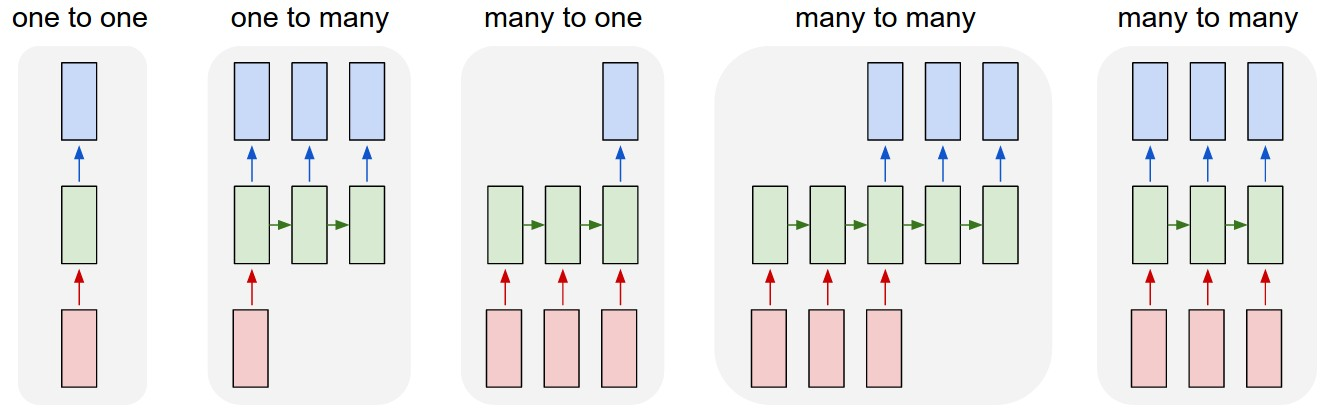
\includegraphics[height=0.4\textheight]{RRNs}
\begin{tikzpicture}[overlay]
  \visible<2>{\fill[red,fill opacity=0.1] (-9.3,0) rectangle (-8.1,3);}
  \visible<3>{\fill[red,fill opacity=0.1] (-7.9,0) rectangle (-6.3,3);}
  \visible<4>{\fill[red,fill opacity=0.1] (-6.2,0) rectangle (-4.5,3);}
  \visible<5>{\fill[red,fill opacity=0.1] (-4.4,0) rectangle (-1.8,3);}
  \visible<6>{\fill[red,fill opacity=0.1] (-1.7,0) rectangle (0,3);}
\end{tikzpicture}%
\end{center}
Input is red, output is blue, and green is intermediate layers. Intermediate layers fixed ny \ac{RNN} architecture, input and output may vary.
\begin{overprint}
\onslide<2> 
\begin{itemize}
\item Fixed-sized input and output, usual mode of processing without recurrent architecture.
\par
\structure{Example use case:} Image classification
\end{itemize}
\onslide<3> 
\begin{itemize}
\item Output is a sequence.
\par
\structure{Example use case:} Image captioning takes an image and outputs a sequence of words forming a sentence.
\end{itemize}
\onslide<4> 
\begin{itemize}
\item Input is a sequence.
\par
\structure{Example use case:} Sentiment analysis where a given sentence is classified as expressing positive or negative sentiment. 
\end{itemize}
\onslide<5> 
\begin{itemize}
\item Input and output are sequences.
\par
\structure{Example use case:} Machine Translation, a \ac{RNN} reads a sentence in English and then outputs a sentence in French.
\end{itemize}
\onslide<6> 
\begin{itemize}
\item Input and output are sequences that are synchronised (temporal linkage).
\par
\structure{Example use case:} Video classification (label each frame of a video). 
\end{itemize}
\end{overprint}
\end{frame}

% Frame
\begin{frame}{Zoo of architectures}
\centering
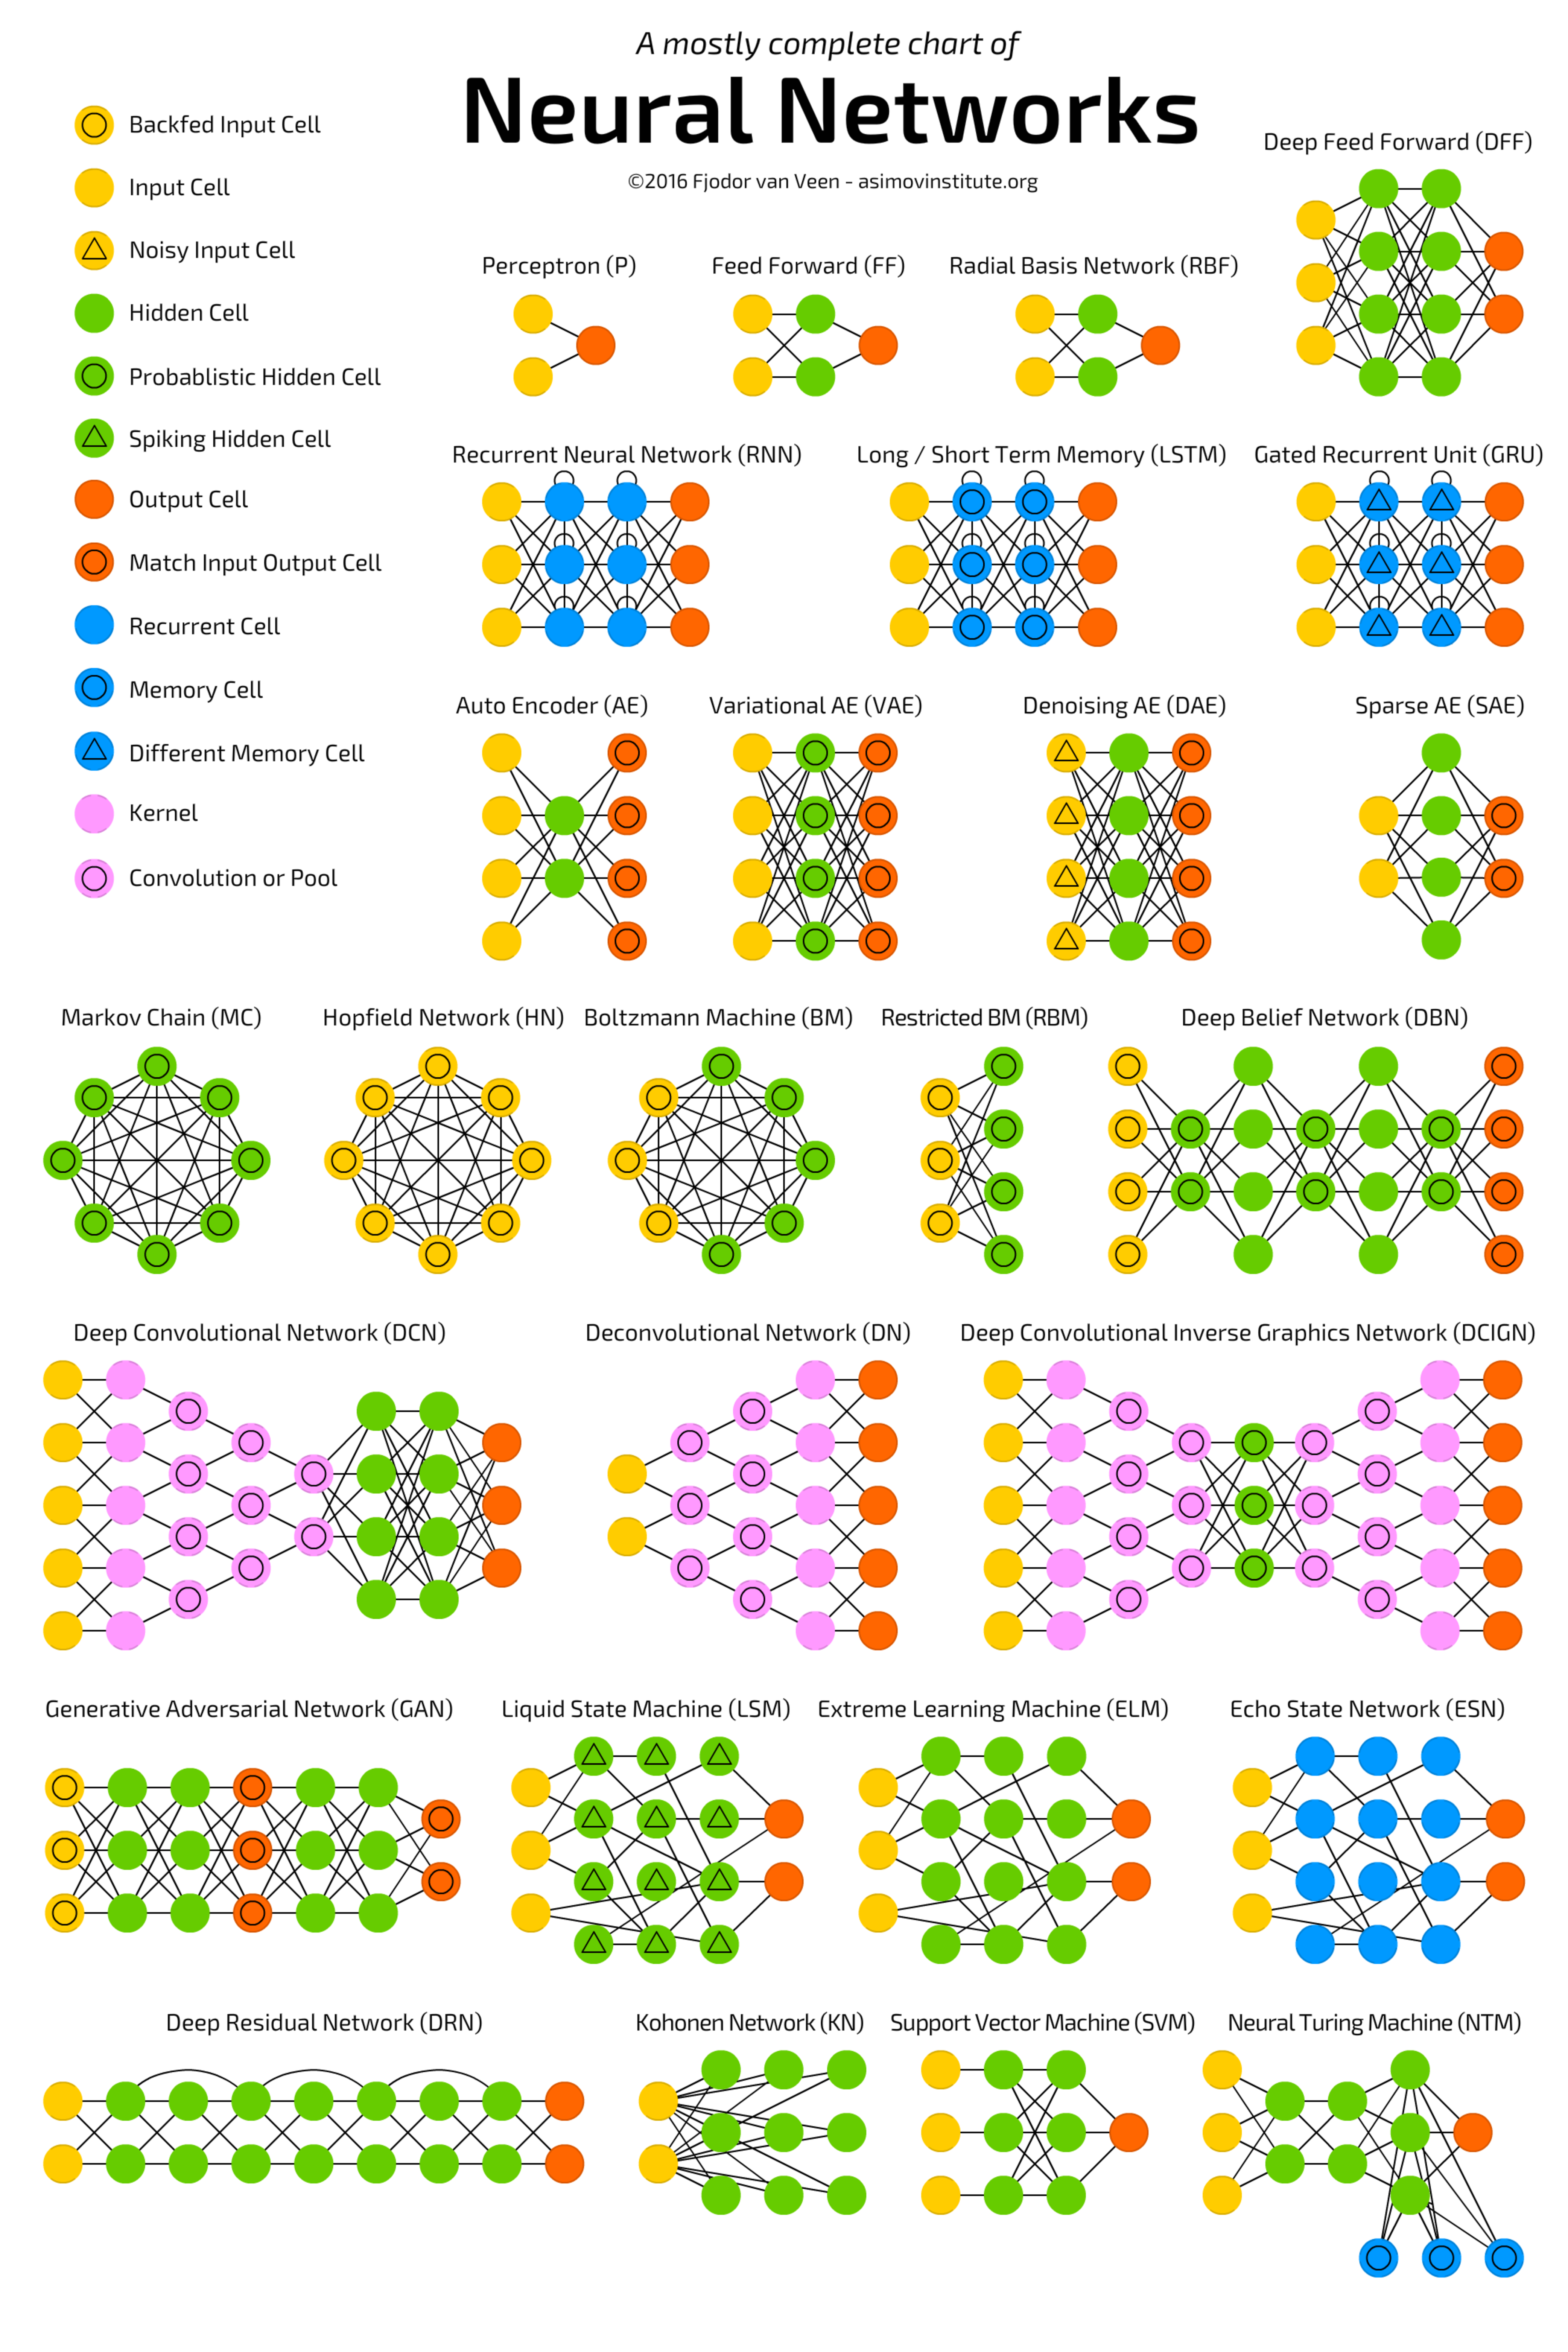
\includegraphics[height=\textheight]{NN_zoo}
\end{frame}


% Frame
\begin{frame}{Activation functions}{Some common choices}
\begin{overprint}
\onslide<1> % Slide 1
\begin{columns}[T]
\begin{column}{0.3\textwidth} % Column 1
  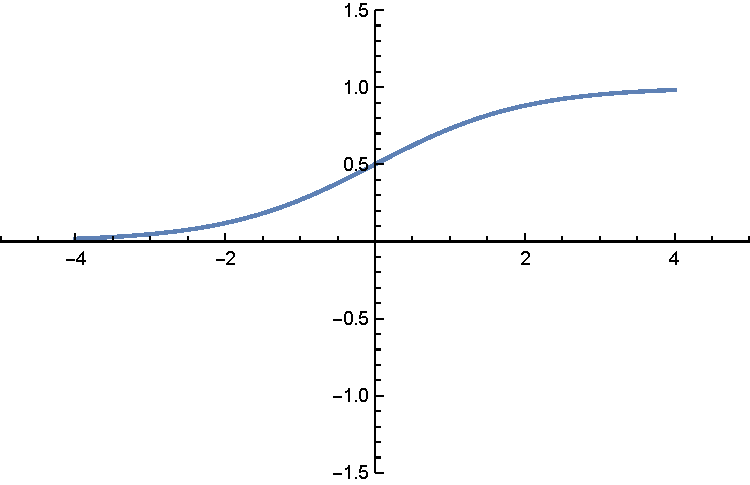
\includegraphics[width=\textwidth]{Logistic}
  \par
  {\small
  \structure{Logistic}
  \[ \Activation(t) := \frac{1}{1+e^{-t}} \]}
\end{column}
\begin{column}{0.3\textwidth} % Column 2
  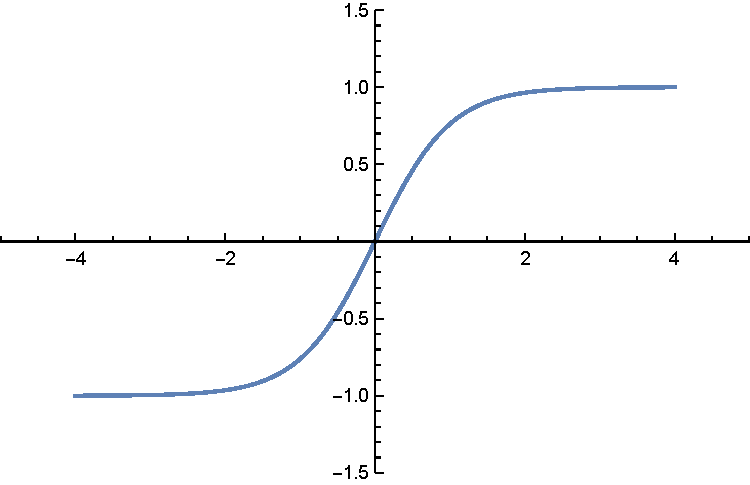
\includegraphics[width=\textwidth]{Tanh}
  \par
  {\small
  \structure{Tanh}
  \[ \Activation(t) := \tanh(t) \]}
\end{column}
\begin{column}{0.3\textwidth} % Column 3
  \includegraphics[width=\textwidth]{SoftSign}
  \par
  {\small
  \structure{Softsign}
  \[ \Activation(t) := \frac{t}{1+ | t |} \]}
\end{column}
\end{columns}
\onslide<2> % Slide 2
\begin{columns}[T]
\begin{column}{0.3\textwidth} % Column 1
  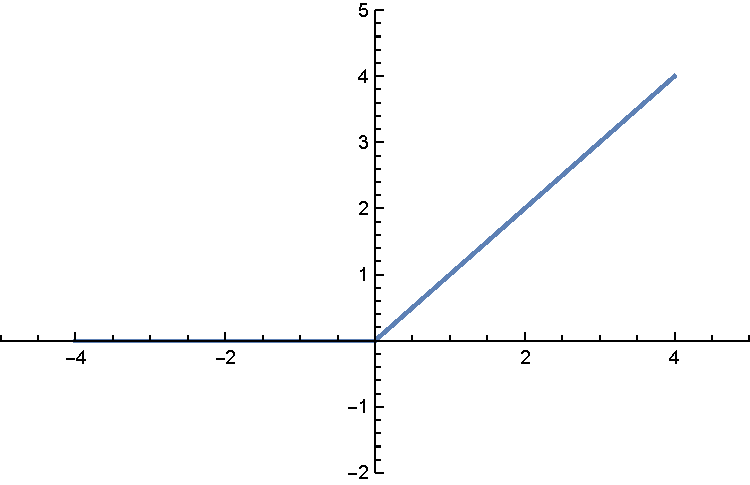
\includegraphics[width=\textwidth]{ReLU}
  \par
  {\small
  \structure{\Acf{ReLU}}
  \[ \Activation(t) := \begin{cases} 0 &\text{if $t <0$}  \\ t & \text{otherwise} \end{cases} \]}
\end{column}
\begin{column}{0.3\textwidth} % Column 2
  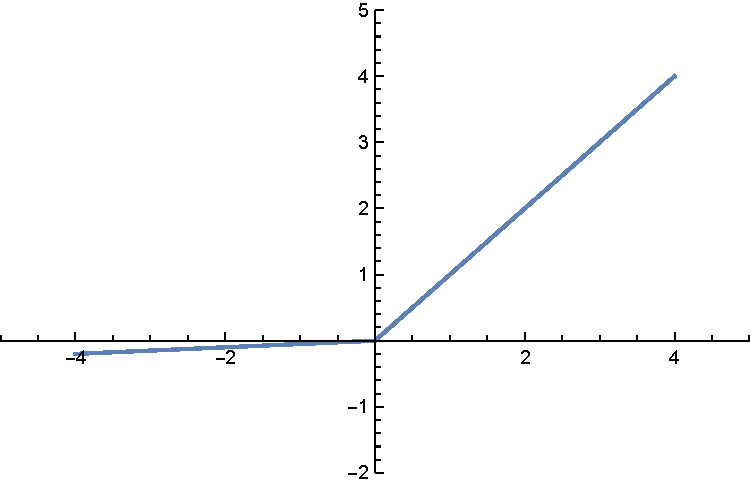
\includegraphics[width=\textwidth]{LeakyReLU}
  \par
  {\small
   \structure{Leaky \ac{ReLU}}
   \[ \Activation(t) := \begin{cases} \epsilon t &\text{if $t <0$}  \\ t & \text{otherwise} \end{cases} \]
   with $0 < \epsilon \ll 1$.}
\end{column}
\begin{column}{0.3\textwidth} % Column 3
  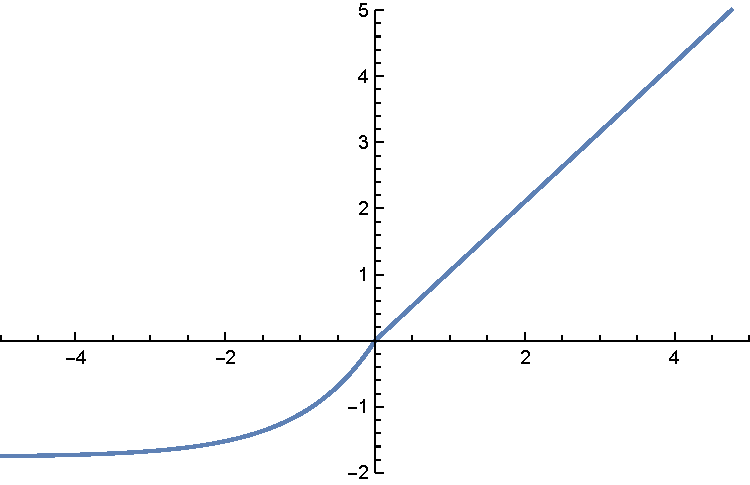
\includegraphics[width=\textwidth]{SELU}
  \par
  {\small
   \structure{Scaled exponential linear unit (SELU)}
   \[ \Activation(t) := \begin{cases} \lambda t &\text{if $t >0$}  \\ \lambda \alpha(e^t-1) & \text{otherwise} \end{cases} \]
   $\lambda \approx 1.0507$ and $\alpha \approx 1.6732$ for standard scaled input (mean 0, stddev 1).}
\end{column}
\end{columns}
\onslide<3> % Slide 3
Almost all deep neural networks use \ac{ReLU} (or a variant of it), since it trains much faster, is more expressive than logistic function and seems to have a regularising property.
\end{overprint}
\end{frame}

%% Frame
%\begin{frame}{Network architectures}{Activation functions: Some common choices}
%\begin{overprint}
%\onslide<1-6>
%\begin{columns}[T]
%\begin{column}{0.4\textwidth} % Column 1
%\begin{overprint}
%\onslide<1>
%  \structure{Heaviside (binary step) function}
%  \[ \Activation(t) := \begin{cases} 0 &\text{if $t <0$}  \\ 1 & \text{otherwise} \end{cases} \]
%\onslide<2>
%  \structure{Logistic (sigmoid or soft step)}
%  \[ \Activation(t) := \frac{1}{1+e^{-t}} \]
%\onslide<3>
%  \structure{Tanh}
%  \[ \Activation(t) := \tanh(t) = \frac{e^t-e^{-t}}{e^t+e^{-t}} \]
%\onslide<4>
%  \structure{Softsign}
%  \[ \Activation(t) := \frac{t}{1+ | t |} \]
%\onslide<5>
%  \structure{\Acf{ReLU}}
%  \[ \Activation(t) := \begin{cases} 0 &\text{if $t <0$}  \\ t & \text{otherwise} \end{cases} \]
%\onslide<6>
%  \structure{Leaky \ac{ReLU}}
%  \[ \Activation(t) := \begin{cases} \epsilon t &\text{if $t <0$}  \\ t & \text{otherwise} \end{cases} \]
%   with $0 < \epsilon \ll 1$.
%\end{overprint}
%\end{column}
%\hfill
%\begin{column}{0.57\textwidth} % Column 1
%\centering
%\begin{overprint}
%\onslide<1>
%  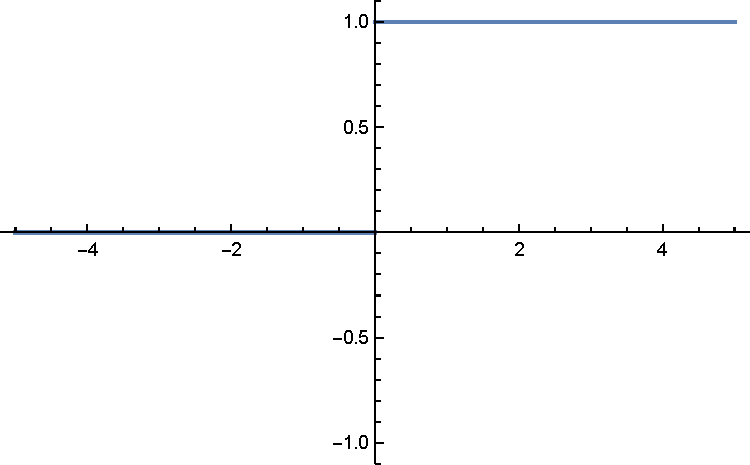
\includegraphics[width=\textwidth]{UnitStep}
%\onslide<2>
%  \includegraphics[width=\textwidth]{Sigmoid}
%\onslide<3>
%  \includegraphics[width=\textwidth]{Tanh}
%\onslide<4>
%  \includegraphics[width=\textwidth]{SoftSign}
%\onslide<5>
%  \includegraphics[width=\textwidth]{ReLU}
%\onslide<6>
%  \includegraphics[width=\textwidth]{LeakyReLU}  
%\end{overprint}
%\end{column}
%\end{columns}
%\end{overprint}
%\visible<5->{
%\par\bigskip
%Most deep networks use a variant of \ac{ReLU}, since it trains much faster, is more expressive than logistic function and seems to have a regularising property (prevents the gradient vanishing problem).
%}
%\end{frame}

% Frame
\begin{frame}{Further components of modern neural networks}
\begin{overprint}
\onslide<1> % Slide 1
\begin{itemize}
\item \structure{Dropout:}
  \begin{itemize}
  \item Replace selected layer $\model_{k} \colon \Real^{\layerdim_{k-1}} \to \Real^{\layerdim_{k}}$ with 
    \[ \widetilde{\model}_{k} := \Dropout_k \circ \model_{k} \]
    where $\Dropout_k \colon \Real^{\layerdim_{k}} \to \Real^{\layerdim_{k}}$ maps a random sub-space of $\Real^{\layerdim_{k}}$ to zero 
    and re-scales remaining nodes.
  \item Ensure to preserve average value across layers, e.g., if one has dropout rate $d$ then all values are scaled by $1/(1-d)$ to 
  preserve signal strength \cite{Hinton:2012aa,Dahl:2013aa,Srivastava:2014aa}.    
  \end{itemize}
\item \structure{Batch normalisation:}  % Batch normalisation
  Transform layer input so that it has zero mean and standard deviation one after applying the activation function \cite{Ioffe:2015ab}.
  \begin{itemize}
  \item Applies when activation function is equivariant to statistical normalisation (shift to zero-mean and unit variance), 
    which is the case with \ac{ReLU}.
  \item Further variants like layer normalisation \& instance normalisation.
  \end{itemize}
\end{itemize}
\onslide<2> % Slide 2
\begin{itemize}
\item \structure{Pooling:} % Pooling
  Add layers and associated operators that summarise `nearby' nodes.
  \begin{itemize}
  \item Replace $\NonLinMap_k \colon \Real^{\layerdim_{k}} \to \Real^{\layerdim_{k}}$ with 
    \[ \Pool_k \circ \NonLinMap_k \colon \Real^{\layerdim_{k}} \to \Real^{\layerdim'_{k}}. \] 
  \item \structure{Pooling operator:} 
    $\Pool_k \colon \Real^{\layerdim_{k}} \to \Real^{\layerdim'_{k}}$ maps `nearby' nodes in 
    $\Real^{\layerdim_{k}}$ to a single node in $\Real^{\layerdim'_{k}}$.
    Requires a notion of `proximity' between nodes.
  \item \structure{Max pooling:} Maximum value of each cluster \cite{Ciregan:2012aa}.
  \item \structure{$\ell_p$ pooling:} The $\ell_p$ norm of `clustered' nodes. 
  \end{itemize}
\item \structure{Unpooling:} % Strided convolution
  Upsample the image to higher resolution.
  \begin{itemize}
  \item Can be done in several ways (nearest neighbour, bi-linear, spline).
  \item Popular in fully convolutional networks.
  \item Approximately the adjoint of pooling.
  \end{itemize}
\end{itemize}
\onslide<3> % Slide 2
\begin{itemize}
	\item \structure{Strided convolution:} % Strided convolution
	Convolution kernel with jumps (strides, long steps).
	\begin{itemize}
		\item Can act as pooling, but more general (pooling operators expressible by convolutions).
		\item Corresponds to `learning how to summarise', whereas in pooling one pre-defines how the summary is performed. 
		\item Computationally more expensive.
		\item Also exists variants that preserve resolution (atrous/dilated convolution).
	\end{itemize}
	\item \structure{Transposed convolution:}
	Use convolution kernels that \textit{increase} resolution.
	\begin{itemize}
		\item Can act as unpooling.
		\item Corresponds to `learning how to interpolate'. 
		\item Computationally more expensive.
		\item Sometimes (erroneously) called deconvolution.
	\end{itemize}
\end{itemize}
\end{overprint}
\end{frame}


% Frame
\begin{frame}[plain]
\slideTitle{Properties of network architectures}
\begin{itemize}
\item Geometric stability
\item Model capacity
\item Learning as an inverse problem
\end{itemize}
\end{frame}

%\begin{frame}{Basic notions}
%\begin{itemize}
%\item \structure{Model capacity:}
%  Characterise $\OutputSpace$-valued measurable maps on $\InputSpace$ that can be approximated arbitrarily well by an element in 
%  $\{ \model_{\param} \}_{\param}$ given sufficient training data.
%\item \structure{Learning:}
%  Determine an `optimal' $\param$ so that $\model_{\param} \approx \model$ where $\model \colon \InputSpace \to \OutputSpace$ is 
%  known only through finitely many input-output sample points (training data).
%\item \structure{Stability of learning:}
%  Stability of the learning procedure w.r.t. variations in training data.
%\item \structure{Generalisation:}
%  Does $\model_{\param} \approx \model$ also hold for unseen data, e.g., is the trained map itself stable?
%\item \structure{Interpretability:}
%  Is it possible to interpret components of the map $\model_{\param} \colon \InputSpace \to \OutputSpace$?
%\end{itemize}
%\end{frame}


% Frame
\begin{frame}{Geometric stability}{Invariance \& equivariance}
\begin{itemize}
\item Many tasks invariant to the action of transformation groups (translations, rotations, frequency transpositions).
\item Neural network architectures should provide models that exhibit same invariances.
\item Transformation group $G$ with (left) action on both $\InputSpace$ and $\OutputSpace$:
  \begin{itemize}
  \item \structure{Invariance under $G$:} $\model(g.\inputvar) = \model(\inputvar)$.
  \item \structure{Equivariance under $G$:} $\model(g.\inputvar) = g.\model(\inputvar)$.
  \end{itemize}
\item \structure{Translation invariance (stationarity) \cite{Mallat:2012aa}:} 
  \begin{itemize}
  \item $G$ is group of translations, i.e., elements $g(\tau) := \tau-\nu$ for some $\nu \in \Real^k$. 
  \item Action on $\inputvar$ is $g.\inputvar := \inputvar \circ g$.
  \item Invariance: $\model(\inputvar \circ g) = \model(\inputvar)$ 
  \item Equivariance: $\model(\inputvar \circ g) = g' \circ \model(\inputvar)$ where $g,g' \in G$ are translation operators on appropriate space.
  \item Translation invariant tasks: Object classification, modulus of the Fourier transform.
  \item Translation equivariant tasks: Object localisation, semantic segmentation, motion estimation, tomographic reconstruction.
\end{itemize}
\end{itemize}
\end{frame}

% Frame
\begin{frame}{Geometric stability}{Local deformations and scale separation}
\begin{itemize}
\item Information content in many signals (sound, images) typically stable under action of other groups, e.g., small diffeomorphisms \cite{Trouve:2005aa}.
  \par $\implies$ Need model that is stable under such deformations.
\item Instabilities to diffeomorphic deformations are well-known to appear at high frequencies \cite{Hormander:1971aa}. 
  Translation invariant operators are not Lipschitz continuous w.r.t. the action of diffeomorphisms (difficult to maintain Lipschitz continuity over high frequencies).
  \par $\implies$ Network having same invariance (e.g., translation invariance) as task is in general not enough. 
\item Model needs to be nonexpansive to preserve stability.
  \par $\implies$ Sufficient to verify its Lipschitz continuity under action of small diffeomorphisms close to translations (linearised diffeomorphisms).
\end{itemize}
\end{frame}

% Frame
\begin{frame}{Geometric stability}{Local deformations and scale separation}
\begin{itemize}  
\item $G$ group of $g_{\nu}(\inputvar) := \inputvar - \nu(\inputvar)$ for some smooth vector field $\nu \colon \Real^k \to \Real^k$.  
  If $\nu$ small, then $g_{\nu}$ is invertible. 
  \par $\implies G \subset$ diffeomorphisms (linearised diffeomorphisms).
\item Group action: $g_{\nu}.\inputvar := \inputvar \circ g_{\nu}$, i.e., $g_{\nu}.\inputvar(\tau) = \inputvar(\tau-\nu(\tau))$.
\item \structure{Local deformations \& scale separation:} 
  \par  Lipschitz stability: $\Vert\model(\inputvar)-\model(g_{\nu}.\inputvar) \Vert$ is bounded by the `size' of the diffeomorphism $g_{\nu}$
           up to a multiplicative constant multiplied by $\Vert \inputvar \Vert$.
  \par  Size of diffeomorphism $g_{\nu} \implies$ distance between $g_{\nu}$ and $\Id \implies \Vert \nu \Vert$. 
  \par Stability: $\Vert\model(\inputvar)-\model(g_{\nu}.\inputvar) \Vert$ bounded by $\Vert \nu \Vert$.
\end{itemize}
\end{frame}

% Frame
\begin{frame}{Geometric stability}{Architectures that exhibit invariance and stability}
\begin{itemize}
\item \structure{\Acp{CNN}}
  \begin{itemize}
  \item Translation invariant and stable w.r.t. local deformations and scale separation.
  \item Invariance can be cast as a form of stable group invariance. 
  \item Network architecture determines the invariance group, while trainable filter coefficients characterise the group action \cite{Bruna:2013ab}. 
  \end{itemize}
\item \structure{Scattering networks} \cite{Mallat:2012aa,Bruna:2013aa,Mallat:2016aa}
  \begin{itemize}
  \item Replace learned filters in the \ac{CNN} with predefined Wavelet functions given by cascading complex wavelet 
    modulus operators with a lowpass smoothing kernel.
  \item Provably stable and locally invariant (translations and rotations).
  \item Reveal the fundamental role of geometry and stability that underpins the generalisation performance of modern deep convolutional 
    network architectures.
  \end{itemize}
\end{itemize}
\end{frame}
 
% Frame
\begin{frame}{Model capacity}{The XOR affair}

\structure{Model capacity:}
  Characterise $\OutputSpace$-valued measurable maps on $\InputSpace$ that can be approximated arbitrarily well by an element in 
  $\{ \model_{\param} \}_{\param}$ given sufficient training data.
\par\bigskip
\visible<2->{  
\begin{block}{The XOR affair \shortcite{Minsky:1969aa}}
A feed-forward network with a single intermediary layer cannot replicate the exclusive-or (XOR) logic mapping unless at least one node the intermediate layer is connected with a non-zero weight to each and every input node.
\end{block}
\begin{itemize}
\item Resulting in funding cuts for neural networks. 
\item Was known that a multilayer perceptron easily replicates the XOR logic mapping.
\end{itemize}
}
\end{frame}


% Frame
\begin{frame}{Model capacity}{Universal approximation theorem}
\begin{block}{Universal approximation theorem \cite{Cybenko:1989aa,Hornik:1991aa,Pinkus:1999aa}}
Let $A \colon \Omega \to \Real$ be Borel measurable where $\Omega \subset \Real^n$ is compact and $\Activation \colon \Real \to \Real$ is continuous and not a polynomial. Then, for each $\epsilon > 0$ there exist $N \in \Natural$, $a_k,b_k \in \Real$, and $w_k \in \Real^n$ such that
\vskip-1.5\baselineskip
\[ 
   \biggl\Vert A - \sum_{k=1}^N a_k \Activation\bigl( \langle w_k, \,\cdot\, \rangle - b_k \bigr) \biggr\Vert_{\infty} \leq \epsilon.
\]
\end{block}
\begin{overprint}
\onslide<1> % Interpretation &. Historical notes
\begin{itemize}
\item \structure{Large model capacity:} 
The theorem implies that (deep) neural networks have large model capacity since they can uniformly approximate any Borel measurable function arbitrarily well.
%Every Borel measurable function can be approximated up to an error of $\epsilon>0$ with a single layer feed-forward neural network with finite number of nodes.
\item George Cybenko \cite{Cybenko:1989aa} proved result for sigmoid activation functions.
\item Kurt Hornik \cite{Hornik:1991aa} showed that the critical property is the multilayer feedforward architecture rather than the choice of activation function.
\end{itemize}
\onslide<2> % Model capacity vs. network architecture
\begin{itemize}
\item \structure{Network architecture:} Choice of $N \in \Natural$ and $\Activation \colon \Real \to \Real$.
\item \structure{Learning:} Determine $a_k, b_k \in \Real$ and $w_k \in \Real^n$ from training data.
\end{itemize}
What is the connection between $\epsilon$ and network architecture (choice of $N$ and $\Activation$)?
\begin{center}
Model capacity $\longleftrightarrow$ Complexity of approximating neural network
\end{center}
\end{overprint}
\end{frame}


% Frame
\begin{frame}{Model capacity}{Capacity vs. complexity}
\begin{itemize}
\item \structure{Goal:} Bound complexity of \ac{ReLU} networks that approximate classifier functions.
\item \structure{Classifier function:} A function whose range is a finite set in $\Real$. 
\item \structure{$\beta$-regular classifier:} Any finite linear combination of characteristic functions of sets in $\Real^n$ with $C^\beta$-boundary.
\end{itemize}
\vskip-\baselineskip
\begin{overprint}
\onslide<1>
\begin{block}{Theorem \cite{Yarotsky:2017aa}  } 
Any $\beta$-regular classifier function on $\Real^n$ can be approximated up to accuracy $\epsilon >0$ in $L^\infty$-norm by a \ac{ReLU} network with at most 
\begin{itemize}
\item $C \epsilon^{-n/\beta}(\log_2(1/\epsilon)+1)$ non-zero weights and nodes, and
\item depth $C (\log_2(1/\epsilon)+1)$.
\end{itemize}
\end{block}
\begin{itemize}
\item Depth of \ac{ReLU} network depends on $\epsilon$.
\end{itemize}
\onslide<2>
\begin{block}{Theorem \cite{Petersen:2017aa}}
Any $\beta$-regular classifier function on $\Real^n$ can be approximated up to accuracy $\epsilon >0$ in $L^2$-norm by a \ac{ReLU} network with at most 
\begin{itemize}
\item $C \epsilon^{-n/\beta}$ non-zero weights, and
\item $C' (1+\beta/n) \log_2(2+ \beta)$ layers.
\end{itemize}
\end{block}
\begin{itemize}
\item Depth of \ac{ReLU} network independent of $\epsilon$.
\item Results extends to other functions classes relevant for signal processing.
\end{itemize}
\end{overprint}
\end{frame}

%% Frame
%\begin{frame}{Model capacity}{Optimal rates of approximation}
%%\begin{block}{Theorem \cite{Maiorov:1999aa}}
%%There exists a neural network of fixed size with an analytic and strictly increasing activation function $\Activation \colon \Real \to \Real$ where 
%%\[ \lim_{x\to -\infty} \Activation(x)=0 \quad\text{and}\quad 
%%   \lim_{x\to \infty} \Activation(x)=1
%%\]
%%that can approximate any continuous function arbitrarily well.
%%\end{block}
%Theorems concerning rates of convergence.
%\begin{itemize}
%\item None in the general setting \cite{Maiorov:1999aa}.
%\item Results require:
%  \begin{itemize}
%  \item Restrict activation function (e.g. consider only \ac{ReLU}) 
%  \par $\implies$ model complexity bounds.
%  \item Restrict the weights $\implies$ information theoretical bounds.
%  \item Other notions of model complexity 
%  \par $\implies$ continuous $N$-widths \shortcite{Bolcskei:2017aa}:
%   \visible<2->{%
%   \begin{itemize}
%   \item Optimal approximation rates of \ac{ReLU} networks for various classifier functions, like (piecewise) smooth functions.
%   \item Smoother functions allow better approximation rates, but achieving these rates requires deeper networks!
%   \item Relies heavily on theory from computational harmonic analysis.
%   \item Results only for real valued functions.
%   \end{itemize}}
%  \end{itemize}
%\end{itemize}
%\end{frame}


% Frame
\begin{frame}{Learning as an inverse problem}
\begin{itemize}
\item \structure{Goal:} Estimate $\model \colon \InputSpace \to \OutputSpace$ given 
  $(\stinputvar,\stoutputvar) \sim \alert<4>{\mu}$ where $\stoutputvar \approx \model(\stinputvar)$.
\\[0.5em]
\item \structure{Network architecture:} Specifies model class $\{ \model_{\param} \}_{\param}$ 
  with $\model_{\param} \colon  \InputSpace \to \OutputSpace$.
\\[0.5em]
\item \structure{\alt<5-7>{Empirical risk}{Risk}:} Given distance notion $\loss_{\OutputSpace} \colon \OutputSpace \times \OutputSpace \to \Real$,
\vskip-0.5\baselineskip
\begin{overlayarea}{\linewidth}{2\baselineskip}
\[ 
  \alt<5-7>%
    {\Risk_{\alert<5>{\tmu}}(\param) := \Expect_{\alert<5>{\tmu}}\Bigl[ \loss_{\OutputSpace}\bigl(\model_{\param}(\inputvar),\stoutputvar\bigr) \Bigr]}
    {\Risk_{\alert<4>{\mu}}(\param) := \Expect_{\alert<4>{\mu}}\Bigl[ \loss_{\OutputSpace}\bigl(\model_{\param}(\inputvar),\stoutputvar\bigr) \Bigr]}. 
\] 
\end{overlayarea}  
\item \structure{Decision problem:}   
\alt<5-7>{Find $\model_{\optimParamEmp} \colon  \InputSpace \to \OutputSpace$ where $\optimParamEmp \in \Real^N$ minimises the empirical risk}%
{Find $\model_{\optimParam} \colon  \InputSpace \to \OutputSpace$ where $\optimParam \in \Real^N$ minimises the risk}:
\vskip-0.5\baselineskip
\begin{overlayarea}{\linewidth}{2.5\baselineskip}
\[ 
  \alt<5-7>%
  {\optimParamEmp \in \argmin_{\param\in \Real^N} \Risk_{\alert<5>{\tmu}}(\param) 
      = \argmin_{\param} \biggl\{ \frac{1}{m} \sum_{i=1}^m \Bigl[ \loss_{\OutputSpace}\bigl(\model_{\param}(\inputvar_i),\outputvar_i \bigr) \Bigr] \biggr\}}
  {\optimParam \in \argmin_{\param\in \Real^N} \Risk_{\alert<4>{\mu}}(\param) 
      = \argmin_{\param} \Expect_{\alert<4>{\mu}}\Bigl[ \loss_{\OutputSpace}\bigl(\model_{\param}(\inputvar),\stoutputvar\bigr) \Bigr]}.
\]
\end{overlayarea}      
\end{itemize}
\begin{overlayarea}{\textwidth}{7\baselineskip}
\begin{overprint}
\onslide<2-3>
\structure{Statistical interpretation:} 
Find the non-randomised decision rule that minimises the average risk (Bayes risk if $\stinputvar \sim \prior$ is known).
\\[0.5em]
\alt<2>%
{$\loss_{\OutputSpace} = L^2$-loss $\implies \model_{\optimParam}$ is the posterior mean \cite[Proposition~2.5.1]{Robert:2007aa}.
}
{$\loss_{\OutputSpace} =$ Bregman distance of a strictly convex non-negative differentiable functional $\iff \model_{\optimParam}$ is the posterior mean 
    \cite{Banerjee:2005aa}.
    \par
    Note: Bregman distance for $\inputvar \mapsto \langle \inputvar,\inputvar \rangle$ gives the $L^2$-loss. 
}
\onslide<4-5>
\structure{Issue:} Joint measure $\alert<4>{\mu}$ unknown, instead we have training data $(\inputvar_i,\outputvar_i) \in \InputSpace \times \OutputSpace$ for $i=1,\ldots,m$ 
that are (preferably i.i.d.) samples of $(\stinputvar,\stoutputvar)$.
\\[0.5em]%
\noindent\visible<5>{\structure{Solution:} Replace $\alert<5>{\mu}$ with the empirical measure $\alert<5>{\tmu := \sum_{i=1}^m \delta_{(\inputvar_i,\outputvar_i)}}$.}
\onslide<6>
\structure{Learning algorithm:} $\tmu \mapsto \model_{\param}$ where $\param \approx \optimParamEmp$.
\par\medskip
A learning algorithm maps training data to a model. This includes not only the network architecture but also methods, like early stopping, used to 
stabilise the method for solving the decision problem. Hence, it is only an approximation to the model that minimises the empirical risk.
\onslide<7>
\structure{Flat minima:} 
Small perturbations in the parameter space around a solution results in small changes in the objective.
\par $\implies \optimParamEmp$ varies slowly w.r.t. small perturbations to $\tmu$.
\end{overprint}
\end{overlayarea}
\end{frame}


% Frame
\begin{frame}{Learning as an inverse problem}
\structure{Decision problem:} Given network architecture $\{ \model_{\param} \}_{\param}$, need to compute 
\[ \optimParamEmp \in \argmin_{\param} \biggl\{ 
     \frac{1}{m} 
     \sum_{i=1}^m \Bigl[ \loss_{\OutputSpace}\bigl(\model_{\param}(\inputvar_i),\outputvar_i\bigr) \Bigr] 
   \biggr\}.
\]
\structure{Challenges:} Solving the decision problem is an inverse problem, is it well-posed? \visible<2->{\alert<2>{No!}}
\visible<2->{%
\begin{itemize}
\item Non-convexity (non-uniqueness)
\item Instability (generalises poorly, over-fitting, over-training, \ldots)
\end{itemize}
}

\visible<3->{%
\alert<3>{On the other hand, learned deep neural networks work remarkably well!}
\begin{block}{Generalisation (non-overfitting) puzzle}
Learned deep neural network models generalise well even when applied to problems where it is easy to come up with natural model architectures that generalise poorly. 
This absence of overfitting, despite large over-parametrisation leading to large model capacity, is a major puzzle.
%the latter demonstrated by zero training error on randomly labeled data
%
%A major puzzle in deep neural networks revolves around the absence of overfitting despite large over-parametrisation leading to large model capacity, the latter demonstrated by zero training error on randomly labeled data.
\end{block}
}
\visible<4->{\alert{Wherein lies the regularisation?}}
\end{frame}

% Frame
\begin{frame}{Learning as an inverse problem}{Adversarial attacks}
\begin{overprint}
\onslide<1>
\begin{itemize}
\item \structure{Adversarial attacks:} 
  Inputs to machine learning models that an attacker has intentionally designed to cause the model to make a mistake.
\item Robustness against such attacks crucial for building safe, widely distributed AI.
\end{itemize}
\onslide<2>
\begin{columns}
\hfill
\begin{column}{0.25\textwidth} 
  \includegraphics[width=\textwidth]{Panda}
  \par
  {\small `Panda' (57.7\%).}
\end{column}
\begin{column}{0.09\textwidth} 
  \vskip-3\baselineskip
  \[ +\,\,\, 0.07 \times \]
\end{column}
\begin{column}{0.25\textwidth} 
  \includegraphics[width=\textwidth]{Advesarial_noise}
  \par
  {\small Added distortion.}
\end{column}
\begin{column}{0.05\textwidth} 
  \vskip-3\baselineskip
  \[ = \]
\end{column}
\begin{column}{0.25\textwidth} 
  \includegraphics[width=\textwidth]{Panda}
  \par
  {\small `Gibbon' (99.3\%).}
\end{column}
\hfill
\end{columns}
\begin{itemize}
\item Adding a specific minimal distortion (=magnitude of the smallest bit of an 8 bit image encoding) changes GoogLeNet classification. \cite{Goodfellow:2015aa}. 
\item This attack requires access to the learning model (gradient of the empirical risk).
\item In case of small images, possible to design adversarial attack that only modifies one pixel \cite{Su:2018aa}!
\end{itemize}
\onslide<3>
\begin{columns}[T]
\begin{column}{0.23\textwidth} 
  \includegraphics[width=\textwidth]{Washer_dataset}
  \par
  {\small Image from dataset.}
\end{column}
\begin{column}{0.23\textwidth} 
  \includegraphics[width=\textwidth]{Washer_photo}
  \par
  {\small Photo of printout of image from dataset. \par 54.0\% `washer'}
\end{column}
\begin{column}{0.23\textwidth} 
  \includegraphics[width=\textwidth]{Washer_advesarial_1}
  \par
  {\small Photo + distortion \par 34.6\% `safe' \par 22.0\% `washer'}
\end{column}
\begin{column}{0.23\textwidth} 
  \includegraphics[width=\textwidth]{Washer_advesarial_2}
  \par
  {\small Photo + distortion \par 37.2\% `safe' \par 24.2\% `loudspeaker'}
\end{column}
\end{columns}
\begin{itemize}
\item \structure{Black box attack:} Can construct adversarial attack without access to the learning model \cite{Papernot:2017aa}.
\item Above example shows black box attack from distorting photos of printed images \cite{Kurakin:2017aa}.
\end{itemize}
\end{overprint}
\end{frame}

% Frame
\begin{frame}{Summary}
Active research field: Relate network architecture to
\begin{itemize}
\item Model capacity
\item Model complexity
\item Stability during learning
\item Generalisation properties
\item Computational feasibility
\item Interpretability
\end{itemize}
Most efforts focus on the generic setting, i.e., all information is contained in training data.
\end{frame}

% Frame
\begin{frame}[plain]
\slideTitle{Generalisation}
\begin{itemize}
\item Type of errors related to learning
\item Practical role
\item Estimating the generalisation gap
\item Rethinking generalisation
\end{itemize}
\structure{Main reference:} \cite{Kawaguchi:2018aa}
\end{frame}

% Frame
\begin{frame}{Types of errors related to learning}
\begin{itemize}
\item \structure{Learning algorithm:} $\tmu \mapsto \model_{\param} \colon \InputSpace \to \OutputSpace$ where $\param \approx \optimParamEmp$ minimises the empirical risk.
\\[0.5em]
\item
\structure{Training error:} 
$\trainError := \Risk_{\tmu}(\optimParamEmp) =
      \Expect_{\tmu}\Bigl[ \loss_{\OutputSpace}\bigl( \model_{\optimParamEmp}(\stinputvar), \stoutputvar \bigr) \Bigr].
$      
\\[0.5em]
\item \structure{Test error:} 
Risk associated with the learned model when evaluated against a (test) measure $\eta$ on $\InputSpace \times \OutputSpace$:
\[
  \epsilon_{\eta} := \Expect_{\eta}\Bigl[ \loss_{\OutputSpace}\bigl( \model_{\optimParamEmp}(\stinputvar), \stoutputvar \bigr) \Bigr].
\]
\item \structure{Empirical test (validation) error:} Test error with $\eta :=$ empirical measure of test/validation data.
\item \structure{Expected risk/error:} Test error with $\eta :=\mu$ (full joint measure).
%\item \visible<3->{%
%\structure{Generalisation gap (error):} Given $(\mu,\tmu)$ and a learned model $\model_{\optimParamEmp} \in \ModelClass$, it is the difference between expected error and training error:
%\[ \genError := \epsilon_{\mu} - \trainError =
%   \Expect_{\mu}\Bigl[ \loss_{\OutputSpace}\bigl( \model_{\optimParamEmp}(\stinputvar), \stoutputvar \bigr) \Bigr]
%  -
%  \Expect_{\tmu}\Bigl[ \loss_{\OutputSpace}\bigl( \model_{\optimParamEmp}(\stinputvar), \stoutputvar \bigr) \Bigr]
%\]
%}
%\begin{overlayarea}{\linewidth}{2\baselineskip}
%\vskip-\baselineskip
%\begin{overprint}
%\onslide<3>
%Error from applying the learned model on unseen data.
%\onslide<4>
%Cannot be computed (joint measure $\mu$ is unknown), needs to be estimated.
%\onslide<5>
%\structure{Generalisation performance:} Good if generalisation gap is small.
%\end{overprint}
%\end{overlayarea}
\end{itemize}
\end{frame}

% Frame
\begin{frame}{Types of errors related to learning}
\begin{itemize}
\item \structure{Generalisation gap (error):} 
Given $(\mu,\tmu)$ and a learned model $\model_{\optimParamEmp} \in \ModelClass$, it is the difference between 
expected error and training error:
\[ \genError := \epsilon_{\mu} - \trainError =
   \Expect_{\mu}\Bigl[ \loss_{\OutputSpace}\bigl( \model_{\optimParamEmp}(\stinputvar), \stoutputvar \bigr) \Bigr]
  -
  \Expect_{\tmu}\Bigl[ \loss_{\OutputSpace}\bigl( \model_{\optimParamEmp}(\stinputvar), \stoutputvar \bigr) \Bigr].
\]
\begin{itemize}
\item Error from applying the learned model on unseen data.
\item Cannot be computed (joint measure $\mu$ is unknown), needs to be estimated.
\end{itemize}
\item \structure{Generalisation performance:} Good if generalisation gap is small.
\end{itemize}
\end{frame}


% Frame
\begin{frame}{Practical role}
\begin{itemize}
\item \structure{Data sets in $\InputSpace \times \OutputSpace$ and their usage:}
  \begin{itemize}
  \item \structure{Training data:} Defines $\tmu$, used to train the neural network.
  \item \structure{Test data:} Set hyperparameters associated with learning algorithm/model class by minimising the test error of a learned model.
  \item \structure{Validation data:} Used after training and parameter tuning in order to estimate the generalisation gap by means of validation error.
  \end{itemize}
\item \visible<2->{%
\structure{Estimating the generalisation gap}
  \begin{itemize}
  \item Determine how generalisation properties depends on model class (e.g., complexity) and/or regularisation 
    used for stabilising the learning.
    \\ $\implies\quad$ Based on upper bounds of the generalisation gap.
  \item Identify cases where good generalisation properties constrain model class (small model complexity) and/or regularisation 
    used for stabilising the learning.
    \\ $\implies\quad$ Lower bounds of the generalisation gap
  \end{itemize}
}
\end{itemize}
\end{frame}



%
%B.3 Practical Role of Generalisation Theory
%From the discussions above, we can see that there is a logically expected di erence between the scope in theory and the focus in practice; it is logically expected that there are problem instances where theoretical bounds are pessimistic. In order for generalisation theory to have maximal impact in practice, we must be clear on a set of di erent roles it can play regarding practice, and then work to extend and strengthen it in each of these roles. We have identi ed the following practical roles for theory:
%Role 1 Provide guarantees on expected risk. 
%Role 2 Guarantee generalisation gap
%Role 2.1 to be small for a given fixed Sm, and/or
%Role 2.2 to approach zero with a fixed model class as m increases.
%Role 3 Provide theoretical insights to guide the search over model classes.
%

% Frame
\begin{frame}{Central problems}
\begin{itemize}
\item \structure{Problem 1:}
Tightly characterise the expected risk or the generalisation gap of models from a sufficiently complex model class $\ModelClass$ distinguishing `natural' pairs $(\mu,\tmu)$ (e.g., images with natural labels) from other pairs $(\mu',\tmu')$ (e.g., adversarial or random data like images with random-labels).

\item \structure{Problem 2:} 
Tightly characterise the expected risk or the generalisation gap of a model $\model$ with a pair $(\mu,\tmu)$ based only on properties of the model $\model$ and $(\mu,\tmu)$.
\end{itemize}
\end{frame}


% Frame
\begin{frame}{Estimating the generalisation gap}
\structure{Task:} Estimate 
$\genError :=
   \Expect_{\alert<1>{\mu}}\Bigl[ \loss_{\OutputSpace}\bigl( \alert<2>{\model_{\optimParamEmp}}(\stinputvar), \stoutputvar \bigr) \Bigr]
  -
  \Expect_{\alert<1,2>{\tmu}}\Bigl[ \loss_{\OutputSpace}\bigl( \alert<2>{\model_{\optimParamEmp}}(\stinputvar), \stoutputvar \bigr) \Bigr].
$

\begin{itemize}
\item $(\mu,\tmu)$ with \alert<1>{$\mu$ unknown}, \alert<1>{$\tmu$} given by \alert<1>{training data}, and $\optimParamEmp$ estimated by learning algorithm.
\item \visible<2->{\structure{Difficulty:} Both terms depend on \alert<2>{training data (i.e., on $\tmu$)}.}
\begin{itemize}
\visible<3->{\item 
\structure{Model complexity:}
Decouple $\model_{\optimParamEmp}$ from choice of $\tmu$ by considering the worst case:
\[ \genError \leq \sup_{\param} \Bigl\{ 
   \Expect_{\mu}\Bigl[ \loss_{\OutputSpace}\bigl( \model_{\param}(\stinputvar), \stoutputvar \bigr) \Bigr]
  -
  \Expect_{\alert<2>{\tmu}}\Bigl[ \loss_{\OutputSpace}\bigl( \model_{\param}(\stinputvar), \stoutputvar \bigr) \Bigr]
  \Bigr\}.
\]  
}
\visible<4->{\item \structure{Stability:}
Stability of the model with respect to changes in the training set, i.e., how $\model_{\optimParamEmp}$ varies w.r.t. small perturbations to $\tmu$. % (i.e., changes to single data points in training data).
}
\\[0.75em]
\visible<5->{\item \structure{Robustness:}
Specify how $\model_{\optimParamEmp}$ varies as $\tmu$ varies over all possible training data with fixed number of elements.
}
\end{itemize}
\end{itemize}
\end{frame}

% Frame
\begin{frame}{Estimating the generalisation gap}{Model complexity}
Need to quantify model complexity of $\ModelClass := \{ \model_{\param} \}_{\param}$.
\begin{itemize}
\item \Acf{VC} dimension.
\item \alert<2>{Rademacher complexity}.
\item Minimax code length (rate distortion theory).
\item \ldots
\end{itemize}
\visible<2->{
\begin{block}{Rademacher complexity}
Let $\ModelClass$ be a class of real-valued functions defined on $\InputSpace$. The empirical Rademacher complexity of $\ModelClass$ given $\{ \inputvar_1, \ldots, \inputvar_m \} \subset \InputSpace$ is defined as:
\[
  \Rademacher_m(\ModelClass) := \frac{1}{m} \Expect\biggl[ \sup_{\model \in \ModelClass} \sum_{i=1}^m \sigma_i \model(\inputvar_i) \biggr]
\]
with $\sigma_i = \pm 1$ random variables drawn from the Rademacher distribution, i.e., $\Prob(\sigma_i=-1)=\Prob(\sigma_i=1)=1/2$.
\end{block}
}
\end{frame}

% Frame
\begin{frame}{Estimating the generalisation gap}{Model complexity: Example result}
\begin{block}{Theorem (Theorem 3.1 in \cite{Mohri:2012aa})}
Let $\ModelClass$ be fixed and assume loss $\loss_{\OutputSpace} \colon \OutputSpace \times \OutputSpace \to [0,1]$. 
If $\tmu$ is given by training data in $\InputSpace \times \OutputSpace$ with $m$ points and $\delta>0$ arbitrary, then 
\[ \genError 
   \leq
   2 \Rademacher_m(\LClass_\ModelClass) + \sqrt{\frac{\ln(1/\delta)}{2 m}}
   \quad\text{ with probability at least $1-\delta$.}
\]
\end{block}
\begin{itemize}
\item $\LClass_\ModelClass := \Bigl\{ \Op{L} \colon \InputSpace \times \OutputSpace \to \Real  :  
              \Op{L}(\inputvar,\outputvar) = \loss_{\OutputSpace}(\model(\inputvar),\outputvar\bigr) 
              \text{ for some $\model \in \ModelClass$} 
           \Bigr\}$.
\item Empirical Radermacher complexity: $\Rademacher_m(\LClass_\ModelClass)$ can be bounded by $\Rademacher_m(\ModelClass)$.
\\[0.5em]
\item Bounds on $\Rademacher_m(\ModelClass)$ when model class $\ModelClass$ is given by a deep neural network architecture:
    \begin{itemize}
    \item Explicit exponential dependence on depth \cite{Sun:2016aa,Neyshabur:2015aa,Xie:2015aa}.
    \item Explicit linear dependence on number of trainable parameters \cite{Shalev-Shwartz:2014aa}.
    \end{itemize}
\end{itemize}
\end{frame}

% Frame
\begin{frame}{Estimating the generalisation gap}{Stability: Example result}
\begin{block}{Theorem \cite{Bousquet:2002aa}}
Assume $\ModelClass$ exhibits uniform $\beta$ stability w.r.t. the loss $\loss_{\OutputSpace} \colon \OutputSpace \times \OutputSpace \to [0,M]$. 
If $\tmu$ is given by training data in $\InputSpace \times \OutputSpace$ with $m$ points and $\delta>0$ arbitrary, then 
\[ \genError 
   \leq
   2 \beta + (4 m \beta + M) \sqrt{\frac{\ln(1/\delta)}{2 m}}
   \quad\text{ with probability at least $1-\delta$.}
\]
\end{block}
\structure{Uniform $\beta$ stability.}
\begin{itemize}
\item Notion of stability with respect to changes in the training set.
\item Uniform $\beta$ stability: Removing/changing single training data point results in a difference to learned model that is uniformly bounded by $\beta$.
\end{itemize}
\end{frame}

% Frame
\begin{frame}{Estimating the generalisation gap}{Robustness: Example result}
\begin{block}{Theorem \cite{Xu:2012aa}}
Let $\ModelClass$ be fixed and assume loss $\loss_{\OutputSpace} \colon \OutputSpace \times \OutputSpace \to [0,M]$ 
and $\ModelClass$ exhibits $(K,\zeta(\cdot))$-robustness. 
If $\tmu$ is given by training data in $\InputSpace \times \OutputSpace$ with $m$ points and $\delta>0$ arbitrary, then 
\[ \genError 
   \leq
   \zeta(\tmu) + M \sqrt{\frac{2 K \ln(2) + 2 \ln(1/\delta)}{m}}
   \quad\text{ with probability at least $1-\delta$.}
\]
\end{block}
\structure{$(K,\zeta(\cdot))$-robustness}
\begin{itemize}
\item Requires an a priori known and fixed partition of $\InputSpace$ into $K$ sets.
\item $\zeta(\tmu) =$ uniform bound on change of loss in each sub-set of the partition.
\end{itemize}
\end{frame}


% Frame
\begin{frame}{Further results}
\begin{overprint}
\onslide<1>
\begin{itemize}
\item Direct analysis of neural networks instead of results in more generic setting as in model complexity, stability, or robustness approaches.
\item Possible to provide bounds for generalisation gap for:
  \begin{itemize}
  \item Practical deep learning models.
  \item Bound does not explicitly depend on the number of weights, or exponential dependence on depth or effective input dimensionality.
  \item Bound does not involve any notion related to model class or pre-specified bound on norms of weights.
  \end{itemize}
\end{itemize}
\onslide<2>
\begin{itemize}
\item Deterministic bound for the generalisation gap given fix $\tmu$ (i.e. Problem~2) \cite[Theorem~4]{Kawaguchi:2018aa}:
  \begin{itemize}
  \item Network architecture needs to be expressible using a \ac{DAG} (feedforward network with convolutional,
    and/or fully connected layers, potentially with skip connections).
  \item $L^2$-loss, \ac{ReLU} activation, and/or max pooling.
  \item Does \alert{not} assume training data is generated from $\mu$.
  \item Bound involve estimating difference between sums of dependent random variables and their expectation. 
    \par $\implies$ Network architecture `good' for training data if these differences are small.
  \end{itemize}
\end{itemize}
\onslide<3>
\begin{itemize}
\item Probabilistic bound for the generalisation gap for any $\tmu$ in some class of measures (i.e. Problem~1) \cite[Theorem~5]{Kawaguchi:2018aa}:
  \begin{itemize}
  \item Strongly-data-dependent bound (randomly sampled datasets draw according to $\mu$).
  \item Bound does not contain a pre-determined bound on the norms of weights and can be independent of the model class.
  \end{itemize}
\item Estimate of the generalisation gap via validation error \cite[Proposition~6]{Kawaguchi:2018aa}.
\item Empirical characterisation of generalisation error and model size growth as training sets grow for four machine learning domains: 
  machine translation, language modelling, image processing, and speech recognition \cite{Hestness:2017aa}. 
\item Bounds to estimation error (not generalisation gap) for feed forward network using $L^2$-loss and \ac{ReLU} activation \cite{Schmidt-Hieber:2017aa}.
\end{itemize}  
\end{overprint}
\end{frame}


% Frame
\begin{frame}{Rethinking generalisation}{Revisiting the generalisation (non-overfitting) puzzle}
\begin{overprint}
\onslide<1>
\begin{itemize}
\item 
Several deep neural network model classes can memorise random labels, while having the ability to produce zero \alert{training error} and small \alert{test errors} for particular natural datasets (e.g., CIFAR-10) \cite{Zhang:2017aa}.
\item 
Extended to the case with linear models \cite[Theorem~1]{Kawaguchi:2018aa}.
%\par
%Over-parameterised linear models can memorise any training data and decrease the \alert{training} and \alert{test errors} arbitrarily close to zero (including zero) with the norm of parameters being arbitrarily large, even when the parameters are arbitrarily far from the ground-truth parameters.
\item
Same phenomena holds for the \alert{expected risk} (instead of test error) and general machine learning models \cite[Proposition~8 in Appendix~A.1]{Kawaguchi:2018aa}
\par
$\implies$ None of small capacity, complexity, stability, robustness, and flat minima is necessary for generalisation for each given problem instance $(\mu,\tmu)$.
\end{itemize}
\onslide<2>
The expected risk and the generalisation gap of a model $\model$ are completely determined by the tuple $(\mu,\tmu,\model)$ independent of
\begin{itemize}
\item model class $\ModelClass$ (and hence its properties such as capacity, Rademacher complexity, pre-defined bound on norms, and flat-minima), and
\item properties of random datasets different from the one that gives $\tmu$ (e.g., stability and robustness of the learning algorithm). 
\end{itemize}
\structure{The `puzzle':} Conventional wisdom states that the above factors are important. 
\end{overprint}
\end{frame}


% Frame
\begin{frame}{Rethinking generalisation}{Is there a generalisation puzzle?}
\begin{itemize}
\item \structure{Statistical learning theory:} Studies generalisation when
\begin{itemize}
\item $\mu$ belongs to some class of probability measures on $\InputSpace \times \OutputSpace$, and
\item $\tmu$ is not specified expect assuming it is given by training data $\InputSpace \times \OutputSpace$ whose elements are drawn according to $\mu$ (typically with the i.i.d. assumption).
\end{itemize}
Results concern families of measures $(\mu,\tmu)$ fulfilling weak assumptions.
\item \structure{Empirical studies:} Studies generalisation when
\begin{itemize}
\item $\mu$ is unknown yet specified (e.g., via a real world process), and
\item $\tmu$ is specified by a fixed training dataset $\tData \subset \InputSpace \times \OutputSpace$ that is known (e.g., CIFAR-10 or ImageNet).
\end{itemize}
Observations concern $(\mu,\tmu)$ where $\tmu$ is specific.
\item Unfortunately, the same terminology (`expected risk', `generalisation', e.t.c.) is used in both cases.
\par $\implies$ Confusion and apparent contradiction.
\end{itemize}
\end{frame}

% Frame
\begin{frame}[plain]
\slideTitle{Stability (bias vs variance trade-off)}
\begin{itemize}
\item Modify training data.
\item Implicit regularisation: Regularise by selecting an appropriate network architecture.
\item Explicit regularisation: Modify the risk and/or restrict capacity of model class.
\item Modify iterative scheme for optimisation: Initialisation, update, termination
\end{itemize}
\structure{Main reference:} \cite{Kukacka:2017aa}
\end{frame}


% Frame
\begin{frame}{Modify training data}
\begin{itemize}
\item Properties of learned model  depends largely on training data. 
\item Possible to regularise learning by transforming training data.
  \begin{itemize}
  \item Perform feature extraction or pre-processing to simplify learning.
  \item \structure{Data augmentation:} Generate new samples to enlarge training dataset. 
  \item \structure{Artificial feature corruption:} Add noise to inputs that is independent of data, e.g., additive Gaussian noise.
  \par\medskip
  Artificial feature corruption with additive Gaussian noise is in the low noise limit equivalent to regularising the learning with 
  Dirichlet energy \cite{Bishop:1995aa}. 
  \end{itemize}
\end{itemize}
\end{frame}


% Frame
\begin{frame}{Implicit regularisation}{Regularise by network architecture: Weight sharing \& activation functions}
% Weight sharing
\structure{Weight sharing:}
  Reuse weights (or any other trainable parameter) in several parts of the neural network.
  \par $\implies$ Reduce model complexity and encode a priori invariances.
  \begin{itemize}
  \item CNNs \cite{LeCun:1989aa}.
  \item Autoencoders \cite{Bengio:2009aa}.
  \item \acp{RNN}.
  \end{itemize}
\par\bigskip
% Activation
\structure{Activation functions:}
Using \ac{ReLU} improves learning performance (runtime and accuracy) \cite{Jarrett:2009aa,Nair:2010aa,Glorot:2011aa}.
\begin{itemize}
\item \Acp{ReLU} help avoid the vanishing gradient problem (acts as `preconditioner').
\item \Acp{ReLU} more expressive than classical sigmoid.
\item Some regularisation methods like Dropout, Maxout units \cite{Goodfellow:2013aa}, and stochastic pooling \cite{Zeiler:2013aa}, explicitly designed for networks with \acp{ReLU} as activation function.  
\end{itemize}
\end{frame}


% Frame
\begin{frame}{Implicit regularisation}{Regularise by network architecture: Dropout}
\structure{Dropout}
\begin{itemize}
\item Randomly discard (set to zero) some fraction of the values.
\item If one has dropout rate $d$ then all values are scaled by $1/(1-d)$ to preserve signal strength.
\item Forces the network to be more robust as it needs to `repeat' itself, thereby hopefully avoiding overfitting \cite{Hinton:2012aa,Dahl:2013aa,Srivastava:2014aa}.
\item Dropout training is, after a suitable transformation of the input, first-order equivalent to variational regularisation of learning problem with $L^2$-penalty \cite{Wager:2013aa}.
\end{itemize}
\end{frame}


% Frame
\begin{frame}{Implicit regularisation}{Regularise by network architecture: Batch normalisation}
\structure{Batch normalisation} 
\begin{itemize}
\item Distribution of each layer's inputs changes during learning (internal covariate shift), slows down convergence.
\item Statistical normalisation of layer inputs speeds up convergence and improves stability (removes need for `preconditioner') when used with 
    \ac{ReLU} \cite{Ioffe:2015ab}.
\item $\param \mapsto \model_{\param}(\inputvar)$ has large null space, e.g., it contains any transform that scales up one layer followed by 
    scaling down next layer, so $\model_{\param}(\inputvar) \mapsto \param$ is ill-posed. Batch normalisation tries to remove 
    these degrees of freedom.
\end{itemize}
\end{frame}


% Frame
\begin{frame}{Implicit regularisation}{Regularise by network architecture: Pooling \& Strided convolution}
\structure{Pooling}
\begin{itemize}
\item Role in building invariance \cite{Mallat:2012aa,Bruna:2013aa}.
\item Injectivity and stability of pooling operators \cite{Bruna:2014aa}.
\item \structure{Max pooling:} Maximum value from each of a cluster \cite{Ciregan:2012aa}.
\item \structure{$\ell_p$ pooling:} 
  The $\ell_p$ norm of `clustered' nodes, case with $p=2$ related to phase recovery \cite{Bruna:2014aa}.
\end{itemize}
\par\bigskip
\structure{Strided convolution}
\begin{itemize}
\item Can act as pooling, but are more general since most pooling operators can be expressed as convolutions (sometimes requiring multiple convolutional layers).
\item Corresponds to learning how to summarise instead of using pre-defining the summary as in pooling. 
\item Computationally more expensive than pooling.
\end{itemize}
\end{frame}


% Frame
\begin{frame}{Explicit regularisation}{Modify the risk}
\structure{Learning problem:} Given network architecture $\{ \model_{\param} \}_{\param}$, need to compute 
\[ \optimParamEmp \in \argmin_{\param} \biggl\{ \frac{1}{m} 
     \sum_{i=1}^m \Bigl[ \loss_{\OutputSpace}\bigl(\model_{\param}(\inputvar_i),\outputvar_i\bigr) \Bigr] 
     \visible<1>{\biggr\}.}
     \visible<2->{\!\!\!\!\! + \lambda \alert<2>{\pregfunc(\param)} \biggr\}.}
\]
\begin{itemize}
\visible<2->{
\item Add penalty that accounts for a priori knowledge about the (unknown) optimal network parameter $\optimParam$.
}
\visible<3->{
\item $\ell_2$-norm: Penalises large weights (weight decay) \cite{Lang:1990aa,Krogh:1992aa}.
\item Dirichlet energy of $\model_{\param}$, used in contractive autoencoders \cite{Rifai:2011ab}.
\item Negative entropy \cite{Pereyra:2017aa}.
\item Block $\ell_1$-sparsity \cite{Narang:2017aa}.
\item Manifold dimension of training data \cite{Zhu:2017aa}.
}
\end{itemize}
\end{frame}



% Frame
\begin{frame}[plain]
\slideTitle{Non-uniqueness (non-convexity)}
\end{frame}


% Frame
\begin{frame}{Convexity properties}
\begin{itemize}
\item Even if the loss $\loss_{\OutputSpace} \colon \OutputSpace \times \OutputSpace \to \Real$ is convex, $\param \mapsto \loss_{\OutputSpace}\bigl(\model_{\param}(\inputvar),\outputvar) \bigr)$ is not convex. 
\par $\implies$ Objective is non-convex.
\item Optimisation algorithms typically only guaranteed to converge to a critical point.
\item Landscape of non-convex functions.
  \par
  \begin{center}
  \includegraphics[width=0.7\textwidth]{critical_points}
  \begin{tikzpicture}[overlay]
  \node at (-8,1.4) {(a)};
  \node at (-6.7,-0.2) {(b)};
  \node at (-5.65,1.0) {(c)};
  \node at (-4.45,-0.2) {(d)};
  \node at (-3.5,1.2) {(e)};
  \node at (-1.75,1.7) {(f)};
  \node at (-0.95,0.6) {(g)};
  \end{tikzpicture}%
  \end{center}
  \begin{columns}
  \begin{column}{0.35\textwidth}
    \begin{itemize}
    \item Plateaus: (a) \& (c)  
    \item Global minima: (b) \& (d) 
    \end{itemize}
  \end{column}
  \begin{column}{0.35\textwidth}
    \begin{itemize}
    \item Local maxima: (e) \& (g) 
    \item Local minima: (f) \& (h)
    \end{itemize}
  \end{column}
  \end{columns}
\end{itemize}
\end{frame}


% Frame
\begin{frame}{Empirical observations}
\begin{itemize}
\item Many local minima: Landscape for objective in learning has lots of local minima, e.g., binary classification has exponential number (in terms of network parameters) of distinct local minima \cite{Auer:1996aa}.
\item But optimisation seems to work \ldots
  \begin{itemize}
  \item Initialise at random.
  \item Update using local descent.
  \item Check if the training error decreases sufficiently fast, and if not, choose another initialisation. 
    Nowadays unnecessary with good initialisation.
  \item Employ tricks like using \acs{ADAM}, a variant of \ac{SGD}, \ac{ReLU}, Dropout, Batch normalisation, \ldots
  \end{itemize}
\item Size of the network is large enough $\implies$ most local minima are global?
  \begin{itemize}
  \item Different local minima usually results in different objective value \cite{Dinh:2017aa}.
  \item Most local minima almost global \cite{Choromanska:2015aa}.
  \item Using \ac{ReLU} activation leads to many weights being small/zero (dead neurons)
  \cite{Kawaguchi:2016aa}.
\end{itemize}
\end{itemize}
\end{frame}

% Frame
\begin{frame}{Characterising the energy landscape of objective}
\begin{overprint}
\onslide<1-2> % Slides 1-2
\structure{Deep linear (activation is identity) neural network with differentiable loss \cite{Kawaguchi:2016aa, Laurent:2017aa}:}
\begin{itemize}
\item Objective is non-convex and non-concave.
\item Every local minimum is a global minimum, every critical point that is not a global minimum is a saddle point.
\item There exist saddle points where the Hessian has no negative eigenvalue when network has more than three layers, whereas there is such saddle point for  shallow networks (with three layers).
\visible<2->{
\item Deep nonlinear network with \ac{ReLU} can be approximated almost everywhere locally with a deep linear network \cite{Kawaguchi:2016aa}.
  \par $\implies$ Same characterisation for deep nonlinear networks with $L^2$-loss and \ac{ReLU}.
\item Deeper network $\implies$ smaller neighbourhood for approximation.
}
\end{itemize}
\onslide<3> % Slide 3
\structure{Deep neural networks with random inputs and weights:}
\begin{itemize}
\item Characterise energy landscape of objective using tools from random matrix theory and statistical physics.
\item Critical point is a saddle point rather than a local minimiser with overwhelming probability \cite{Dauphin:2014aa}.
\par $\implies$ Avoid saddle points.
\item As size of network increases, distribution of local minima becomes increasingly concentrated in a small band of objective function values near the global optimum \cite{Choromanska:2015aa}.
\par $\implies$ All local minima become increasingly close to being global minima.
\end{itemize}
\onslide<4> % Slide 4
\structure{Networks with positively homogeneous objective:}
\begin{itemize}
\item If network size is large enough and the objective is a sum of positively homogeneous functions of the same degree, then all critical points are either global minimisers or saddle points/plateaus.
\par$\implies$ Any local minimiser such that some of its entries are zero is also a global minimiser \cite{Haeffeleand:2017aa}.
\item \Ac{ReLU} and max-pooling non-linearities are positively homogeneous, while sigmoids are not.
\end{itemize}
\onslide<5> % Slide 5
% http://www.offconvex.org/2016/03/22/saddlepoints/
\structure{Networks where objective is strict saddle:}
\begin{itemize}
\item \structure{Question:} Given a non-convex function with many saddle points, what properties of it will guarantee \ac{SGD} to converge to a local minimum efficiently?
\item \structure{Answer:} If functon is a strict saddle, then \ac{SGD} converges to local minima if one has access to the Hessian information \cite{Ge:2015aa}. 
\par \structure{Strict saddle:} Objective fulfils one of the following at each point:
\begin{itemize}
\item Large gradient.
\item Hessian with a negative eigenvalue that is bounded away from 0.
\item Point is near a local minimum.
\end{itemize}
\item Train network with an objective that is strict saddle: 
\begin{itemize}
\item \Ac{SGD} can escape the saddle points efficiently and converges to local minima and not saddle points \cite{Ge:2015aa}.
\item Gradient descent (with random initialisation) converges (almost surely) to local minima and not saddle points  
  \cite{Lee:2016aa,Panageas:2016aa}.
\end{itemize}
\end{itemize}
\onslide<6> % Slide 6
\structure{Question:} How difficult is it to directly train a deep neural network model in theory? 
\par
\structure{Answer:} 
\begin{itemize}
\item It is more difficult than the classical machine learning models due to non-convexity.
\item But not too difficult due to the nonexistence of poor local minima.
\end{itemize}
\end{overprint}
\end{frame}


% Frame
\begin{frame}[plain]
\slideTitle{Optimisation methods}
\begin{itemize}
\item Gradient descent
\item \acs{SGD}
\item Mini-batch \acs{SGD}
\item Momentum
\item \acs{ADAM}
\item Other methods
\end{itemize}

\structure{Main reference:} \cite{Ruder:2016aa}
\end{frame}


% Frame
\begin{frame}{The optimisation problem}
\begin{itemize}
\item \structure{Model class:} $\{ \model_{\param} \}_{\param}$ given by neural network architecture.
\item \structure{Learning problem:} Given $\mu$ and model class, minimise an objective (risk)  
\[ 
  \objective(\param) := \Expect_{\mu} \Bigl[ \Op{L}(\param,\stinputvar,\stoutputvar) \Bigr] 
\quad\text{for $(\stinputvar,\outputvar) \sim \mu$,}
\]
where $\Op{L}(\param,\inputvar,\outputvar) := \loss_{\OutputSpace}(\model_{\param}(\inputvar),\outputvar\bigr)$ for some loss 
$\loss_{\OutputSpace} \colon \OutputSpace \times \OutputSpace \to \Real$.
\item \structure{Empirical risk:} Training data $(\inputvar_i,\outputvar_i)$ is generated by $(\stinputvar,\outputvar) \sim \mu$ with $i=1,\ldots,m$. 
By the central limit theorem (if $\mu$ is sufficiently regular, e.g. finite variance)
\[ 
  \objective(\param) \approx \frac{1}{m} \sum_{i=1}^m \objective_i(\param)
  \quad\text{where}\quad
  \objective_i(\param) := \Op{L}(\param,\inputvar_i,\outputvar_i).
\] 
\end{itemize}
\end{frame}


% Frame
\begin{frame}{Gradient descent}
\begin{itemize}
\item A way to minimise an objective function $\param \mapsto \objective(\param)$.
  \begin{itemize}
  \item $\param \in \Real^N$ control variable (model parameters).
  \item $\eta$ step length (learning rate).
  \item $\objGrad(\param)$ gradient of the objective function w.r.t. model parameters.
  \end{itemize}
\item \structure{Update scheme:} 
  $\param_{k+1} := \param_{k} - \eta \objGrad(\param_k)$.
\end{itemize}
\begin{columns}[T]
\begin{column}{0.65\textwidth}
\begin{itemize}
  \item[\advantage] Guaranteed convergence (local minima in general, global minima for convex objective). 
  \item[\drawback] Very slow.
  \item[\drawback] Complex to implement if iterate does not fit in memory. 
\end{itemize}
\end{column}
\begin{column}{0.35\textwidth}
  \centering
  \includegraphics[width=\textwidth]{GradientDescent}
\end{column}
\end{columns}
\end{frame}

% Frame
\begin{frame}{\Acf{SGD}}
\begin{itemize}
\item \structure{Idea:} Exploit linearity  
$\objGrad(\param) = \Expect_{\mu}\bigl[ \nabla_{\!\param}\! \Op{L}(\param,\stinputvar,\stoutputvar) \bigr]$ and update gradient of objective coordinate wise.
\item \structure{Update scheme:} 
  \[ \begin{cases} 
       \paramupdt_k := \objGrad_{i_k}(\param) & i_k \in \{1,\ldots,m\} \text{ is random} \\[0.25em]
       \param_{k+1} := \param_{k} - \eta_k \paramupdt_k & 
     \end{cases}
   \]
\item Index $i_k$'s are random $\implies$ $\paramupdt_k$ is random $\implies$ $\objective(\param_k)$ is random.   
\end{itemize}
\begin{columns}[T]
\begin{column}{0.65\textwidth}
\begin{itemize}
  \item[\advantage] Much faster than gradient descent. 
  \item[\advantage] Similar convergence as gradient descent if learning rate slowly decreases (annealed) as iterates progress, e.g., $\eta_k = 1/k$.  
  \item[\drawback] High variance updates.
\end{itemize}
\end{column}
\begin{column}{0.3\textwidth}
  \centering 
  \includegraphics[height=0.45\textheight]{BatchGD_vs_SGD}
\end{column}
\end{columns}
\end{frame}



% Frame
\begin{frame}{Mini-batch \acs{SGD}}
\begin{itemize}
\item \structure{Idea:} Exploit linearity as in \ac{SGD} and update gradient of objective batch-coordinate wise.
\item \structure{Update scheme:} Fix $n_k < m$ (mini batch size), and perform
\[ \begin{cases} 
       \paramupdt_k := \frac{1}{n_k} \sum_{l=1}^{n_k} \objGrad_{j_l}(\param) & j_l \in \{1,\ldots,m\} \text{ is random}  \\[0.25em]
       \param_{k+1} := \param_{k} - \eta  \paramupdt_k  &
     \end{cases}
 \]
\item Index $j_l$'s are random $\implies$ $\paramupdt_k$ is random $\implies$ $\objective(\param_k)$ is random.
\end{itemize}
\begin{itemize}
  \item[\advantage] Reduces variance of updates. 
  \item[\advantage] Data parallelism allows faster execution.
  \item[\drawback] Need to select mini-batch size (hyperparameter), often set to $\sim$ 5--256.
\end{itemize}
\end{frame}


\begin{frame}{Mini-batch \acs{SGD}}
\begin{itemize}
\item If $\eta_k = 1/k$, $\Op{L}$ has some smoothness w.r.t. $\param$, and $\loss_{\OutputSpace}$ is strongly convex, then \cite{Shamir:2013aa}	
\[
\Expect\bigl[ \objective(\param_k) - \objective(\param^*) \bigr] \leq \mathcal{O}\Big(\frac{\Expect\bigl[ \| \paramupdt_k \|^2 \bigr]}{k}\Big).
\]
\item Important consequences \cite{Kingma:2017aa}:
  \begin{itemize}
    \item Convergence is $\mathcal{O}(1)$ w.r.t.  $m$ (number of training data).
    \\[0.25em]
    \item $\Expect\bigl[ \| \paramupdt_k \|^2 \bigr] = \bigl\| \objGrad(\param_k) \bigr\|^2 + \mathcal{O}(1/n)$
    \par $\implies$ Convergence is faster for small batch sizes.
   \end{itemize}
   % See e.g. https://stats.stackexchange.com/questions/323570/convergence-of-stochastic-gradient-descent-as-a-function-of-training-set-size
   % https://medium.com/@nishantnikhil/adam-optimizer-notes-ddac4fd7218
   % https://arxiv.org/pdf/1412.6980.pdf
\item Typically the algorithm of choice.
\item Usually referred to as \ac{SGD} even when mini-batches are used.
\end{itemize}
\end{frame}

% Frame
\begin{frame}{Challenges with gradient descent methods}
\begin{tikzpicture}[remember picture,overlay]
    \node[xshift=-2.5cm,yshift=-3.7cm] at (current page.north east) {\includegraphics[height=0.5\textheight]{learningrate}};
\end{tikzpicture}
$\,$\par\bigskip
\begin{itemize}
\item Choosing a learning rate \cite{Smith:2017ab}:
  \begin{itemize}
  \item Too small $\implies$ slow convergence.
  \item Too large $\implies$ may cause divergence.
  \end{itemize}
\item Annealing schedule:
  Reduce learning rate as iterates 
  \par progress.
  \begin{itemize}
  \item Pre-defined schedule.
  \item When change in objective between iterates falls below a threshold.
  \end{itemize}
\item Avoiding suboptimal minima: 
  \begin{itemize}
  \item Main difficulty is not from local minima but from saddle points.
  \item Saddle points usually surrounded by a plateau for objective.
    \par $\implies$ Notoriously hard (NP hard) for \ac{SGD} to escape (gradient $\approx 0$ in all directions)
    \cite{Du:2017aa}.
  \end{itemize}
\end{itemize}
\end{frame}

% Frame
\begin{frame}{Momentum}
\begin{itemize}
\item \structure{Motivation:} \Ac{SGD} has trouble navigating ravines.
\item \structure{Idea:} \Ac{SGD} gradients tend to be correlated, exploit that by keeping \ac{EMA} of gradients \cite{Qian:1999aa}.
\item \structure{Update scheme (batch version):}
  \[ \begin{cases} 
       v_k := \objGrad(\param_k) & \\[0.25em]
       \paramupdt_k := \EMA\bigl(v_1, \ldots, v_{k-1}) & \\[0.25em]
       \param_{k+1} := \param_{k} - \eta_k \paramupdt_k &
  \end{cases} \]
  \structure{\Ac{EMA} (with decay $\gamma$):} Computed recursively by $\paramupdt_k := \gamma \paramupdt_{k-1} + (1-\gamma) v_k$.
  \par
  Common choice: $\gamma = 0.9$.
\end{itemize}
\end{frame}

% Frame
\begin{frame}{Momentum}
\begin{itemize}
\item[\advantage] Accelerates \ac{SGD} iterates, in particular when navigating ravine regions:
\begin{itemize}
\item Reduce updates along dimensions where gradients change directions.
\item Increase updates along dimensions where gradients point in the same directions.
\end{itemize}
\item[\drawback] Blindly accelerates down slopes: First computes gradient, then takes a large step.
\end{itemize}
\begin{columns}[b]
\begin{column}{0.6\textwidth}
  \begin{center}
    \includegraphics[width=\textwidth]{SGD_Momentum_iterates}
  \end{center}
  \par
  \Ac{SGD} momentum accelerated iterates following a ravine region.
\end{column}
\begin{column}{0.4\textwidth}
  \begin{center}
    \includegraphics[width=\textwidth]{SGD_vs_Momentum}
  \end{center}
  \par
  Trajectory of \ac{SGD} without (left) and with (right) momentum updates.
\end{column}
\end{columns}
\end{frame}

% Frame
\begin{frame}{\Acf{ADAM}}
\begin{itemize}
\item \structure{Idea:}Gradients tend to be correlated, \ac{SGD} is coordinate dependent, and the \ac{EMA} is biased.
  \par
  \Ac{ADAM}, first introduced 2014, uses unbiased \ac{EMA} of gradients and normalising according to the second momenta ($\approx$ variance) 
  \cite{Kingma:2017aa}.
  \[ \begin{cases} 
       v_k := \objGrad(\param_k) & \\[0.25em]
       \widehat{m}_k := \text{unbiased} \EMA(v_1, \dots, v_{k-1}) & \\[0.25em]
       \widehat{\sigma}_k := \text{unbiased} \EMA( \Vert v_1 \Vert^2, \dots, \Vert v_{k-1} \Vert^2) & \\[0.25em]
       \param_{k+1} := \param_k - \eta_k \frac{\widehat{m}_k}{\sqrt{\widehat{\sigma}_k}+\epsilon}
  \end{cases} \]
  \begin{itemize}
  \item $\widehat{m}_k$ first moment (mean) of gradients.
  \item $\widehat{\sigma}_k$ second moment (uncentered variance) of gradients.
  \item Decay rates $\beta_1,\beta_2$ used in recursive scheme for computing the two unbiased \ac{EMA}.
  \item $\widehat{m}_k$ and $\widehat{\sigma}_k$ are initialised as 0-vectors (biased towards 0).
  \end{itemize}
\end{itemize}
\end{frame}

% Frame
\begin{frame}{Adaptation to mini-batch}
Adaptation to mini-batch by replacing
  \[     
      \objGrad(\param) 
      \quad\longrightarrow\quad 
      \frac{1}{n_k} \sum_{l=1}^{n_k} \objGrad_{j_l}(\param)
      \quad\text{where $j_l \in \{1,\ldots,m\}$ random.}
  \]
\end{frame}

% Frame
\begin{frame}{Other methods}{\Acf{NAG}}
\begin{itemize}
\item \structure{Idea:} Use Nesterov acceleration \cite{Nesterov:1983aa} instead of momentum updates to counter acceleration.
\item \structure{Update scheme (batch version):}
  \[ \begin{cases} 
       \paramupdt_k := \gamma \paramupdt_{k-1} + \eta \objGrad(\param_k-\gamma \paramupdt_{k-1}) & \\[0.25em]
       \param_{k+1} := \param_{k} - \paramupdt_k &
  \end{cases} \]
  Takes a large step in the direction of the previous accumulated gradient $\param_{k} - \gamma \paramupdt_{k-1}$, measure where it ends up and make a correction.
\end{itemize}
\end{frame}

% Frame
\begin{frame}{Other methods}{\Acf{AdaGrad}}
\begin{itemize}
\item \structure{Idea:} \Ac{AdaGrad} adapts the learning rate to $\param_k$.
  \begin{itemize}
  \item Large updates for infrequent parameters.
  \item Small updates for frequent parameters.
  \end{itemize}
  Divide learning rate by $\ell_2$-norm of historic gradients \cite{Duchi:2011aa}.
\item \structure{Update scheme (batch version):}
  \[ \begin{cases} 
       v_k := \objGrad(\param_k) & \\[0.25em]
       \paramupdt_k := \frac{1}{\sqrt{\diag\bigl( G(\param_k) + \epsilon I \bigr)}} \odot v_k & \\[0.25em]
       \param_{k+1} := \param_{k} - \eta \paramupdt_k &
  \end{cases} \]
  \begin{itemize}
  \item $G(\param) = \sum_{j=1}^k \bigl[ v_j \cdot v_j^{\text{T}} \bigr]$ is an $(N \times N)$ matrix where $N=$\# weights.
  \item $I$ unit matrix and $\epsilon$ `smoothing' term to avoid division by zero, usually $\epsilon= 10^{-8}$.
  \item $\odot$ element-wise multiplication.
  \end{itemize}
\end{itemize}
\end{frame}

 % Frame
\begin{frame}{Other methods}{\Acf{AdaGrad}}
\begin{itemize}
\item[\advantage] Well-suited for dealing with sparse data.
\item[\advantage] Significantly improves robustness of \ac{SGD}. 
\item[\advantage] Less need to manually tune learning rate.
\item[\drawback] Learning rate decreases monotonically and often too fast because squared gradients in denominator accumulates during training.
\end{itemize}
\end{frame}


% Frame
\begin{frame}{Other methods}{\Ac{AdaDelta}}
\begin{itemize}
\item \structure{Idea:} \Ac{AdaDelta} adapts \ac{AdaGrad} to counter its decreasing learning rate by restricting the window of accumulated past gradients to a fixed size (instead of accumulating all past squared gradients) \cite{Zeiler:2012aa}.
\item \structure{Update scheme (batch version):}
  \[ \begin{cases} 
       v_k := \objGrad(\param_k) & \\[0.25em]
       \paramupdt_k := \frac{1}{\RMS\bigl[ \Vert v_k \Vert \bigr]} v_k & \\[0.75em]       
       \eta_k = \RMS\bigl[ \Vert \paramupdt_{k-1} \Vert \bigr] & \\[0.25em]
       \param_{k+1} := \param_{k} - \eta_k \paramupdt_k &
  \end{cases} \]
  \structure{\Acf{RMS}:} $\RMS[\tau_k] := \sqrt{\EMA(\tau_1^2,\ldots,\tau_{k-1}^2) + \epsilon}$ for $\{ \tau_k \}_k \subset \Real$.
\end{itemize}
\end{frame}


% Frame
\begin{frame}{Other methods}{\Acf{RMSProp}}
\begin{itemize}
\item \structure{Idea:} Similar to \ac{AdaDelta}, but \ac{RMSProp} normalizes according to the second momenta ($\approx$ variance) of historical gradients.
\item \structure{Update scheme (batch version):}
  \[ \begin{cases} 
       v_k := \objGrad(\param_k) & \\[0.25em]
       \paramupdt_k := \frac{1}{\RMS\bigl[ \Vert v_k \Vert^2 \bigr]} v_k \\[0.75em]    
%       {\sqrt{\EMA\bigl( \Vert v_1 \Vert^2, \ldots, \Vert v_{k-1} \Vert^2 \bigr) + \epsilon}}  v_k & \\[0.75em]       
       \param_{k+1} := \param_{k} - \eta \paramupdt_k &
  \end{cases} \]
  \begin{itemize}
  \item Learning rate $\eta$ typically set to 0.001.
  \end{itemize}
\end{itemize}
\end{frame}

% Frame
\begin{frame}{What about Newton methods?}
\begin{overprint}
\onslide<1>
\begin{itemize}
\item Gradient norm of objective at critical point is zero. 
\item Hessian at critical point:
  \begin{itemize}
  \item Local minima if all eigenvalues strictly positive.
  \item Local maxima if all eigenvalues strictly negative.
  \item Saddle point with min-max structure if all eigenvalues non-zero.
  \item Saddle point with Monkey structure if there is eigenvalues that are zero.
  \end{itemize}
\end{itemize}
\begin{columns}
\begin{column}{0.4\textwidth}
\centering
\includegraphics[height=0.45\textheight]{SaddlePoint_Min-Max}
\par
Min-max saddle point
\end{column}
\begin{column}{0.4\textwidth}
\centering
\includegraphics[height=0.45\textheight]{SaddlePoint_Monkey}
\par
Monkey saddle point
\end{column}
\end{columns}
\onslide<2>
\begin{itemize}
\item Avoiding saddle points is a key difficulty.
\item Gradient descent method:
  \begin{itemize}
  \item Steps proportional to the eigenvalues of the Hessian.
  \item Slows down near the saddle point!
  \end{itemize}
\item Newton method:
  \begin{itemize}
  \item Takes steps proportional to the inverse of eigenvalues.
  \item Steps are in the opposite direction if an eigenvalue is negative! 
  \par $\implies$ \alert{Attracted to saddle points!}
  \end{itemize}
\item \structure{Conclusion:} Newton methods seem to be less suitable than gradient descent based methods for learning.
\end{itemize}
\end{overprint}
\end{frame}

% Frame
\begin{frame}{Which optimiser to choose?}
\begin{overprint}
\onslide<1>
\begin{itemize}
\item Adaptive learning rate methods (\ac{AdaGrad}, \ac{AdaDelta}, \ac{RMSProp}, \ac{ADAM}) are particularly useful for sparse features.
\item \ac{AdaGrad}, \ac{AdaDelta}, \ac{RMSProp}, and \ac{ADAM} work well in similar circumstances.
\item \ac{ADAM} slightly outperforma \ac{RMSProp} thanks to bias-correction in computing the \ac{EMA} \cite{Kingma:2017aa}.
\end{itemize}
\onslide<2-3>
\begin{itemize}
\item Many recent papers use \ac{SGD} with learning rate annealing.
\item \Ac{SGD} with tuned learning rate and momentum is competitive with \ac{ADAM} \cite{Zhang:2017ab}.
\item \Ac{ADAM} converges faster, but underperforms \ac{SGD} on some tasks, e.g. machine translation \cite{Wu:2016aa}.
\item \Ac{ADAM} with two restarts and \ac{SGD}-style annealing converges faster and outperforms \ac{SGD} \cite{Denkowski:2017aa}.
\item Increasing the batch size may have the same effect decaying the learning rate \cite{Smith:2017aa}.
\end{itemize}
\visible<3>{
\blockquote[Aur\'elien G\'eron in \cite{Geron:2017aa}][]{You should almost always use Adam optimization.}
}
\end{overprint}
\end{frame}

% Frame
\begin{frame}{Visualising optimisation trajectories: Beale Function}
% https://imgur.com/a/Hqolp
\begin{columns}
\begin{column}{0.5\textwidth}
  \begin{itemize}
  \item No scaling of gradients/step sizes: Unstable due to the large initial gradient.
  \item \Ac{AdaGrad}: Almost goes unstable for the same reason. 
  \item Scaling of gradients/step sizes: \Ac{AdaDelta} and \Ac{RMSProp} proceed more like accelerated \ac{SGD} 
    and handle large gradients with more stability.
  \end{itemize}
\end{column}
\begin{column}{0.5\textwidth}
  \centering
  % Speed: 3 frames/sec
  % Frames: 0 to 198
  \animategraphics[controls, height=0.75\textheight]{3}{BealeFunction_frame_}{0}{198}
% \includegraphics[height=0.75\textheight]{BealeFunction_frame_0}
\end{column}
\end{columns}
\end{frame}


% Frame
\begin{frame}{Visualising optimisation trajectories: Long Valley}
% https://imgur.com/a/Hqolp
\begin{columns}
\begin{column}{0.5\textwidth}
  \begin{itemize}
  \item No scaling of gradients/step sizes: Struggle to break symmetry, \ac{SGD} gets nowhere and 
    \ac{NAG}/Momentum exhibits oscillations until they build up velocity in the optimisation direction. 
  \item Scaling of gradients/step sizes: Quickly break symmetry and begin descent.
  \end{itemize}
\end{column}
\begin{column}{0.5\textwidth}
  \centering
  % Speed: 3 frames/sec
  % Frames: 0 to 198
  \animategraphics[controls, height=0.75\textheight]{3}{LongValley_frame_}{0}{198}
%  \includegraphics[height=0.75\textheight]{LongValley_frame_0}
\end{column}
\end{columns}
\end{frame}


% Frame
\begin{frame}{Visualising optimisation trajectories: Saddle Point}
% https://imgur.com/a/Hqolp
\begin{columns}
\begin{column}{0.5\textwidth}
  \begin{itemize}
  \item No scaling of gradients/step sizes: \Ac{NAG}/Momentum: Like to explore around, almost taking a different path. 
  \item Scaling of gradients/step sizes: \Ac{AdaDelta}/\ac{AdaGrad}/\ac{RMSProp} proceed like accelerated \ac{SGD}.
  \end{itemize}
\end{column}
\begin{column}{0.5\textwidth}
  \centering
  % Speed: 3 frames/sec
  % Frames: 0 to 174
  \animategraphics[controls, height=0.75\textheight]{3}{SaddlePoint_frame_}{0}{174}
%  \includegraphics[height=0.75\textheight]{SaddlePoint_frame_0}
\end{column}
\end{columns}
\end{frame}

%% Frame
%\begin{frame}{Generative models in machine learning}
%\alert{To be written.}
%
%\begin{itemize}
%\item Variational auto-encoders
%\item Generative adversarial networks (GANs)
%\item Plug and play generative networks
%\end{itemize}
%
%%Abstract: Generative Adversarial Networks, a.k.a. GANs, have found great applicability in machine learning in applications ranging from image synthesis to compressed sensing, domain adaptation and super-resolution. They are defined by setting up a two-player zero-sum game between two neural networks, trained using gradient descent on samples from a target distribution. Despite their practical success, GANs pose great challenges for both optimisation and statistics. Their training suffers from oscillations, and they are difficult to scale to high-dimensional settings.
%\end{frame}

% Frame
\begin{frame}[t, allowframebreaks]
\frametitle{References}
\bibliographystyle{apacite}
\bibliography{refLect1}
\end{frame}

\end{document}




